% =====================================================================
% Draft manuscript for Journal of Applied Crystallography
% (Computer Programs section)
%
% STRUCTURE: the Validation section and section 5.3 live in their own
% files and are pulled in with \input. Those fragments are the MASTER
% copies -- edit them, not a merged version of this file. They carry no
% preamble and are not standalone.
%
% NOTE: IUCr supplies its own document class (iucr.cls). This draft uses
% plain article so that it compiles anywhere; transfer to the IUCr class
% before submission. Section structure follows JAC's Computer Programs
% format.
%
% Build:  sh build.sh          (pdflatex twice, for cross-references)
% =====================================================================
\documentclass[11pt,a4paper]{article}
\usepackage[T1]{fontenc}
\usepackage[utf8]{inputenc}
\usepackage{amsmath,amssymb}
\usepackage{graphicx}
%Look in figures/ as well as here. Without this the document only builds
%through build.sh, which copies figures/*.pdf into the working directory
%first -- compiling manuscript.tex directly from an editor then fails with
%"File `fig1_discretisation.pdf' not found". With it, both routes work and
%the copy in build.sh becomes belt-and-braces rather than a requirement.
%The trailing {} keeps the current directory in the search path, so a
%submission package with everything flattened into one folder also builds.
\graphicspath{{figures/}{./}}
\usepackage{booktabs}
\usepackage[margin=2.5cm]{geometry}
\usepackage[colorlinks=true,linkcolor=blue,citecolor=blue]{hyperref}
%expansion=false: font expansion needs scalable fonts, and a minimal TeX
%installation fails outright without this, producing no PDF at all.
\usepackage[expansion=false]{microtype}
%natbib in NUMBERED mode. sort&compress turns \cite{a,b,c} into [1-3]
%rather than [1,2,3].
%
%The in-text commands still work and read naturally: \citet{Pedersen1994}
%gives "Pedersen [7]". NOTE \citeyearpar prints the YEAR in brackets, which
%in numbered mode reads as a citation number and is not one -- it was
%replaced by \citep throughout when this document switched from author-year.
%Do not reintroduce it while numbers are in use.
%
%To go back to author-year, this becomes
%    \usepackage[authoryear,round]{natbib}
%with \bibliographystyle{plainnat} at the end of the document. Note IUCr
%journals normally use author-year, so check the target journal's style
%before submission -- this choice is presentation only and costs one line.
\usepackage[numbers,sort&compress]{natbib}

\newcommand{\code}[1]{\texttt{#1}}
\newcommand{\Q}{Q}

\title{\bfseries Polydisperse structure factors for small-angle scattering:
numerical Ornstein--Zernike solutions with arbitrary closures, and an
assessment of the common decoupling approximations}

\author{J. Kohlbrecher\\[2pt]
\small Laboratory for Neutron Scattering and Imaging,\\
\small Paul Scherrer Institut, 5232 Villigen PSI, Switzerland}

\date{Draft --- \today}

\begin{document}
\maketitle

% ---------------------------------------------------------------------
\begin{abstract}
\noindent
Small-angle scattering from concentrated dispersions requires a structure
factor, and real dispersions are polydisperse. Because the exact treatment ---
solving the coupled multicomponent Ornstein--Zernike (OZ) equations for all
$p(p+1)/2$ partial structure factors --- has been considered expensive, most
analysis packages instead use one of several decoupling approximations whose
error is rarely quantified for the system at hand. We describe an
implementation in which the exact solution is cheap enough to be the default:
size polydispersity is discretised by moment-matched quadrature, so that three
to five classes reproduce a continuous distribution, and the resulting matrix
OZ problem is solved with the same accelerated fixed-point machinery used for
the one-component case. Arbitrary pair potentials are made polydisperse
without re-deriving them, by evaluating any one-component potential at the
reduced separation $r/\sigma_{ij}$. We show that the structure factor and the
form-factor average require different discretisations --- a point that, if
overlooked, produces spurious form-factor oscillations easily mistaken for
physical structure --- and that six commonly used approximation schemes can be
compared directly against the exact result within a single interface. The
implementation is validated against published Monte Carlo comparisons, against
analytic Percus--Yevick hard spheres, and against an independent
integral-equation library, and is distributed both as a Python package with a
graphical interface and as a C plugin for SASfit.
\end{abstract}

\noindent\textbf{Keywords:} small-angle scattering; structure factor;
polydispersity; Ornstein--Zernike; integral equation theory; closure relations

\bigskip
\noindent\textbf{Synopsis:} A general solver for the multicomponent
Ornstein--Zernike equations is described, giving exact partial structure
factors for polydisperse interacting particles under any of twenty-four
closure
relations and any of nineteen pair potentials, together with a quantitative
assessment of the approximations normally used to combine a structure factor
with a size distribution.

% ---------------------------------------------------------------------
\section{Introduction}

The measured intensity of a concentrated dispersion of interacting particles
does not factorise into a form factor and a structure factor unless the
particles are identical. For a polydisperse system the exact expression
involves the partial structure factors $S_{ij}(\Q)$ of every pair of size
classes,
\begin{equation}
I(\Q) = \sum_{ij} \sqrt{\rho_i\rho_j}\, F_i(\Q) F_j(\Q) S_{ij}(\Q),
\label{eq:iexact}
\end{equation}
and obtaining those requires solving the multicomponent OZ equations. In
practice this is usually avoided in favour of one of several approximations
--- the monodisperse approximation, the decoupling approximation of Kotlarchyk
\& Chen \citep{KotlarchykChen1983}, the local monodisperse approximation of \citet{Pedersen1994}, a
partial-structure-factor scheme, a scaling approximation, or a van der Waals
one-fluid treatment. Each is well founded in some regime, but a user fitting
data has no easy way to know which regime they are in.

Two developments make the exact route practical. First, the reduction of a
continuous size distribution to a small number of discrete classes by
\emph{moment matching} rather than histogramming:
\citet{DAguannoKlein1991,DAguannoKlein1992} showed that three classes chosen
as the nodes of a Gaussian quadrature
reproduce results indistinguishable from five up to 30\,\% polydispersity,
because the thermodynamics depends only on the low-order moments of the
distribution. Second, the availability of robust accelerated fixed-point
solvers, which make each OZ solve a fraction of a second even for the
$p(p+1)/2$ coupled pair functions.

We describe an implementation that takes the exact solution as the default and
exposes the approximations for comparison rather than as substitutes. The
software extends the OZ solver toolkit distributed with SASfit
\citep{Bressler2015,KohlbrecherBressler2022}.

It is worth being precise about what is and is not new here, since the
separate ingredients are all established. Analytic multicomponent structure
factors have been available for decades --- Vrij's hard-sphere mixture
solution \citep{Vrij1979}, Blum and H{\o}ye's multi-Yukawa mixture
\citep{BlumHoye1978}, and the polydisperse charged and adhesive models of
Gazzillo and co-workers \citep{Gazzillo1997,GazzilloGiacometti2000} --- and
are implemented in several packages, notably \code{mixscatter} for the Vrij
solution. General-purpose integral-equation solvers likewise exist, of which
\code{OrnsteinZernike.jl} \citep{PihlajamaaJanssen2024} is the most complete
recent example, covering a wide range of closures for one-component systems.
Small-angle scattering packages, for their part, supply the approximations:
\code{SasView} and \code{jscatter} both implement decoupling and local
monodisperse schemes alongside analytic structure factors.

What has been missing is the combination. The analytic solutions are exact but
confined to particular potentials; the general solvers handle arbitrary
closures but are not built around polydispersity or around scattering
observables; and the scattering packages offer the approximations without a
way to check them. A user fitting a concentrated polydisperse dispersion
therefore chooses an approximation on the basis of custom rather than
evidence. The contribution here is to make the exact multicomponent
calculation the default for an arbitrary potential and closure, to compute the
approximations alongside it so that the error of each is visible at the state
point actually being fitted, and to validate the result against every analytic
solution available rather than against itself.

\begin{quote}\small\itshape
Draft note: the paragraphs above place this work against the packages
actually used during its development and validation, which is not the same as
a systematic survey of the field. Before submission, check in particular
whether any package now combines exact multicomponent solution with arbitrary
closures, and expand the discussion of prior polydisperse OZ work beyond
D'Aguanno \& Klein. The natural starting reference remains
\citet{KohlbrecherBressler2022}, which surveys the analytic-solution
landscape.
\end{quote}

% ---------------------------------------------------------------------
\section{Theory}

\subsection{Multicomponent Ornstein--Zernike equations}

For $p$ species with number densities $\rho_i$ the OZ relation
\citep{OrnsteinZernike1914} couples all
pair functions. In Fourier space, with $\mathbf{C}(\Q)$ the matrix of
$\hat c_{ij}$ and $\boldsymbol{\rho} = \mathrm{diag}(\rho_i)$,
\begin{equation}
\mathbf{H}(\Q) = \left[\mathbf{I} - \mathbf{C}(\Q)\boldsymbol{\rho}\right]^{-1}
\mathbf{C}(\Q), \qquad
\boldsymbol{\Gamma} = \mathbf{H} - \mathbf{C}.
\label{eq:ozmatrix}
\end{equation}
The single scalar division of the one-component problem is replaced by a small
dense linear solve at each of the $N$ radial grid points. Every closure
relation that is an elementwise function of $\Gamma$ --- Percus--Yevick
\citep{PercusYevick1958},
hypernetted chain, Rogers--Young \citep{RogersYoung1984}, Verlet and the
empirical bridge-function
family --- then applies unchanged to the matrix-valued $\Gamma_{ij}(r)$.
Standard accounts of the closures and of integral-equation theory generally
are given by \citet{HansenMcDonald2013}.

Three structure-factor conventions occur in this field and must be
distinguished: the number-fraction form
$S_{ij} = x_i\delta_{ij} + n x_i x_j \hat h_{ij}$ used by \citet{DAguannoKlein1991},
the Ashcroft--Langreth form
$S_{ij} = \delta_{ij} + \sqrt{\rho_i\rho_j}\,\hat h_{ij}$ required by
equation~(\ref{eq:iexact}), and the measured single curve $S^{M}(\Q)$. The
conversion between the first two is a factor $\sqrt{x_i x_j}$; confusing them
produces an error in $I(\Q)$ proportional to the number of size classes, which
is easily mistaken for a physical effect (\S\ref{sec:oscillation}).

\subsection{Discretising the size distribution}
\label{sec:nodes}

A $p$-point Gaussian rule is exact for the first $2p-1$ moments of the weight
function. Since $I(\Q\to0)$ is governed by $\langle R^3\rangle^2$ and
$\langle R^6\rangle$, exactness in the low-order moments is precisely what is
required, and this is why three classes suffice where an equally spaced
histogram needs seven to nine (Figure~\ref{fig:discretisation}).

All five distributions implemented (Schulz, Gaussian, log-normal, Weibull,
gamma)
have analytic moments, but the map from moments to quadrature nodes --- the
Golub--Welsch Hankel eigenproblem --- is classically ill-conditioned.
Table~\ref{tab:cond} gives measured condition numbers for the log-normal case
built from \emph{exact} moments; they exceed double precision by $N\approx10$
for a broad distribution, and, importantly, the Cholesky factorisation does
not fail there but returns meaningless nodes. We therefore use a closed-form
classical rule wherever one exists --- generalised Gauss--Laguerre for the
Schulz/gamma weight and Gauss--Hermite for the Gaussian, both stable in double
precision --- and reserve high-precision Golub--Welsch for the log-normal and
Weibull cases, which have no classical rule. All four are moment-exact to
$\sim10^{-16}$.

\begin{table}[htbp]
\centering
\caption{Condition number of the log-normal Hankel matrix built from exact
moments. Double precision carries about $10^{16}$; past that the Cholesky
factorisation does not fail, it silently returns nonsense.}
\label{tab:cond}
\begin{tabular}{lccc}
\toprule
 & $s=0.3$ & $s=0.4$ & $s=0.5$\\
\midrule
$N=6$  & $1.6\times10^{7}$  & $1.7\times10^{7}$  & $1.2\times10^{8}$\\
$N=8$  & $2.1\times10^{10}$ & $1.9\times10^{11}$ & $4.7\times10^{13}$\\
$N=10$ & $7.0\times10^{13}$ & $1.7\times10^{16}$ & $5.4\times10^{19}$\\
$N=12$ & $6.4\times10^{17}$ & $1.2\times10^{21}$ & $2.3\times10^{27}$\\
\bottomrule
\end{tabular}
\end{table}

The Gaussian rule requires a physical safeguard. Gauss--Hermite places its
outermost node at $u\approx\pm2.86$, so $\sigma$ reaches zero near
$s\approx0.35$. For a form-factor average a vanishing bin is harmless; for a
structure factor it is not, because a hard core must be placed at every
$\sigma_{ij}$. Nodes below $10^{-3}\langle\sigma\rangle$ are therefore
discarded and the weights renormalised, sacrificing moment-exactness rather
than physicality. A test on $\sigma>0$ alone is insufficient: at $s=0.35$ the
offending node lies at $10^{-4}$.

\subsection{Making an arbitrary potential polydisperse}

Rather than re-deriving each pair potential for a mixture, we adopt
\begin{equation}
\sigma_{ij} = \tfrac12(\sigma_i+\sigma_j), \qquad
u_{ij}(r) = u\!\left(r/\sigma_{ij}\right),
\label{eq:reducedtail}
\end{equation}
so that every pair experiences the same interaction \emph{shape} measured in
units of its own contact distance. This is the assumption Robertus \emph{et
al.} \citep{Robertus1989} make for size-independent stickiness, and it makes the
construction potential-agnostic: well depths, widths and exponents retain their
reduced-unit meaning for every pair. Implementationally, each existing
one-component potential routine is evaluated on a rescaled radial grid, so no
potential is re-implemented. With one size class the construction reproduces
the original one-component code \emph{bit-identically}.

A caution that cost us dearly, and which we report because the failure mode is
general: a potential routine that positions its hard core by \emph{array
index} rather than against the radial grid never sees the rescaling, and then
every pair receives its core at the same radius --- the mixture is silently
solved as though all particles were identical. See \S\ref{sec:validation}.

Equation~(\ref{eq:reducedtail}) is a modelling choice, not a derivation, and it
is not universally appropriate. For Lennard-Jones the conventional alternative
is Lorentz--Berthelot mixing with per-species $\varepsilon$. More importantly
it fails for \emph{charge-coupled} potentials, where the amplitude scales with
particle size ($Z_i \propto \sigma_i^n$) and the screening length is a global
property of the whole distribution through the counterion density,
\begin{equation}
\kappa^2 = 4\pi L_B \sum_i n_i Z_i .
\label{eq:kappa}
\end{equation}
Note the first power of $Z$: screening is by the small ions. Charged systems
are therefore handled by a dedicated construction following
\citet{DAguannoKlein1992},
with the size dependence of the valence exposed as a user choice, since it is
genuinely unsettled --- constant surface charge density gives $Z\propto\sigma^2$,
whereas charge-renormalisation saturation and electrophoresis on highly charged
low-salt spheres both indicate $Z\propto\sigma$. The choice matters: it changes
$g(r)$ by an amount comparable to the effect of polydispersity itself.

\subsection{Structure factor and form factor need different discretisations}
\label{sec:nff}

$S_{ij}(\Q)$ varies smoothly with particle size, so a few moment-matched
classes suffice, and since the OZ solve costs $O(p^2)$ transforms it is
desirable to keep $p$ small. The form-factor average $\langle|F|^2\rangle$
behaves quite differently: at high $\Q$ the phase $\Q R$ spans approximately
$\Q\langle\sigma\rangle s$ radians across the distribution, so a handful of
classes superposes a handful of ringing form factors instead of smearing them.
No amount of moment-exactness repairs this, because the integrand is not
polynomial in $R$.

We therefore decouple the two, solving the OZ equations on $p_S$ classes and
evaluating the intensity sum on a denser grid $p_F$, with the rule of thumb
$p_F \gtrsim \Q_{\max}\langle\sigma\rangle s$. Only the smooth part of the
structure factor may be interpolated onto the denser grid: writing
$S^{\mathrm{AL}} = \delta_{ij} + \sqrt{\rho_i\rho_j}\hat h_{ij}$, interpolating
the whole matrix smears the Kronecker delta into a band and converts the
incoherent sum $\sum_i|F_i|^2$ into the coherent $|\sum_i F_i|^2$ --- which is
precisely what oscillates.

A separate and equally silent requirement is that the radial grid must resolve
the \emph{narrowest feature of the potential}, not the particle: for a well of
width $\delta$ one needs of order $30\,\sigma/\delta$ points per diameter
(\S\ref{sec:welltrap}).

\subsection{Instrumental resolution}
\label{sec:resolution}

Small-angle neutron scattering resolution $\Delta \Q/\Q$ is of order 10\,\% and
smears form-factor oscillations in exactly the way polydispersity does. Fitting
without it lets the model absorb the instrument into the fitted width. On
smeared synthetic data with a true relative width of 0.15, a fit that ignores
resolution returns $0.1726$ --- 15\,\% too large --- with
$\chi^2_{\mathrm{red}} = 1.07$; including it returns $0.1497$, within 0.2\,\%.
The point that matters is that the unsmeared fit does not \emph{look} bad: this
is bias, not imprecision, and more data does not remove it.

Smearing is applied as a fixed linear operator built once from
$(\Q,\Delta \Q)$. For radially averaged data the correct kernel is the
azimuthally integrated one of \citet{Pedersen1990}, which is
\emph{not} Gaussian; their Gaussian expression is its large-argument limit. The
difference is confined to the lowest few points of a run, where collimation
dominates and $\sigma/\Q\to1$: there the centre of mass of the true kernel sits
59\,\% above $\langle \Q\rangle$ against 15\,\% for the Gaussian. It costs
nothing to use the correct form, since completing the square turns the product
of a vanishing exponential and a diverging Bessel function into a numerically
benign expression.

Smearing is inexpensive here for a structural reason: the extended, denser grid
it requires would normally multiply the model cost several-fold, but the
expensive part --- the OZ solve --- does not depend on the $\Q$ grid at all. It
also leaves the analytic elimination of scale and background intact, since
smearing is linear and the flat instrumental background is not smeared.

% ---------------------------------------------------------------------
\section{Implementation}

The package is written in Python (NumPy/SciPy) with a Tk interface, and is also
available as a C plugin for SASfit. Nineteen closure relations are available
for polydisperse systems; four (reference HNC, modified HNC, rescaled MSA and
the Euler--Rahman closure) require a one-component reference solve or a
hard-sphere-specific construction and are excluded rather than offered and
allowed to fail.

Fixed-point acceleration follows the same strategy in both implementations:
Anderson acceleration \citep{Anderson1965} (SUNDIALS KINSOL
\code{KIN\_FP}) is tried first, with
Newton--Krylov (GMRES with line search) and Picard iteration as successive
fallbacks. Anderson converges from a cold start ($\Gamma = 0$) at every state
point we have tested, including hard spheres at $s = \varphi = 0.40$, and is
three to six times faster than Picard, the gain growing with the difficulty of
the point.

The Picard fallback is implemented in the averaged (Mann, or
Krasnoselskii--Mann) form \citep{Mann1953}
\begin{equation}
\Gamma_{n+1} = (1-\alpha)\,\Gamma_n + \alpha\,T(\Gamma_n),
\label{eq:mann}
\end{equation}
with $\alpha = 1$ --- undamped Picard --- as the default. The averaging is not
cosmetic: for a nonexpansive map the Krasnoselskii--Mann theorem gives
convergence where $\alpha = 1$ need not converge at all, and we find state
points where the distinction is decisive. A Lennard-Jones fluid at
$\varepsilon = 0.8\,k_BT$, $\varphi = 0.30$ under HNC diverges at $\alpha = 1$
and converges cleanly at $\alpha = 0.5$ on one discretisation, while on
another the two exchange roles. The fixed point there is simply near the edge
of stability, and no single choice of $\alpha$ is right everywhere.

What damping cannot do is extend the density range. For hard spheres under
Percus--Yevick on a 1023-point grid, undamped Picard converges up to
$\varphi \approx 0.41$ and then fails: walking the density upward in steps of
$\Delta\varphi = 0.02$ and warm-starting each solve from the last, the
iteration count grows geometrically --- 41, 49, 60, 74, \ldots, 946 --- and at
$\varphi = 0.42$ the residual settles at $1.1$ rather than decreasing. The
map has ceased to be a contraction. Continuation helps when the difficulty is
the initial guess; here the basin has not moved but vanished, so neither a
ramp nor arclength continuation reaches further, and starting arbitrarily
close to the answer diverges just the same.

The accelerated methods are not so limited: scipy's Anderson mixing and
SUNDIALS' fixed-point iteration both converge at $\varphi = 0.58$, in
$9$~ms and $60$ function evaluations respectively. They extrapolate from a
residual history rather than iterating the map, so the loss of contractivity
does not bind. The practical consequence is that the often-quoted limit of
Picard iteration is a limit of \emph{that} method and not of the approach.

\subsection{Verification by independent solvers}
\label{sec:verification}

All available solvers reach the \emph{same} fixed point on well-behaved
states, agreeing in $I(Q)$ to $10^{-11}$ or better, so the choice is normally
one of cost rather than of answer. That is not something to be assumed,
however, and the reason is structural rather than a matter of implementation
quality.

The Ornstein--Zernike equation with a given closure is a nonlinear integral
equation whose \emph{number} of solutions changes with density and
temperature. \citet{Beardmore2007} analysed its bifurcation
structure for the Lennard-Jones potential under HNC and showed that a
subcritical isotherm carries at least one \emph{fold bifurcation} in density,
and that pairs of solution branches collide at what they term pseudospinodals
--- one branch having positive compressibility and the other negative, the
latter being physically meaningless. They note explicitly that this explains
``previous inconclusive attempts to compute solutions using Newton--Picard
methods that are popular in the physical chemistry literature''.
\citet{Peplow2006} show further that solutions exist inside the
so-called no-solution region which direct Newton or Picard iteration cannot
reach at all, and recover them by pseudo-arclength continuation.

We observe precisely this. At a Lennard-Jones state well inside that region
($k_BT/\varepsilon = 1.25$, $\rho\sigma^3 = 0.57$), nine available solvers
divide cleanly into two groups according to their \emph{algorithm family}.
Five fixed-point methods --- SUNDIALS KINSOL's fixed-point iteration, damped
Picard, scipy's Anderson mixing, MDIIS and a Biggs--Andrews scheme --- all
return $g_{\max} = 2.1636$ with $\min S(Q) = +0.21$. Four Newton--Krylov
methods, three of them SUNDIALS variants differing only in the linear solver,
instead return $g_{\max} = 1.13$ and $1.22$, every one with $\min S(Q)$ near
$-38$. All nine have residuals below $10^{-11}$, so these are not failed
calculations: they are converged solutions on the negative-compressibility
branches the bifurcation analysis identifies.

Every one of the nine also reports a \code{converged} flag of true. That
attribute is set by each solver when its iteration meets tolerance, and it is
worth being explicit that it is not a correctness check: here it reads true
for the four solutions with $\min S(Q) \approx -38$ as readily as for the
five correct ones. Every question of the form ``did it converge?'' --- the
flag, the recomputed residual, and whether the returned point is a fixed
point at all --- answers yes for all nine. Only the physicality screen
distinguishes them.

That the split follows the algorithm family rather than the implementation is
what one would expect from the analysis. At a fold the Jacobian is singular,
so a Newton-based method is drawn away from the physical branch precisely
where the fold lies, while a fixed-point iteration is not. The distinction is
not as sharp as it looks --- \citet{WalkerNi2011} show that Anderson
acceleration applied to a stationary iteration is essentially GMRES on the
equivalent left-preconditioned system, so an accelerated fixed-point method
is closer to a Krylov method than its name suggests --- but the empirical
separation here is complete. A solver reporting
success is therefore not necessarily wrong about having found \emph{a} root;
it may simply have found a different one, and which one depends on how it
looks.

Nor are these the only solutions. Applying the deflation technique of
\citet{FarrellBirkissonFunke2015} --- which eliminates a known root from the
residual so that a solver started from the same point must converge elsewhere
--- yields a further solution at $g_{\max} = 1.476$, again with
$\min S(Q) < 0$ and a residual of $4\times10^{-10}$. At least four distinct
fixed points therefore exist at this state, of which one is physical. We make
no claim to have enumerated them: deflation finds distinct solutions where a
solver converges, and does not certify that none remain.

Two consequences follow for software intended to be used unattended. First,
the physicality test is not a diagnostic nicety but the discriminator between
branches: since a structure factor is a variance it cannot be negative, and
the condition $\min S(Q) \ge 0$ --- the same criterion used to reject branches
in the bifurcation studies --- removes every one of the unphysical solutions
above. We therefore apply it unconditionally rather than as a warning.
Second, since a small residual is necessary but not sufficient, the library
verifies by default: every solve is repeated with an independent solver from
a \emph{cold start} and the result returned only if the two agree.

The choice of verifier deserves more care than it first appears to. The
obvious instinct is to pick a solver from a different algorithm family, on
the grounds that it cannot share a failure mode. The measurements above say
otherwise: a Newton--Krylov verifier would report disagreement at every state
near a fold, but because the \emph{verifier} had left the physical branch
rather than the solver under test. We therefore verify with a second
fixed-point method --- a different implementation rather than a different
algorithm class --- and recommend the same to anyone building a similar
check.

The cold start is essential and cannot be optimised away. Warm-starting the
verifier from the first solver's answer is roughly three times faster and
destroys the check: a wrong root is still a root, so a solver placed on it
sees a vanishing residual and stays there. Started from one of the erroneous
roots above, a solver that finds the physical branch unaided stays on the
erroneous one instead, the two ``agree'', and the wrong answer is certified.
What the check must ask is whether independent searches from different
starting points reach the same basin, and that requires the starting points
to be independent.

We emphasise that none of this makes the solvers defective. The branches are
real, their existence is established, and no fixed-point or Newton method can
be expected to choose between them unaided. Where a branch must be followed
through a fold --- rather than merely detected --- pseudo-arclength
continuation is the appropriate tool, and we do not currently implement it.
That is a limitation of this software, not of the analysis.

A further caution applies to the solvers' own reporting, and it cuts both
ways. KINSOL was observed to return success after diverging, because the
exponent clipping in the closure pins values at $\sim10^{217}$ and defeats
its internal stopping test; and a damped Picard iteration whose convergence
test compared successive norms of $\Gamma$, rather than the change in
$\Gamma$, reported a converged solution at a point whose residual was
$\|T(\Gamma)-\Gamma\| = 19.4$. Every solve therefore recomputes the residual
before accepting the result, and we would urge the same of any comparable
code: a convergence flag is a claim, whereas the residual is evidence.

That distinction is what separates the two situations we have described. For
the Lennard-Jones state above, every one of the nine solvers returns a point
whose residual is below $10^{-11}$: the five fixed-point methods converge to
the physical branch and the four Newton--Krylov methods converge, equally
legitimately, to branches with $\min S(Q)$ near $-38$. Those are genuinely
distinct solutions. By contrast, at a strongly coupled state of the
Ballone--Pastore--Galli--Gazzillo closure, eight of nine solvers agree to
$10^{-12}$ on a single root and the ninth --- the undamped Picard iteration
with the defective stopping test --- returns a different value that is not a
solution at all. Without the residual the two cases are indistinguishable,
and we would have reported a bifurcation where there was only an
unconverged iteration.

Finally, a solver's cost can be dominated by a single unset option, which is
another reason to re-measure rather than assume: \code{scipy}'s Anderson
implementation was by a wide margin the slowest available --- 30\,s where the
others took 0.5\,s --- purely because the initial inverse-Jacobian scale was
left at its default. Correcting it makes that solver competitive, a factor of
15 to 66 depending on the state point, with the fixed point unchanged to
$10^{-9}$. A timing and agreement comparison across solvers is worth
repeating whenever a new potential or closure is added, and the software
provides one.

The multiple-fixed-point problem is not confined to the Lennard-Jones
example: at one strongly coupled state two different accelerated solvers
converged to residuals of $\sim10^{-12}$ and returned $S(\Q) = 17.0$ and
$9.7$ respectively, both with $\min S(\Q) < 0$.

\subsection{Cost}
\label{sec:timing}

The claim that the exact treatment is cheap enough to be the default should be
supported by numbers rather than asserted. Those below were measured on an
Intel Core i7 (Tiger Lake) under Windows~11 with Python 3.14 and NumPy 2.5,
using the benchmark script distributed with the package. Each figure is the
best of several repeats.

\begin{table}[htbp]
\centering
\caption{Time per Ornstein--Zernike solve, hard spheres at $\varphi = 0.3$.
The exact multicomponent calculation on five size classes costs a few
seconds; a solver that is merely available rather than chosen can cost an
order of magnitude more.}
\label{tab:timing}
\small
\begin{tabular}{lr@{\qquad}lr}
\toprule
Size classes $p$ & time (s) & Solver & time (s)\\
\midrule
1  & 0.06  & SUNDIALS KINSOL, fixed point & 0.0049\\
3  & 1.53  & \code{scipy} Anderson         & 0.0084\\
5  & 3.04  & Anderson acceleration         & 0.0100\\
7  & 5.77  & SUNDIALS KINSOL, GMRES        & 0.0107\\
10 & 10.84 & \code{scipy} Newton--Krylov   & 0.0224\\
   &       & Biggs--Andrews                & 0.0405\\
   &       & Picard iteration              & 0.0542\\
\bottomrule
\end{tabular}
\end{table}

Three points are worth drawing out, two of which qualify claims made earlier
in this paper.

\paragraph{The approximation schemes are not uniformly free.}
Once $\Gamma$ has converged, the monodisperse, decoupling and local
monodisperse approximations cost 0.0013--0.0026\,s against 0.022\,s for the
exact intensity --- around a tenth, so computing them alongside it is
genuinely negligible. The partial-structure-factor, scaling and van der Waals
schemes cost 0.078--0.088\,s, three to four times the exact calculation,
because each is a double sum over the $p_F$ form-factor classes rather than a
single pass. The argument for computing every scheme beside the exact result
holds for half of them.

\paragraph{The scaling with the number of classes is milder than $p^2$.}
The matrix problem involves $p(p+1)/2$ pair functions, which suggests
quadratic growth, but from $p = 3$ to $p = 10$ the measured time rises by a
factor of 7.1 for a threefold increase in $p$, an exponent near 1.6. The
discontinuity between $p = 1$ and $p = 3$ --- a factor of twenty-five --- is
larger still, and reflects the one-component path avoiding the matrix solve
altogether.

\paragraph{Verification is the dominant cost, by construction.}
A verified solve takes 0.044\,s against 0.0048\,s unverified, a factor of
nine. That ratio is unflattering precisely because the primary solver is
fast: the verifier is deliberately an independent fixed-point method rather
than the quickest available one (\S\ref{sec:verification}). We regard this as
the right trade for software used unattended, but it is a real cost, and
verification can be disabled where a state point is known to be well behaved.

For the quantity a user actually waits on, a three-parameter fit to eighty
data points --- radius, polydispersity and volume fraction, roughly thirty
solves --- completes in 19\,s to $\chi^2_{\mathrm{red}} = 0.75$. Grid
resolution enters mildly over the usual range, 0.0026\,s at fifty points per
diameter rising to 0.047\,s at eight hundred, so the narrow-well systems of
\S\ref{sec:welltrap} remain affordable despite needing an order of magnitude
more points than a hard sphere.

\subsection{Programmatic and graphical interfaces}

A complete calculation is a single call:
\begin{quote}\small\ttfamily
result = ozLib.solve("HardSphere", phi=0.3,\\
\hspace*{2em}closure="Rogers-Young", findConsistentParameter=True,\\
\hspace*{2em}solver="SUNDIALS KIN\_FP")
\end{quote}
Closures and solvers are data, not code paths: both are dictionaries mapping a
label to a setter, so adding a closure requires a bridge-function expression, a
setter and one dictionary entry, after which the graphical interface, the
consistency search and the polydisperse machinery all pick it up without
modification. Potential and closure parameter fields in the interface are
generated by introspection of the corresponding setter
(Figure~\ref{fig:controls}), so a new potential appears with correctly named
and correctly defaulted fields without any interface code being written.

Setting \code{findConsistentParameter} determines the free parameter of
Rogers--Young, HMSA \citep{ZerahHansen1986}, BPGG and the other one-parameter closures by requiring the
compressibility and virial routes to the pressure to agree, rather than
requiring a value from the user. For a mixture this is a single scalar
condition,
\begin{equation}
\chi^{-1} = 1 - n\sum_{ij} x_i x_j \hat c_{ij}(0)
= \frac{\partial(\beta P)}{\partial n},
\label{eq:consistency}
\end{equation}
which avoids the full compressibility-matrix problem. The virial pressure
retains the hard-core contact term; \citet{DAguannoKlein1992} omit it legitimately,
their macroions being too strongly charged to reach contact, but it is first
order in the pressure for a general potential with a reachable core. A
consistent parameter does not always exist --- the residual is frequently
monotone in the mixing parameter and already non-zero in the Percus--Yevick
limit --- and this is reported rather than concealed behind a nearest-endpoint
fallback presented as a fit.

% ---------------------------------------------------------------------
% Included by manuscript.tex via % Included by manuscript.tex via % Included by manuscript.tex via \input{validation_section}.
% Not standalone: no preamble, no \begin{document}.
% Every number here was measured against an INDEPENDENT implementation
% or an analytic result -- never against a previous version of this code.

\section{Validation}
\label{sec:validation}

The implementation was checked against analytic solutions, against published
tabulations, and against four independently written software packages. We
report the comparisons in full, including the two cases in which they
uncovered defects in our own code, because the pattern is itself informative:
every defect found late in this work was invisible to internal consistency
checks and was exposed only by an external reference.

\subsection{Analytic and literature references}

\begin{table}[htbp]
\centering
\caption{Comparison with analytic results and published tabulations. Where a
difference is quoted it is the deviation from the reference, not from a
previous version of this code.}
\label{tab:analytic}
\small
\begin{tabular}{llll}
\toprule
Reference & Quantity & Ours & Agreement\\
\midrule
\citet{Wertheim1963}, \citet{Thiele1963} & $c(r)$, PY hard spheres & numerical & first order in $\Delta r$\\
                               & $g(\sigma^+)$, $\eta=0.1$--$0.4$ & numerical & $0.1\,\%$\\
                               & $S(0)=(1-\eta)^4/(1+2\eta)^2$ & numerical & converges\\
Analytic PY, $\eta=0.3$        & $\chi^{-1}$ & 11.07 & 10.66 (extrapolation)\\
                               & $\beta P/\rho$ & 3.890 & 3.816 (grid)\\
                               & PY inconsistency & $+1.33$ & $+1.25$\\
D'Aguanno \& Klein (1991)      & $1/S(0)$, excess pressure & --- & $0.01\,\%$, $0.02\,\%$\\
                               & excess energy, $g_{\max}$ & --- & $0.27\,\%$, $0.54\,\%$\\
\citet{Vrij1979} mixture PY         & $S^{\mathrm{AL}}_{ij}$, 3 classes & numerical & $0.09\,\%$\\
\bottomrule
\end{tabular}
\end{table}

\subsection{Comparison with independent software}

\begin{table}[htbp]
\centering
\caption{Comparison with independently written packages. ``exact'' denotes
agreement to all printed digits; the remaining entries are limited by
discretisation and converge as $\Delta r$ is reduced.}
\label{tab:software}
\small
\begin{tabular}{lllc}
\toprule
Package & Model & Method & Agreement\\
\midrule
\code{mixscatter} \citep{DiazMaier2024} & mixture PY \citep{Vrij1979} & analytic & $0.09\,\%$\\
\code{jscatter} & one-component PY & analytic & $0.02$--$0.12\,\%$\\
\code{sasmodels}, \code{jscatter} & RMSA \citep{HayterPenfold1981} & analytic & $10^{-12}$ (6/6)\\
\code{sasmodels} & two-Yukawa MSA \citep{Liu2005} & analytic & $0.21\,\%$\\
\code{jscatter} & adhesive hard spheres & analytic & see \S\ref{sec:welltrap}\\
\code{jscatter} & OZ solver, PY and HNC & numerical & $0.2$--$0.4\,\%$\\
\code{OrnsteinZernike.jl} & 4 bridge functions & analytic & $\sim10^{-16}$\\
\bottomrule
\end{tabular}
\end{table}

\paragraph{An absolute check: the compressibility.} Every comparison above
sets one calculation against another. One quantity admits an exact answer
instead. For monodisperse hard spheres the Percus--Yevick compressibility is
\begin{equation}
  S(0) = \frac{(1-\varphi)^{4}}{(1+2\varphi)^{2}},
  \label{eq:pyS0}
\end{equation}
so extrapolating the computed partials to the origin and comparing measures
absolute accuracy rather than agreement.

The result is that the transform type matters far more than its place in a
cost table suggests. At $\varphi = 0.40$ and 100 radial points per diameter,
the first-order DST-I gives $S(0)$ low by $5.27\,\%$; the second-order DST-IV
is low by $0.036\,\%$ on the same grid, and by $0.004\,\%$ at four times the
resolution. Type 1 refines as $3.96$ per fourfold step, textbook first order,
so it reaches $1.33\,\%$ where type 4 began 150 times better.

The cause is where the discontinuity lands. A DST-I places nodes at
$r = (n+1)\Delta r$, so the hard core at $r = \sigma$ falls ON a node and is
carried by a point that is neither inside nor outside; the excluded volume is
then wrong at first order in $\Delta r$. A DST-IV places them at
$(n+\frac{1}{2})\Delta r$, the core falls between points, and the step is
resolved to second order.

Two things make this worth reporting rather than absorbing into a
recommendation. First, the error is independent of the real-space range:
extending $r_{\max}$ from $41\sigma$ to $655\sigma$ left $S(0)$ unchanged in
the sixth decimal. A convergence study that refines resolution sees orderly
first-order behaviour and concludes the method works --- which it does, slowly,
towards an answer whose leading error is set by grid alignment. Second,
$S(0)$ is the isothermal compressibility, so this is a systematic bias in
exactly the quantity the volume fraction controls, and a fit will move
$\varphi$ to absorb it.

It also accounts for a discrepancy that had resisted explanation: a
multicomponent solve converged to a fixed point at $7\times10^{-12}$ yet
differing from two independent analytic references by $\sim10^{-3}$, the
difference immune to refinement and growing with $\varphi$. That is the same
effect seen from the other side.

The practical consequence is a restriction rather than a fix. Type 4 needs
every pair core between grid points, which one size class can be given and a
mixture cannot: the pair diameters $\sigma_{ij} = (\sigma_i+\sigma_j)/2$ come
from a moment-matched quadrature and are mutually incommensurate. The
polydisperse route is therefore first order, and until a mixture-capable
second-order treatment exists a dense polydisperse fit should use the finest
affordable resolution, with its fitted volume fraction read accordingly.

\paragraph{Reproducibility of the figures and of the table.} Three gaps are
recorded here rather than left to be discovered.

The remaining \code{jscatter} rows above --- one-component PY, adhesive
hard spheres and the numerical OZ comparison --- were measured where
\code{jscatter} was installed. Its dependency chain does not build under
MinGW, so they cannot be re-run on the machine this work is written on. Two
rows have since been brought back within reach, and by the same move:
replacing a reference that has to be obtained with one that can be
installed.

\paragraph{Two reference solvers replaced by \code{sasmodels}.} The RMSA
and two-Yukawa rows are now measured against SasView's \code{sasmodels},
which is 3-clause BSD and installs with \code{pip} alone. Both previously
depended on something a reader could not simply obtain --- \code{jscatter},
which will not build here, and a 97\,kB vendored copy of the two-Yukawa
solver used under a citation-ware grant the authors gave in writing. A
licence governs an implementation rather than a method, so \citet{Liu2005}
is cited exactly as before; what changes is that anyone can now repeat the
comparison.

Agreement is to $2\times10^{-8}$, $7\times10^{-8}$ and $3\times10^{-8}$ on
the three two-Yukawa state points where both solve cleanly. Of the
remaining two, \code{sasmodels} returns a physical $S(q)$ at
$\varphi = 0.10$ where the vendored solver reports no root found --- a
root-finder limitation rather than a statement about the physics, since the
same parameters at HIGHER volume fraction solve in both. The last,
$Z_1 = 6$ against $Z_2 = 4$, agrees only to $2\times10^{-3}$, with the
discrepancy peaking at the structure-factor maximum; the two inverse ranges
are close there, which is where the quartic's roots crowd together and two
implementations may select marginally differently. Both results are
physical and both are defensible.

\paragraph{The sign of $K$, and where the inconsistency actually was.}
\citet{Liu2005} write the tail as $-K\exp[-Z(r-1)]/r$, so positive $K$ is
ATTRACTIVE. This package's solver follows that convention, and so does
\code{sasmodels}. The vendored reference file did not: reproducing its
output required flipping both signs, after which the two agree to
$10^{-8}$, where every other candidate (length unit, pair ordering, $Z$
scaling) stayed above 20 per cent at every state point.

So the inconsistency was in the comparison apparatus rather than in the
solver being compared --- which is the more flattering of the two
possibilities, and was not the one assumed while the discrepancy was being
chased. Retiring the vendored file removes it entirely, and is a further
reason to prefer \code{sasmodels}: one fewer convention in the tree.

\code{fig3\_oscillation.pdf} has no generator in the repository. The figure
exists and nothing can reproduce it, which means a referee asking for any
change to it would find there is nothing to change.
\code{fig\_survey.pdf} names \code{tools/section53\_survey.py} in its own
caption and is the model the others should follow;
\code{fig1\_discretisation.pdf} now has
\code{tools/fig1\_discretisation.py}.

Regenerating it also caught a discrepancy in the figure itself.
\code{polydisperse\_nodes} offers two discretisations --- \code{sizeClasses},
the moment-matched generalised Gauss--Laguerre rule the caption describes,
and \code{quantileClasses}, which is quantile-based --- and only the first
reproduces the moments exactly. At $p = 3$ the Gauss--Laguerre rule returns
$\langle\sigma\rangle = 1.000000$ and $\langle\sigma^{2}\rangle = 1.062500$,
exactly $1 + s^{2}$; the quantile rule returns $0.9794$ and $0.9596$. Both
are usable discretisations, but only the first supports the claim printed
beside the figure. The moments are now shown on each panel so that the claim
can be checked rather than taken on trust.

\paragraph{The table's figures depend on the transform, and the table does
not say so.} The one-component Percus--Yevick row is quoted as
$0.02$--$0.12\,\%$ over $0.2 \le \varphi \le 0.4$, and that is a DST-IV
result. With the first-order DST-I at the same 100 radial points per
diameter the same comparison gives $0.70$, $1.37$ and $2.33\,\%$ at
$\varphi = 0.2$, $0.3$ and $0.4$ --- an order of magnitude worse, rising with
density, and reducible only fourfold per fourfold refinement
($0.17$, $0.33$, $0.51\,\%$ at 400 points).

This is the grid-alignment effect described above --- the hard core falling ON
a DST-I node rather than between DST-IV nodes --- seen in a second
quantity, and it carries the same caveat: type 4 is available for ONE size
class and not for a mixture, so the polydisperse route --- which is what this
paper is about --- carries the first-order figures rather than the quoted
ones. A reader comparing packages should know which transform produced a
number before comparing it with their own.

\paragraph{RMSA, and a units error that imitated a physics disagreement.}
\label{sec:rmsarescale}
This row agrees with \emph{two} independent implementations to $10^{-12}$
over $\gamma = 3.7$ to $816$ and $\kappa\sigma = 1.5$ to $3.8$, including the
strongly coupled points at which the Hayter--Penfold rescaling engages.
Reaching that took an afternoon, and the detour is worth recording because
the symptom was convincingly misleading.

The earlier claim was ``exact (9/9)'' against \code{jscatter}, which does not
build under MinGW: unrepeatable on the machine this is developed on.
\code{sasmodels}' \code{hayter\_msa} is a better reference --- a different
code lineage, installable with \code{pip} and nothing else --- but comparing
against it gave disagreements of 6 to 32 per cent that GREW WITH COUPLING.
That is the signature of a physics difference rather than a units slip, and
it was pursued as one: root selection between the two solutions the closure
admits, the rescaling threshold, radius-versus-diameter in $\gamma$. Each
was plausible, each was testable, each was wrong. No single rescaling of any
input reconciled the two, and the best-fitting factor itself drifted with
coupling.

The answer is in Eq.~(3a) of \citet{HayterPenfold1981}. The reduced pair
potential is written
\begin{equation}
\beta U(x) = \gamma\,\frac{e^{-kx}}{x},
\qquad x = r/\sigma,\quad k = \kappa\sigma,
\label{eq:hpgamma}
\end{equation}
so the value AT CONTACT is $\gamma e^{-k}$, and that --- not $\gamma$ --- is
what the paper equates to $\beta z^2/[\pi\epsilon_0\epsilon\sigma(2+k)^2]$.
\code{sasmodels} computes the contact potential; \code{jscatter} and the
wrapper here take the amplitude $\gamma$. The two differ by $e^{k}$, and
because $k$ varies with the screening the discrepancy grows with coupling
--- which is exactly why it read as physics.

Two things are worth taking from this. A discrepancy that scales with a
physical parameter is NOT evidence that the difference is physical: a
conversion factor depending on that parameter behaves identically. And the
arbiter was the original paper rather than either code's documentation ---
both describe $\gamma$ as ``the contact potential'', and both use the phrase
loosely for a quantity their own sources define differently.

With the factor applied, \code{tools/rmsa\_vs\_sasmodels.py} reproduces
\code{sasmodels} at all six state points, and the same inputs reproduce
\code{jscatter} to the same precision. The claim in the table is therefore
checkable by any reader with \code{pip install sasmodels}, which the one it
replaces was not.

\paragraph{A closure whose domain is unmapped.} The Carbajal--Tinoco bridge
function \citep{CarbajalTinoco2022} is implicit, $b = T(\gamma + b)$, and
has no solution at all below a
threshold: substituting $w = \gamma + b$ turns it into the explicit map
$\gamma(w) = w - T(w)$, whose range is bounded below. Numerically
$\gamma_{\min} = -0.509$ at $\lambda = 0$, rising towards zero as $\lambda$
grows, with two solutions above it and none below. Neither the source paper
nor the comparison of \citet{PihlajamaaJanssen2024} locates that boundary;
the latter simply excludes closures from its figures ``due to convergence
issues at this state point''.

\subsection{Analytic references implemented in this work}
\label{sec:analyticrefs}

Two of the three classical solvable polydisperse models had no reference
implementation available to us, so we implemented them. Together with the
Vrij hard-sphere solution supplied by \code{mixscatter}, they give exact
analytic coverage of the polydisperse hard-sphere, charged-hard-sphere and
sticky-hard-sphere fluids, against which the numerical solver can be checked
at any state point.

\paragraph{Polydisperse charged hard spheres.}
Appendix A of Gazzillo, Giacometti \& Carsughi (1999), the corrected form of
their 1997 paper --- the correction supplies a factor $\pi$ omitted from
$P_z$ and repairs an error in the determinant. This is the same physics
implemented by the FLAC program of Carsughi \emph{et al.}, which cites the
uncorrected 1997 paper. Our implementation reproduces the neutral
monodisperse limit against analytic Percus--Yevick to $3\times10^{-14}$, the
neutral polydisperse limit against \code{mixscatter} to $1\times10^{-13}$,
and, for charged systems, all three effects the authors report for increasing
polydispersity: the first peak is lowered ($1.7350\to1.3546$), shifted to
smaller $Q$ ($5.841\to5.030$ in units of $Q\langle\sigma\rangle$) and
$S(0)$ increased ($0.0187\to0.0484$), reproducing their component counts (79,
112, 149) exactly.

One limitation of that route is worth stating, because it is a modelling
assumption rather than an approximation that improves with effort. The
corresponding-states construction takes the valence to be PROPORTIONAL TO
SURFACE AREA, so charge polydispersity is fully correlated with size
polydispersity: one distribution governs both. A sample whose surface
chemistry does not scale with area --- differing grafting densities across a
size fraction, say --- cannot be represented.

\citet{GinozaYasutomi1998} treat size and interaction polydispersity as
\emph{independent}, on the same factorisable-coefficient mean-spherical
solution, and would be the route to take if that case ever arose. Both
descend from \citet{Ginoza1986}, who showed that factorisable coefficients
$K_{ij} = K d_i d_j$ collapse the multicomponent Blum--H\o ye equations to
rational functions of a single scalar $\Gamma$ --- which is what makes any of
this affordable for a size distribution, since each component then enters
only through $(\sigma_i, \rho_i, d_i)$ and the cost per evaluation is linear
in the number of classes rather than quadratic.

A partial implementation of the Ginoza route exists in
\code{ginoza\_yukawa\_msa.py} and is deliberately shelved: it solves for
$\Gamma$ and stops short of $S(q)$. Finishing it would reproduce, from
equations transcribed out of a scanned 1986 paper, a structure factor the
Gazzillo route already computes and which is validated above at machine
precision. The two closing conditions Ginoza gives, his Eqs.~(38a) and
(38b), are both implemented there and agree to $10^{-12}$, so the
transcription is at least self-consistent; that is recorded in case the
decoupled-charge case ever makes the module worth completing.

\paragraph{Polydisperse sticky hard spheres.}
\citet{GazzilloGiacometti2000}, a mean-spherical solution in the Baxter sticky
limit with factorisable coupling parameters $K_{ij}=Y_iY_j$, which renders
the Baxter factor matrix three-dyadic and collapses the $p\times p$ inversion
to a $4\times4$ determinant for any number of components. Validation:
the $\gamma_0=0$ limits against analytic Percus--Yevick ($4\times10^{-14}$)
and \code{mixscatter} ($1\times10^{-13}$); the monodisperse sticky
compressibility against their closed form ($3\times10^{-8}$); the critical
point $\eta_c=(\sqrt3-1)/2$, $\gamma_{0c}^2=(\sqrt3+2)/6$ located as the
divergence of $S(0)$; and the generalised Boyle temperatures of their
Eq.~(53) to the printed digits ($2.787$, $1.677$, $2.986$, $2.897$ against
$2.79$, $1.68$, $2.99$, $2.90$).

Note that the stickiness parameter of this model is \emph{not} Baxter's
$\tau$ \citep{Baxter1968}: Baxter's Percus--Yevick solution for mixtures requires $p(p+1)/2$
coupled quadratic equations and is not in general dyadic, which is why the
mean-spherical model exists. The two agree only in the hard-sphere limit.

Three entries in Table~\ref{tab:software} deserve comment.

The \textbf{RMSA} comparison was exact at all nine state points tested
($\eta = 0.05$--$0.25$, screening lengths $2$--$10$\,nm, contact potentials
$20$--$100\,k_BT$), including four at which the Hayter--Penfold rescaling
\citep{HayterPenfold1981}
procedure engaged, so the agreement is not merely that of the underlying MSA
branch. Two independently written implementations of a numerically delicate
algorithm reproduce each other to all printed digits.

The \textbf{two-Yukawa} comparison validates the hard-core double-Yukawa
potential, including cases of mixed sign (attractive $K_1$, repulsive $K_2$),
which is the regime in which a sign convention is most easily mistaken. The
reference implementation states the identical convention,
$V(r) = -k_BT[K_1 e^{-Z_1(r-1)} + K_2 e^{-Z_2(r-1)}]/r$ for $r>\sigma$.

The \textbf{numerical} comparison is the only external check available for the
hypernetted-chain closure, which has no analytic solution. Both solvers are
discretised and differ in transform, mixing scheme and hard-core
representation, so the $0.3\,\%$ agreement is the expected order.

\subsection{Two defects found by external comparison}

\paragraph{Identical hard cores in mixtures.}
Comparison with \code{mixscatter} revealed a discrepancy of $5.2\,\%$ that,
diagnostically, did \emph{not} decrease under grid refinement and was
\emph{linear in the size spread}, vanishing exactly in the monodisperse limit.
The cause was that the hard-sphere potential routine positioned its core by
array index rather than against the radial grid, so it did not see the
rescaled grid on which the polydisperse construction of
equation~(\ref{eq:reducedtail}) relies. Every pair therefore received its core
at the same radius: the mixture was being solved as though all particles were
identical. After correction the agreement is $0.09\,\%$ and converges. It was
the only one of twenty-one potentials written in that form.

\subsection{Two numerical traps in fitting}

Both of the following are properties of the fitting problem rather than of
this implementation, and both produce a converged fit with a plausible
$\chi^2$ and silently wrong parameters. We report them because neither is
evident from the literature and both cost us considerable time.

\paragraph{A rank-revealing linear solve can discard a parameter entirely.}
It is natural to split the fit: the scale, the flat background and any
power-law amplitude enter the intensity linearly and can be obtained exactly
by weighted least squares at every iteration, leaving only the shape
parameters to the nonlinear optimiser. The saving is real. The hazard is
that the design columns need not be comparable in magnitude. A model built
from scattering length densities in $\mathrm{cm}^{-2}$ carries the contrast
squared and so has magnitude $\sim10^{20}$, while the constant background
column is unity --- a condition number near $10^{20}$.
\code{numpy.linalg.lstsq}, like any rank-revealing solver, discards singular
values below $\max(M,N)\epsilon$, so the background and power-law
coefficients are returned as \emph{exactly} zero and the solve reports
success. The symptom is a fit that a hand-chosen background beats by tens of
percent in $\chi^2$, which is indistinguishable from a broken optimiser.
Equilibrating the columns to unit norm before the solve and rescaling
afterwards recovers all coefficients to five figures and changes nothing
where the problem was already well conditioned \citep{GolubVanLoan2013}.

The same scaling defeats the nonlinear optimiser: a parameter of order
$10^{10}$ satisfies \code{least\_squares}'s gradient test after a single
evaluation, so it never moves and is reported with a meaningless
uncertainty. Since the absolute scattering length densities are in any case
perfectly correlated with the scale, we fit their RATIO, which is of order
unity and whose sign is the quantity the data actually determine.

\paragraph{Gaussian resolution smearing fails where it is needed most.} A
small-angle instrument broadens $\mathbf{Q}$ in two dimensions in the
detector plane, and the data are then radially averaged; the distribution of
the magnitude about a true $Q_0$ is Rician, Eq.~\eqref{eq:rician} below, not
Gaussian \citep{Pedersen1990,BarkerPedersen1995}. A Gaussian in $Q$ is its
$Q_0/\sigma \gg 1$ limit and is entirely adequate wherever
$\mathrm{d}Q/Q$ is small.

\begin{equation}
  P(Q\,|\,Q_0) \;=\; \frac{Q}{\sigma^{2}}
  \exp\!\left(-\frac{Q^{2}+Q_0^{2}}{2\sigma^{2}}\right)
  I_0\!\left(\frac{QQ_0}{\sigma^{2}}\right)
  \label{eq:rician}
\end{equation}

It is not always small. For a spherical-shell dataset used to develop this
work, $\mathrm{d}Q/Q$ reaches $0.55$ at the lowest measured point, where a
Gaussian kernel places $44\,\%$ of that point's weight below $Q_{\min}$ and
some of it at \emph{negative} $Q$. The leading factor of $Q$ in
\eqref{eq:rician} suppresses the origin and excludes negative $Q$ by
construction, reducing that to $34\,\%$. Both forms reproduce the unsmeared
curve to $2\times10^{-16}$ as $\mathrm{d}Q \to 0$, which is the check that
catches a mis-normalised kernel. Evaluate \eqref{eq:rician} through the
exponentially scaled $\tilde{I}_0(x) = e^{-|x|}I_0(x)$: the argument reaches
several hundred at these widths, where $I_0$ overflows a double long before
the prefactor cancels it.

A related trap follows. A background term $A\,Q^{-4+d}$ diverges at the
origin while the smearing kernel reaches below the measured range, so the
smeared value at the lowest point is governed by whatever guard prevents
division by zero --- in our case $6.6\times10^{5}$ times the unsmeared value,
and varying by five orders of magnitude as that guard was moved. The power
law describes the measured range and says nothing about $Q \to 0$, where any
real curve turns over; holding it constant below the lowest measured $Q$
removes the arbitrariness.

\begin{quote}\small\itshape
Draft note on citations. Now placed: \code{OrnsteinZernike1914} and
\code{PercusYevick1958} (the equation and closure, \S2),
\code{HansenMcDonald2013}, \code{Anderson1965}, \code{WalkerNi2011},
\code{HayterPenfold1981}, \code{Liu2005}, \code{DiazMaier2024}
(\code{mixscatter}), \code{BarkerPedersen1995} and
\code{GolubVanLoan2013}.

Still in \code{ozgui.bib} and uncited: \code{DuhHenderson1996},
\code{Gazzillo1999}, \code{Gazzillo2006}, \code{KalyuzhnyiCummings2006},
\code{Carsughi2000}. Each has a natural home --- the first in the discussion
of mixing rules, the Gazzillo papers where stickiness and its size
dependence are treated --- but placing a citation where it is not actually
used is worse than leaving it out, so they are left for whoever writes those
sections.

Still absent and worth adding: software citations for NumPy, SciPy, SUNDIALS
and NLopt, all of which the work depends on.

One substantive point from the verification. \citet{BarkerPedersen1995}
conclude that a Gaussian approximation to the resolution is PREFERRED in most
experiments for ease of calculation, and is inadequate only in particular
cases --- of which they name Porod scattering. The argument above should be
framed as identifying one of those known exceptions rather than as a general
correction, which is both more defensible and more useful.
\end{quote}

\subsection{What these figures measure}

A note on what these figures measure. Every agreement quoted in this section
was obtained with the type-1 discrete sine transform, whose grid points fall
\emph{on} the hard core, and which is therefore first order in $\Delta r$. A
type-4 transform places the grid at $(n+\tfrac12)\Delta r$ so that the core
lies between points --- the midpoint rule --- and is second order. For one
component it is both more accurate and cheaper, and both advantages grow with
resolution:

\begin{center}\small
\begin{tabular}{rrrr}
\toprule
points per $\sigma$ & type-4 time & accuracy gain\\
\midrule
100 & $0.73\times$ & $139\times$\\
400 & $0.65\times$ & $547\times$\\
800 & $0.49\times$ & $1092\times$\\
\bottomrule
\end{tabular}
\end{center}

The times are relative to type 1 at the same points per diameter; the
accuracy gain is the ratio of the two errors. The growth of that ratio with
resolution is the second-order against first-order signature. The figures
quoted above would improve correspondingly.

The two transforms require different grid \emph{lengths}, which is easy to
overlook and costly to get wrong: a DST-I is computed through an FFT of
length $2(N+1)$ and so wants $N = 2^{k}-1$, whereas a DST-IV is a length-$N$
transform and wants $N = 2^{k}$. Sizing both for the former leaves the latter
on a composite length ($16383 = 3\times43\times127$) and costs it a factor of
three in the transform, enough to make the second-order method appear slower
than the first-order one. Accuracy is unaffected by the choice.

We nevertheless retain type 1 as the default, because the type-4 condition
cannot be met for a mixture. It requires every pair core $\sigma_{ij}$ to
fall between grid points, and with size classes drawn from a Gaussian
quadrature the $\sigma_i$ are irrational, so the $p(p+1)/2$ conditions cannot
be satisfied simultaneously by any choice of resolution. Type 4 is available
as an option and is correct for one component, where the single core
coincides with the reduced unit by construction.


The defect had been invisible to every existing test because the resulting
error vanishes in precisely the monodisperse limit where those tests looked.

\paragraph{Under-resolved narrow wells.}
\label{sec:welltrap}
Comparison with an analytic adhesive-sphere solution showed errors that are
governed not by the number of grid points per particle diameter but by the
number \emph{across the attractive well}:

\begin{center}\small
\begin{tabular}{cc}
\toprule
points across well & max.\ relative error\\
\midrule
2 & 0.916\\
4 & 0.324\\
8 & 0.142\\
16 & 0.068\\
32 & 0.035\\
\bottomrule
\end{tabular}
\end{center}

This is ordinary first-order convergence in $\Delta r/\delta$ and not a
defect, but the default discretisation violates it badly: at 100 points per
diameter a well of width $\delta = 0.02\sigma$ spans two grid points and the
structure factor is in error by ninety per cent, without any warning. We
recommend $\;\gtrsim 30\,\sigma/\delta$ points per diameter for any potential
with a narrow feature, and note that this requirement applies equally to
square-well and piecewise-constant potentials.

\subsection{Internal consistency}

The following are not independent checks but constrain the implementation:
reduction of the polydisperse construction to a single size class reproduces
the original one-component routines bit-identically; the extended
Rogers--Young closure reduces to Rogers--Young to $2.5\times10^{-16}$ when its
additional parameter vanishes; the hard-core double-Yukawa potential agrees
with the three-Yukawa form to $\sim10^{-16}$ under the stated
reparameterisation; and the exact intensity reproduces brute-force
integration of $\langle|F|^2\rangle$ in the dilute limit
(ripple $0.041$ against $0.038$).

% ---------------------------------------------------------------------
% References to add to the bibliography
% ---------------------------------------------------------------------
% Gazzillo, D., Giacometti, A. & Carsughi, F. (1997). J. Chem. Phys. 107,
%   10141. [polydisperse charged hard spheres, MSA]
% Gazzillo, D., Giacometti, A. & Carsughi, F. (1999). arXiv:cond-mat/9909153.
%   [corrected Appendix A; scaling vs decoupling approximation]
% Gazzillo, D. & Giacometti, A. (2000). arXiv:cond-mat/0011330.
%   [polydisperse sticky hard spheres, MSA, factorisable coupling]
% Carsughi, F., Giacometti, A. & Gazzillo, D. (2000). arXiv:cond-mat/0011242.
%   [the FLAC program]
% Tutschka, C. & Kahl, G. (1998). J. Chem. Phys. 108, 9498.
% Blum, L. & Hoye, J. S. (1978). J. Stat. Phys. 19, 317.
%   [multicomponent multi-Yukawa MSA; the finite-range generalisation]
% Hoye, J. S. & Stell, G. [SCOZA]; Reiner, A. & Hoye, J. S. (2008).
%   arXiv:0712.3739. [SCOZA near the critical point]
% Bergmann, M. J. et al. mixscatter (Python package).
%   [add version/DOI; used for the analytic Vrij mixture PY]
% Biehl, R. (2019). jscatter. PLoS ONE 14, e0218789.
%   [Two_Yukawa after Liu et al. (2005); RMSA after Hayter & Penfold (1981)]
% Hayter, J. B. & Penfold, J. (1981). Mol. Phys. 42, 109-118.
% Liu, Y., Chen, W.-R. & Chen, S.-H. (2005). J. Chem. Phys. 122, 044507.
%   [two-Yukawa analytic solution]
% Pihlajamaa, I. & Janssen, L. M. C. (2024). Phys. Rev. E 110, 044608.
%   [closure comparison; OrnsteinZernike.jl]
% Vrij, A. (1979). J. Chem. Phys. 71, 3267-3270.
%   [mixture PY, the reference for the mixture comparison]
% Wertheim, M. S. (1963). Phys. Rev. Lett. 10, 321.
% Thiele, E. (1963). J. Chem. Phys. 39, 474.
% Baxter, R. J. (1968). J. Chem. Phys. 49, 2770.
% Malijevsky, A. & Labik, S. (1987). Mol. Phys. 60, 663.
.
% Not standalone: no preamble, no \begin{document}.
% Every number here was measured against an INDEPENDENT implementation
% or an analytic result -- never against a previous version of this code.

\section{Validation}
\label{sec:validation}

The implementation was checked against analytic solutions, against published
tabulations, and against four independently written software packages. We
report the comparisons in full, including the two cases in which they
uncovered defects in our own code, because the pattern is itself informative:
every defect found late in this work was invisible to internal consistency
checks and was exposed only by an external reference.

\subsection{Analytic and literature references}

\begin{table}[htbp]
\centering
\caption{Comparison with analytic results and published tabulations. Where a
difference is quoted it is the deviation from the reference, not from a
previous version of this code.}
\label{tab:analytic}
\small
\begin{tabular}{llll}
\toprule
Reference & Quantity & Ours & Agreement\\
\midrule
\citet{Wertheim1963}, \citet{Thiele1963} & $c(r)$, PY hard spheres & numerical & first order in $\Delta r$\\
                               & $g(\sigma^+)$, $\eta=0.1$--$0.4$ & numerical & $0.1\,\%$\\
                               & $S(0)=(1-\eta)^4/(1+2\eta)^2$ & numerical & converges\\
Analytic PY, $\eta=0.3$        & $\chi^{-1}$ & 11.07 & 10.66 (extrapolation)\\
                               & $\beta P/\rho$ & 3.890 & 3.816 (grid)\\
                               & PY inconsistency & $+1.33$ & $+1.25$\\
D'Aguanno \& Klein (1991)      & $1/S(0)$, excess pressure & --- & $0.01\,\%$, $0.02\,\%$\\
                               & excess energy, $g_{\max}$ & --- & $0.27\,\%$, $0.54\,\%$\\
\citet{Vrij1979} mixture PY         & $S^{\mathrm{AL}}_{ij}$, 3 classes & numerical & $0.09\,\%$\\
\bottomrule
\end{tabular}
\end{table}

\subsection{Comparison with independent software}

\begin{table}[htbp]
\centering
\caption{Comparison with independently written packages. ``exact'' denotes
agreement to all printed digits; the remaining entries are limited by
discretisation and converge as $\Delta r$ is reduced.}
\label{tab:software}
\small
\begin{tabular}{lllc}
\toprule
Package & Model & Method & Agreement\\
\midrule
\code{mixscatter} \citep{DiazMaier2024} & mixture PY \citep{Vrij1979} & analytic & $0.09\,\%$\\
\code{jscatter} & one-component PY & analytic & $0.02$--$0.12\,\%$\\
\code{sasmodels}, \code{jscatter} & RMSA \citep{HayterPenfold1981} & analytic & $10^{-12}$ (6/6)\\
\code{sasmodels} & two-Yukawa MSA \citep{Liu2005} & analytic & $0.21\,\%$\\
\code{jscatter} & adhesive hard spheres & analytic & see \S\ref{sec:welltrap}\\
\code{jscatter} & OZ solver, PY and HNC & numerical & $0.2$--$0.4\,\%$\\
\code{OrnsteinZernike.jl} & 4 bridge functions & analytic & $\sim10^{-16}$\\
\bottomrule
\end{tabular}
\end{table}

\paragraph{An absolute check: the compressibility.} Every comparison above
sets one calculation against another. One quantity admits an exact answer
instead. For monodisperse hard spheres the Percus--Yevick compressibility is
\begin{equation}
  S(0) = \frac{(1-\varphi)^{4}}{(1+2\varphi)^{2}},
  \label{eq:pyS0}
\end{equation}
so extrapolating the computed partials to the origin and comparing measures
absolute accuracy rather than agreement.

The result is that the transform type matters far more than its place in a
cost table suggests. At $\varphi = 0.40$ and 100 radial points per diameter,
the first-order DST-I gives $S(0)$ low by $5.27\,\%$; the second-order DST-IV
is low by $0.036\,\%$ on the same grid, and by $0.004\,\%$ at four times the
resolution. Type 1 refines as $3.96$ per fourfold step, textbook first order,
so it reaches $1.33\,\%$ where type 4 began 150 times better.

The cause is where the discontinuity lands. A DST-I places nodes at
$r = (n+1)\Delta r$, so the hard core at $r = \sigma$ falls ON a node and is
carried by a point that is neither inside nor outside; the excluded volume is
then wrong at first order in $\Delta r$. A DST-IV places them at
$(n+\frac{1}{2})\Delta r$, the core falls between points, and the step is
resolved to second order.

Two things make this worth reporting rather than absorbing into a
recommendation. First, the error is independent of the real-space range:
extending $r_{\max}$ from $41\sigma$ to $655\sigma$ left $S(0)$ unchanged in
the sixth decimal. A convergence study that refines resolution sees orderly
first-order behaviour and concludes the method works --- which it does, slowly,
towards an answer whose leading error is set by grid alignment. Second,
$S(0)$ is the isothermal compressibility, so this is a systematic bias in
exactly the quantity the volume fraction controls, and a fit will move
$\varphi$ to absorb it.

It also accounts for a discrepancy that had resisted explanation: a
multicomponent solve converged to a fixed point at $7\times10^{-12}$ yet
differing from two independent analytic references by $\sim10^{-3}$, the
difference immune to refinement and growing with $\varphi$. That is the same
effect seen from the other side.

The practical consequence is a restriction rather than a fix. Type 4 needs
every pair core between grid points, which one size class can be given and a
mixture cannot: the pair diameters $\sigma_{ij} = (\sigma_i+\sigma_j)/2$ come
from a moment-matched quadrature and are mutually incommensurate. The
polydisperse route is therefore first order, and until a mixture-capable
second-order treatment exists a dense polydisperse fit should use the finest
affordable resolution, with its fitted volume fraction read accordingly.

\paragraph{Reproducibility of the figures and of the table.} Three gaps are
recorded here rather than left to be discovered.

The remaining \code{jscatter} rows above --- one-component PY, adhesive
hard spheres and the numerical OZ comparison --- were measured where
\code{jscatter} was installed. Its dependency chain does not build under
MinGW, so they cannot be re-run on the machine this work is written on. Two
rows have since been brought back within reach, and by the same move:
replacing a reference that has to be obtained with one that can be
installed.

\paragraph{Two reference solvers replaced by \code{sasmodels}.} The RMSA
and two-Yukawa rows are now measured against SasView's \code{sasmodels},
which is 3-clause BSD and installs with \code{pip} alone. Both previously
depended on something a reader could not simply obtain --- \code{jscatter},
which will not build here, and a 97\,kB vendored copy of the two-Yukawa
solver used under a citation-ware grant the authors gave in writing. A
licence governs an implementation rather than a method, so \citet{Liu2005}
is cited exactly as before; what changes is that anyone can now repeat the
comparison.

Agreement is to $2\times10^{-8}$, $7\times10^{-8}$ and $3\times10^{-8}$ on
the three two-Yukawa state points where both solve cleanly. Of the
remaining two, \code{sasmodels} returns a physical $S(q)$ at
$\varphi = 0.10$ where the vendored solver reports no root found --- a
root-finder limitation rather than a statement about the physics, since the
same parameters at HIGHER volume fraction solve in both. The last,
$Z_1 = 6$ against $Z_2 = 4$, agrees only to $2\times10^{-3}$, with the
discrepancy peaking at the structure-factor maximum; the two inverse ranges
are close there, which is where the quartic's roots crowd together and two
implementations may select marginally differently. Both results are
physical and both are defensible.

\paragraph{The sign of $K$, and where the inconsistency actually was.}
\citet{Liu2005} write the tail as $-K\exp[-Z(r-1)]/r$, so positive $K$ is
ATTRACTIVE. This package's solver follows that convention, and so does
\code{sasmodels}. The vendored reference file did not: reproducing its
output required flipping both signs, after which the two agree to
$10^{-8}$, where every other candidate (length unit, pair ordering, $Z$
scaling) stayed above 20 per cent at every state point.

So the inconsistency was in the comparison apparatus rather than in the
solver being compared --- which is the more flattering of the two
possibilities, and was not the one assumed while the discrepancy was being
chased. Retiring the vendored file removes it entirely, and is a further
reason to prefer \code{sasmodels}: one fewer convention in the tree.

\code{fig3\_oscillation.pdf} has no generator in the repository. The figure
exists and nothing can reproduce it, which means a referee asking for any
change to it would find there is nothing to change.
\code{fig\_survey.pdf} names \code{tools/section53\_survey.py} in its own
caption and is the model the others should follow;
\code{fig1\_discretisation.pdf} now has
\code{tools/fig1\_discretisation.py}.

Regenerating it also caught a discrepancy in the figure itself.
\code{polydisperse\_nodes} offers two discretisations --- \code{sizeClasses},
the moment-matched generalised Gauss--Laguerre rule the caption describes,
and \code{quantileClasses}, which is quantile-based --- and only the first
reproduces the moments exactly. At $p = 3$ the Gauss--Laguerre rule returns
$\langle\sigma\rangle = 1.000000$ and $\langle\sigma^{2}\rangle = 1.062500$,
exactly $1 + s^{2}$; the quantile rule returns $0.9794$ and $0.9596$. Both
are usable discretisations, but only the first supports the claim printed
beside the figure. The moments are now shown on each panel so that the claim
can be checked rather than taken on trust.

\paragraph{The table's figures depend on the transform, and the table does
not say so.} The one-component Percus--Yevick row is quoted as
$0.02$--$0.12\,\%$ over $0.2 \le \varphi \le 0.4$, and that is a DST-IV
result. With the first-order DST-I at the same 100 radial points per
diameter the same comparison gives $0.70$, $1.37$ and $2.33\,\%$ at
$\varphi = 0.2$, $0.3$ and $0.4$ --- an order of magnitude worse, rising with
density, and reducible only fourfold per fourfold refinement
($0.17$, $0.33$, $0.51\,\%$ at 400 points).

This is the grid-alignment effect described above --- the hard core falling ON
a DST-I node rather than between DST-IV nodes --- seen in a second
quantity, and it carries the same caveat: type 4 is available for ONE size
class and not for a mixture, so the polydisperse route --- which is what this
paper is about --- carries the first-order figures rather than the quoted
ones. A reader comparing packages should know which transform produced a
number before comparing it with their own.

\paragraph{RMSA, and a units error that imitated a physics disagreement.}
\label{sec:rmsarescale}
This row agrees with \emph{two} independent implementations to $10^{-12}$
over $\gamma = 3.7$ to $816$ and $\kappa\sigma = 1.5$ to $3.8$, including the
strongly coupled points at which the Hayter--Penfold rescaling engages.
Reaching that took an afternoon, and the detour is worth recording because
the symptom was convincingly misleading.

The earlier claim was ``exact (9/9)'' against \code{jscatter}, which does not
build under MinGW: unrepeatable on the machine this is developed on.
\code{sasmodels}' \code{hayter\_msa} is a better reference --- a different
code lineage, installable with \code{pip} and nothing else --- but comparing
against it gave disagreements of 6 to 32 per cent that GREW WITH COUPLING.
That is the signature of a physics difference rather than a units slip, and
it was pursued as one: root selection between the two solutions the closure
admits, the rescaling threshold, radius-versus-diameter in $\gamma$. Each
was plausible, each was testable, each was wrong. No single rescaling of any
input reconciled the two, and the best-fitting factor itself drifted with
coupling.

The answer is in Eq.~(3a) of \citet{HayterPenfold1981}. The reduced pair
potential is written
\begin{equation}
\beta U(x) = \gamma\,\frac{e^{-kx}}{x},
\qquad x = r/\sigma,\quad k = \kappa\sigma,
\label{eq:hpgamma}
\end{equation}
so the value AT CONTACT is $\gamma e^{-k}$, and that --- not $\gamma$ --- is
what the paper equates to $\beta z^2/[\pi\epsilon_0\epsilon\sigma(2+k)^2]$.
\code{sasmodels} computes the contact potential; \code{jscatter} and the
wrapper here take the amplitude $\gamma$. The two differ by $e^{k}$, and
because $k$ varies with the screening the discrepancy grows with coupling
--- which is exactly why it read as physics.

Two things are worth taking from this. A discrepancy that scales with a
physical parameter is NOT evidence that the difference is physical: a
conversion factor depending on that parameter behaves identically. And the
arbiter was the original paper rather than either code's documentation ---
both describe $\gamma$ as ``the contact potential'', and both use the phrase
loosely for a quantity their own sources define differently.

With the factor applied, \code{tools/rmsa\_vs\_sasmodels.py} reproduces
\code{sasmodels} at all six state points, and the same inputs reproduce
\code{jscatter} to the same precision. The claim in the table is therefore
checkable by any reader with \code{pip install sasmodels}, which the one it
replaces was not.

\paragraph{A closure whose domain is unmapped.} The Carbajal--Tinoco bridge
function \citep{CarbajalTinoco2022} is implicit, $b = T(\gamma + b)$, and
has no solution at all below a
threshold: substituting $w = \gamma + b$ turns it into the explicit map
$\gamma(w) = w - T(w)$, whose range is bounded below. Numerically
$\gamma_{\min} = -0.509$ at $\lambda = 0$, rising towards zero as $\lambda$
grows, with two solutions above it and none below. Neither the source paper
nor the comparison of \citet{PihlajamaaJanssen2024} locates that boundary;
the latter simply excludes closures from its figures ``due to convergence
issues at this state point''.

\subsection{Analytic references implemented in this work}
\label{sec:analyticrefs}

Two of the three classical solvable polydisperse models had no reference
implementation available to us, so we implemented them. Together with the
Vrij hard-sphere solution supplied by \code{mixscatter}, they give exact
analytic coverage of the polydisperse hard-sphere, charged-hard-sphere and
sticky-hard-sphere fluids, against which the numerical solver can be checked
at any state point.

\paragraph{Polydisperse charged hard spheres.}
Appendix A of Gazzillo, Giacometti \& Carsughi (1999), the corrected form of
their 1997 paper --- the correction supplies a factor $\pi$ omitted from
$P_z$ and repairs an error in the determinant. This is the same physics
implemented by the FLAC program of Carsughi \emph{et al.}, which cites the
uncorrected 1997 paper. Our implementation reproduces the neutral
monodisperse limit against analytic Percus--Yevick to $3\times10^{-14}$, the
neutral polydisperse limit against \code{mixscatter} to $1\times10^{-13}$,
and, for charged systems, all three effects the authors report for increasing
polydispersity: the first peak is lowered ($1.7350\to1.3546$), shifted to
smaller $Q$ ($5.841\to5.030$ in units of $Q\langle\sigma\rangle$) and
$S(0)$ increased ($0.0187\to0.0484$), reproducing their component counts (79,
112, 149) exactly.

One limitation of that route is worth stating, because it is a modelling
assumption rather than an approximation that improves with effort. The
corresponding-states construction takes the valence to be PROPORTIONAL TO
SURFACE AREA, so charge polydispersity is fully correlated with size
polydispersity: one distribution governs both. A sample whose surface
chemistry does not scale with area --- differing grafting densities across a
size fraction, say --- cannot be represented.

\citet{GinozaYasutomi1998} treat size and interaction polydispersity as
\emph{independent}, on the same factorisable-coefficient mean-spherical
solution, and would be the route to take if that case ever arose. Both
descend from \citet{Ginoza1986}, who showed that factorisable coefficients
$K_{ij} = K d_i d_j$ collapse the multicomponent Blum--H\o ye equations to
rational functions of a single scalar $\Gamma$ --- which is what makes any of
this affordable for a size distribution, since each component then enters
only through $(\sigma_i, \rho_i, d_i)$ and the cost per evaluation is linear
in the number of classes rather than quadratic.

A partial implementation of the Ginoza route exists in
\code{ginoza\_yukawa\_msa.py} and is deliberately shelved: it solves for
$\Gamma$ and stops short of $S(q)$. Finishing it would reproduce, from
equations transcribed out of a scanned 1986 paper, a structure factor the
Gazzillo route already computes and which is validated above at machine
precision. The two closing conditions Ginoza gives, his Eqs.~(38a) and
(38b), are both implemented there and agree to $10^{-12}$, so the
transcription is at least self-consistent; that is recorded in case the
decoupled-charge case ever makes the module worth completing.

\paragraph{Polydisperse sticky hard spheres.}
\citet{GazzilloGiacometti2000}, a mean-spherical solution in the Baxter sticky
limit with factorisable coupling parameters $K_{ij}=Y_iY_j$, which renders
the Baxter factor matrix three-dyadic and collapses the $p\times p$ inversion
to a $4\times4$ determinant for any number of components. Validation:
the $\gamma_0=0$ limits against analytic Percus--Yevick ($4\times10^{-14}$)
and \code{mixscatter} ($1\times10^{-13}$); the monodisperse sticky
compressibility against their closed form ($3\times10^{-8}$); the critical
point $\eta_c=(\sqrt3-1)/2$, $\gamma_{0c}^2=(\sqrt3+2)/6$ located as the
divergence of $S(0)$; and the generalised Boyle temperatures of their
Eq.~(53) to the printed digits ($2.787$, $1.677$, $2.986$, $2.897$ against
$2.79$, $1.68$, $2.99$, $2.90$).

Note that the stickiness parameter of this model is \emph{not} Baxter's
$\tau$ \citep{Baxter1968}: Baxter's Percus--Yevick solution for mixtures requires $p(p+1)/2$
coupled quadratic equations and is not in general dyadic, which is why the
mean-spherical model exists. The two agree only in the hard-sphere limit.

Three entries in Table~\ref{tab:software} deserve comment.

The \textbf{RMSA} comparison was exact at all nine state points tested
($\eta = 0.05$--$0.25$, screening lengths $2$--$10$\,nm, contact potentials
$20$--$100\,k_BT$), including four at which the Hayter--Penfold rescaling
\citep{HayterPenfold1981}
procedure engaged, so the agreement is not merely that of the underlying MSA
branch. Two independently written implementations of a numerically delicate
algorithm reproduce each other to all printed digits.

The \textbf{two-Yukawa} comparison validates the hard-core double-Yukawa
potential, including cases of mixed sign (attractive $K_1$, repulsive $K_2$),
which is the regime in which a sign convention is most easily mistaken. The
reference implementation states the identical convention,
$V(r) = -k_BT[K_1 e^{-Z_1(r-1)} + K_2 e^{-Z_2(r-1)}]/r$ for $r>\sigma$.

The \textbf{numerical} comparison is the only external check available for the
hypernetted-chain closure, which has no analytic solution. Both solvers are
discretised and differ in transform, mixing scheme and hard-core
representation, so the $0.3\,\%$ agreement is the expected order.

\subsection{Two defects found by external comparison}

\paragraph{Identical hard cores in mixtures.}
Comparison with \code{mixscatter} revealed a discrepancy of $5.2\,\%$ that,
diagnostically, did \emph{not} decrease under grid refinement and was
\emph{linear in the size spread}, vanishing exactly in the monodisperse limit.
The cause was that the hard-sphere potential routine positioned its core by
array index rather than against the radial grid, so it did not see the
rescaled grid on which the polydisperse construction of
equation~(\ref{eq:reducedtail}) relies. Every pair therefore received its core
at the same radius: the mixture was being solved as though all particles were
identical. After correction the agreement is $0.09\,\%$ and converges. It was
the only one of twenty-one potentials written in that form.

\subsection{Two numerical traps in fitting}

Both of the following are properties of the fitting problem rather than of
this implementation, and both produce a converged fit with a plausible
$\chi^2$ and silently wrong parameters. We report them because neither is
evident from the literature and both cost us considerable time.

\paragraph{A rank-revealing linear solve can discard a parameter entirely.}
It is natural to split the fit: the scale, the flat background and any
power-law amplitude enter the intensity linearly and can be obtained exactly
by weighted least squares at every iteration, leaving only the shape
parameters to the nonlinear optimiser. The saving is real. The hazard is
that the design columns need not be comparable in magnitude. A model built
from scattering length densities in $\mathrm{cm}^{-2}$ carries the contrast
squared and so has magnitude $\sim10^{20}$, while the constant background
column is unity --- a condition number near $10^{20}$.
\code{numpy.linalg.lstsq}, like any rank-revealing solver, discards singular
values below $\max(M,N)\epsilon$, so the background and power-law
coefficients are returned as \emph{exactly} zero and the solve reports
success. The symptom is a fit that a hand-chosen background beats by tens of
percent in $\chi^2$, which is indistinguishable from a broken optimiser.
Equilibrating the columns to unit norm before the solve and rescaling
afterwards recovers all coefficients to five figures and changes nothing
where the problem was already well conditioned \citep{GolubVanLoan2013}.

The same scaling defeats the nonlinear optimiser: a parameter of order
$10^{10}$ satisfies \code{least\_squares}'s gradient test after a single
evaluation, so it never moves and is reported with a meaningless
uncertainty. Since the absolute scattering length densities are in any case
perfectly correlated with the scale, we fit their RATIO, which is of order
unity and whose sign is the quantity the data actually determine.

\paragraph{Gaussian resolution smearing fails where it is needed most.} A
small-angle instrument broadens $\mathbf{Q}$ in two dimensions in the
detector plane, and the data are then radially averaged; the distribution of
the magnitude about a true $Q_0$ is Rician, Eq.~\eqref{eq:rician} below, not
Gaussian \citep{Pedersen1990,BarkerPedersen1995}. A Gaussian in $Q$ is its
$Q_0/\sigma \gg 1$ limit and is entirely adequate wherever
$\mathrm{d}Q/Q$ is small.

\begin{equation}
  P(Q\,|\,Q_0) \;=\; \frac{Q}{\sigma^{2}}
  \exp\!\left(-\frac{Q^{2}+Q_0^{2}}{2\sigma^{2}}\right)
  I_0\!\left(\frac{QQ_0}{\sigma^{2}}\right)
  \label{eq:rician}
\end{equation}

It is not always small. For a spherical-shell dataset used to develop this
work, $\mathrm{d}Q/Q$ reaches $0.55$ at the lowest measured point, where a
Gaussian kernel places $44\,\%$ of that point's weight below $Q_{\min}$ and
some of it at \emph{negative} $Q$. The leading factor of $Q$ in
\eqref{eq:rician} suppresses the origin and excludes negative $Q$ by
construction, reducing that to $34\,\%$. Both forms reproduce the unsmeared
curve to $2\times10^{-16}$ as $\mathrm{d}Q \to 0$, which is the check that
catches a mis-normalised kernel. Evaluate \eqref{eq:rician} through the
exponentially scaled $\tilde{I}_0(x) = e^{-|x|}I_0(x)$: the argument reaches
several hundred at these widths, where $I_0$ overflows a double long before
the prefactor cancels it.

A related trap follows. A background term $A\,Q^{-4+d}$ diverges at the
origin while the smearing kernel reaches below the measured range, so the
smeared value at the lowest point is governed by whatever guard prevents
division by zero --- in our case $6.6\times10^{5}$ times the unsmeared value,
and varying by five orders of magnitude as that guard was moved. The power
law describes the measured range and says nothing about $Q \to 0$, where any
real curve turns over; holding it constant below the lowest measured $Q$
removes the arbitrariness.

\begin{quote}\small\itshape
Draft note on citations. Now placed: \code{OrnsteinZernike1914} and
\code{PercusYevick1958} (the equation and closure, \S2),
\code{HansenMcDonald2013}, \code{Anderson1965}, \code{WalkerNi2011},
\code{HayterPenfold1981}, \code{Liu2005}, \code{DiazMaier2024}
(\code{mixscatter}), \code{BarkerPedersen1995} and
\code{GolubVanLoan2013}.

Still in \code{ozgui.bib} and uncited: \code{DuhHenderson1996},
\code{Gazzillo1999}, \code{Gazzillo2006}, \code{KalyuzhnyiCummings2006},
\code{Carsughi2000}. Each has a natural home --- the first in the discussion
of mixing rules, the Gazzillo papers where stickiness and its size
dependence are treated --- but placing a citation where it is not actually
used is worse than leaving it out, so they are left for whoever writes those
sections.

Still absent and worth adding: software citations for NumPy, SciPy, SUNDIALS
and NLopt, all of which the work depends on.

One substantive point from the verification. \citet{BarkerPedersen1995}
conclude that a Gaussian approximation to the resolution is PREFERRED in most
experiments for ease of calculation, and is inadequate only in particular
cases --- of which they name Porod scattering. The argument above should be
framed as identifying one of those known exceptions rather than as a general
correction, which is both more defensible and more useful.
\end{quote}

\subsection{What these figures measure}

A note on what these figures measure. Every agreement quoted in this section
was obtained with the type-1 discrete sine transform, whose grid points fall
\emph{on} the hard core, and which is therefore first order in $\Delta r$. A
type-4 transform places the grid at $(n+\tfrac12)\Delta r$ so that the core
lies between points --- the midpoint rule --- and is second order. For one
component it is both more accurate and cheaper, and both advantages grow with
resolution:

\begin{center}\small
\begin{tabular}{rrrr}
\toprule
points per $\sigma$ & type-4 time & accuracy gain\\
\midrule
100 & $0.73\times$ & $139\times$\\
400 & $0.65\times$ & $547\times$\\
800 & $0.49\times$ & $1092\times$\\
\bottomrule
\end{tabular}
\end{center}

The times are relative to type 1 at the same points per diameter; the
accuracy gain is the ratio of the two errors. The growth of that ratio with
resolution is the second-order against first-order signature. The figures
quoted above would improve correspondingly.

The two transforms require different grid \emph{lengths}, which is easy to
overlook and costly to get wrong: a DST-I is computed through an FFT of
length $2(N+1)$ and so wants $N = 2^{k}-1$, whereas a DST-IV is a length-$N$
transform and wants $N = 2^{k}$. Sizing both for the former leaves the latter
on a composite length ($16383 = 3\times43\times127$) and costs it a factor of
three in the transform, enough to make the second-order method appear slower
than the first-order one. Accuracy is unaffected by the choice.

We nevertheless retain type 1 as the default, because the type-4 condition
cannot be met for a mixture. It requires every pair core $\sigma_{ij}$ to
fall between grid points, and with size classes drawn from a Gaussian
quadrature the $\sigma_i$ are irrational, so the $p(p+1)/2$ conditions cannot
be satisfied simultaneously by any choice of resolution. Type 4 is available
as an option and is correct for one component, where the single core
coincides with the reduced unit by construction.


The defect had been invisible to every existing test because the resulting
error vanishes in precisely the monodisperse limit where those tests looked.

\paragraph{Under-resolved narrow wells.}
\label{sec:welltrap}
Comparison with an analytic adhesive-sphere solution showed errors that are
governed not by the number of grid points per particle diameter but by the
number \emph{across the attractive well}:

\begin{center}\small
\begin{tabular}{cc}
\toprule
points across well & max.\ relative error\\
\midrule
2 & 0.916\\
4 & 0.324\\
8 & 0.142\\
16 & 0.068\\
32 & 0.035\\
\bottomrule
\end{tabular}
\end{center}

This is ordinary first-order convergence in $\Delta r/\delta$ and not a
defect, but the default discretisation violates it badly: at 100 points per
diameter a well of width $\delta = 0.02\sigma$ spans two grid points and the
structure factor is in error by ninety per cent, without any warning. We
recommend $\;\gtrsim 30\,\sigma/\delta$ points per diameter for any potential
with a narrow feature, and note that this requirement applies equally to
square-well and piecewise-constant potentials.

\subsection{Internal consistency}

The following are not independent checks but constrain the implementation:
reduction of the polydisperse construction to a single size class reproduces
the original one-component routines bit-identically; the extended
Rogers--Young closure reduces to Rogers--Young to $2.5\times10^{-16}$ when its
additional parameter vanishes; the hard-core double-Yukawa potential agrees
with the three-Yukawa form to $\sim10^{-16}$ under the stated
reparameterisation; and the exact intensity reproduces brute-force
integration of $\langle|F|^2\rangle$ in the dilute limit
(ripple $0.041$ against $0.038$).

% ---------------------------------------------------------------------
% References to add to the bibliography
% ---------------------------------------------------------------------
% Gazzillo, D., Giacometti, A. & Carsughi, F. (1997). J. Chem. Phys. 107,
%   10141. [polydisperse charged hard spheres, MSA]
% Gazzillo, D., Giacometti, A. & Carsughi, F. (1999). arXiv:cond-mat/9909153.
%   [corrected Appendix A; scaling vs decoupling approximation]
% Gazzillo, D. & Giacometti, A. (2000). arXiv:cond-mat/0011330.
%   [polydisperse sticky hard spheres, MSA, factorisable coupling]
% Carsughi, F., Giacometti, A. & Gazzillo, D. (2000). arXiv:cond-mat/0011242.
%   [the FLAC program]
% Tutschka, C. & Kahl, G. (1998). J. Chem. Phys. 108, 9498.
% Blum, L. & Hoye, J. S. (1978). J. Stat. Phys. 19, 317.
%   [multicomponent multi-Yukawa MSA; the finite-range generalisation]
% Hoye, J. S. & Stell, G. [SCOZA]; Reiner, A. & Hoye, J. S. (2008).
%   arXiv:0712.3739. [SCOZA near the critical point]
% Bergmann, M. J. et al. mixscatter (Python package).
%   [add version/DOI; used for the analytic Vrij mixture PY]
% Biehl, R. (2019). jscatter. PLoS ONE 14, e0218789.
%   [Two_Yukawa after Liu et al. (2005); RMSA after Hayter & Penfold (1981)]
% Hayter, J. B. & Penfold, J. (1981). Mol. Phys. 42, 109-118.
% Liu, Y., Chen, W.-R. & Chen, S.-H. (2005). J. Chem. Phys. 122, 044507.
%   [two-Yukawa analytic solution]
% Pihlajamaa, I. & Janssen, L. M. C. (2024). Phys. Rev. E 110, 044608.
%   [closure comparison; OrnsteinZernike.jl]
% Vrij, A. (1979). J. Chem. Phys. 71, 3267-3270.
%   [mixture PY, the reference for the mixture comparison]
% Wertheim, M. S. (1963). Phys. Rev. Lett. 10, 321.
% Thiele, E. (1963). J. Chem. Phys. 39, 474.
% Baxter, R. J. (1968). J. Chem. Phys. 49, 2770.
% Malijevsky, A. & Labik, S. (1987). Mol. Phys. 60, 663.
.
% Not standalone: no preamble, no \begin{document}.
% Every number here was measured against an INDEPENDENT implementation
% or an analytic result -- never against a previous version of this code.

\section{Validation}
\label{sec:validation}

The implementation was checked against analytic solutions, against published
tabulations, and against four independently written software packages. We
report the comparisons in full, including the two cases in which they
uncovered defects in our own code, because the pattern is itself informative:
every defect found late in this work was invisible to internal consistency
checks and was exposed only by an external reference.

\subsection{Analytic and literature references}

\begin{table}[htbp]
\centering
\caption{Comparison with analytic results and published tabulations. Where a
difference is quoted it is the deviation from the reference, not from a
previous version of this code.}
\label{tab:analytic}
\small
\begin{tabular}{llll}
\toprule
Reference & Quantity & Ours & Agreement\\
\midrule
\citet{Wertheim1963}, \citet{Thiele1963} & $c(r)$, PY hard spheres & numerical & first order in $\Delta r$\\
                               & $g(\sigma^+)$, $\eta=0.1$--$0.4$ & numerical & $0.1\,\%$\\
                               & $S(0)=(1-\eta)^4/(1+2\eta)^2$ & numerical & converges\\
Analytic PY, $\eta=0.3$        & $\chi^{-1}$ & 11.07 & 10.66 (extrapolation)\\
                               & $\beta P/\rho$ & 3.890 & 3.816 (grid)\\
                               & PY inconsistency & $+1.33$ & $+1.25$\\
D'Aguanno \& Klein (1991)      & $1/S(0)$, excess pressure & --- & $0.01\,\%$, $0.02\,\%$\\
                               & excess energy, $g_{\max}$ & --- & $0.27\,\%$, $0.54\,\%$\\
\citet{Vrij1979} mixture PY         & $S^{\mathrm{AL}}_{ij}$, 3 classes & numerical & $0.09\,\%$\\
\bottomrule
\end{tabular}
\end{table}

\subsection{Comparison with independent software}

\begin{table}[htbp]
\centering
\caption{Comparison with independently written packages. ``exact'' denotes
agreement to all printed digits; the remaining entries are limited by
discretisation and converge as $\Delta r$ is reduced.}
\label{tab:software}
\small
\begin{tabular}{lllc}
\toprule
Package & Model & Method & Agreement\\
\midrule
\code{mixscatter} \citep{DiazMaier2024} & mixture PY \citep{Vrij1979} & analytic & $0.09\,\%$\\
\code{jscatter} & one-component PY & analytic & $0.02$--$0.12\,\%$\\
\code{sasmodels}, \code{jscatter} & RMSA \citep{HayterPenfold1981} & analytic & $10^{-12}$ (6/6)\\
\code{sasmodels} & two-Yukawa MSA \citep{Liu2005} & analytic & $0.21\,\%$\\
\code{jscatter} & adhesive hard spheres & analytic & see \S\ref{sec:welltrap}\\
\code{jscatter} & OZ solver, PY and HNC & numerical & $0.2$--$0.4\,\%$\\
\code{OrnsteinZernike.jl} & 4 bridge functions & analytic & $\sim10^{-16}$\\
\bottomrule
\end{tabular}
\end{table}

\paragraph{An absolute check: the compressibility.} Every comparison above
sets one calculation against another. One quantity admits an exact answer
instead. For monodisperse hard spheres the Percus--Yevick compressibility is
\begin{equation}
  S(0) = \frac{(1-\varphi)^{4}}{(1+2\varphi)^{2}},
  \label{eq:pyS0}
\end{equation}
so extrapolating the computed partials to the origin and comparing measures
absolute accuracy rather than agreement.

The result is that the transform type matters far more than its place in a
cost table suggests. At $\varphi = 0.40$ and 100 radial points per diameter,
the first-order DST-I gives $S(0)$ low by $5.27\,\%$; the second-order DST-IV
is low by $0.036\,\%$ on the same grid, and by $0.004\,\%$ at four times the
resolution. Type 1 refines as $3.96$ per fourfold step, textbook first order,
so it reaches $1.33\,\%$ where type 4 began 150 times better.

The cause is where the discontinuity lands. A DST-I places nodes at
$r = (n+1)\Delta r$, so the hard core at $r = \sigma$ falls ON a node and is
carried by a point that is neither inside nor outside; the excluded volume is
then wrong at first order in $\Delta r$. A DST-IV places them at
$(n+\frac{1}{2})\Delta r$, the core falls between points, and the step is
resolved to second order.

Two things make this worth reporting rather than absorbing into a
recommendation. First, the error is independent of the real-space range:
extending $r_{\max}$ from $41\sigma$ to $655\sigma$ left $S(0)$ unchanged in
the sixth decimal. A convergence study that refines resolution sees orderly
first-order behaviour and concludes the method works --- which it does, slowly,
towards an answer whose leading error is set by grid alignment. Second,
$S(0)$ is the isothermal compressibility, so this is a systematic bias in
exactly the quantity the volume fraction controls, and a fit will move
$\varphi$ to absorb it.

It also accounts for a discrepancy that had resisted explanation: a
multicomponent solve converged to a fixed point at $7\times10^{-12}$ yet
differing from two independent analytic references by $\sim10^{-3}$, the
difference immune to refinement and growing with $\varphi$. That is the same
effect seen from the other side.

The practical consequence is a restriction rather than a fix. Type 4 needs
every pair core between grid points, which one size class can be given and a
mixture cannot: the pair diameters $\sigma_{ij} = (\sigma_i+\sigma_j)/2$ come
from a moment-matched quadrature and are mutually incommensurate. The
polydisperse route is therefore first order, and until a mixture-capable
second-order treatment exists a dense polydisperse fit should use the finest
affordable resolution, with its fitted volume fraction read accordingly.

\paragraph{Reproducibility of the figures and of the table.} Three gaps are
recorded here rather than left to be discovered.

The remaining \code{jscatter} rows above --- one-component PY, adhesive
hard spheres and the numerical OZ comparison --- were measured where
\code{jscatter} was installed. Its dependency chain does not build under
MinGW, so they cannot be re-run on the machine this work is written on. Two
rows have since been brought back within reach, and by the same move:
replacing a reference that has to be obtained with one that can be
installed.

\paragraph{Two reference solvers replaced by \code{sasmodels}.} The RMSA
and two-Yukawa rows are now measured against SasView's \code{sasmodels},
which is 3-clause BSD and installs with \code{pip} alone. Both previously
depended on something a reader could not simply obtain --- \code{jscatter},
which will not build here, and a 97\,kB vendored copy of the two-Yukawa
solver used under a citation-ware grant the authors gave in writing. A
licence governs an implementation rather than a method, so \citet{Liu2005}
is cited exactly as before; what changes is that anyone can now repeat the
comparison.

Agreement is to $2\times10^{-8}$, $7\times10^{-8}$ and $3\times10^{-8}$ on
the three two-Yukawa state points where both solve cleanly. Of the
remaining two, \code{sasmodels} returns a physical $S(q)$ at
$\varphi = 0.10$ where the vendored solver reports no root found --- a
root-finder limitation rather than a statement about the physics, since the
same parameters at HIGHER volume fraction solve in both. The last,
$Z_1 = 6$ against $Z_2 = 4$, agrees only to $2\times10^{-3}$, with the
discrepancy peaking at the structure-factor maximum; the two inverse ranges
are close there, which is where the quartic's roots crowd together and two
implementations may select marginally differently. Both results are
physical and both are defensible.

\paragraph{The sign of $K$, and where the inconsistency actually was.}
\citet{Liu2005} write the tail as $-K\exp[-Z(r-1)]/r$, so positive $K$ is
ATTRACTIVE. This package's solver follows that convention, and so does
\code{sasmodels}. The vendored reference file did not: reproducing its
output required flipping both signs, after which the two agree to
$10^{-8}$, where every other candidate (length unit, pair ordering, $Z$
scaling) stayed above 20 per cent at every state point.

So the inconsistency was in the comparison apparatus rather than in the
solver being compared --- which is the more flattering of the two
possibilities, and was not the one assumed while the discrepancy was being
chased. Retiring the vendored file removes it entirely, and is a further
reason to prefer \code{sasmodels}: one fewer convention in the tree.

\code{fig3\_oscillation.pdf} has no generator in the repository. The figure
exists and nothing can reproduce it, which means a referee asking for any
change to it would find there is nothing to change.
\code{fig\_survey.pdf} names \code{tools/section53\_survey.py} in its own
caption and is the model the others should follow;
\code{fig1\_discretisation.pdf} now has
\code{tools/fig1\_discretisation.py}.

Regenerating it also caught a discrepancy in the figure itself.
\code{polydisperse\_nodes} offers two discretisations --- \code{sizeClasses},
the moment-matched generalised Gauss--Laguerre rule the caption describes,
and \code{quantileClasses}, which is quantile-based --- and only the first
reproduces the moments exactly. At $p = 3$ the Gauss--Laguerre rule returns
$\langle\sigma\rangle = 1.000000$ and $\langle\sigma^{2}\rangle = 1.062500$,
exactly $1 + s^{2}$; the quantile rule returns $0.9794$ and $0.9596$. Both
are usable discretisations, but only the first supports the claim printed
beside the figure. The moments are now shown on each panel so that the claim
can be checked rather than taken on trust.

\paragraph{The table's figures depend on the transform, and the table does
not say so.} The one-component Percus--Yevick row is quoted as
$0.02$--$0.12\,\%$ over $0.2 \le \varphi \le 0.4$, and that is a DST-IV
result. With the first-order DST-I at the same 100 radial points per
diameter the same comparison gives $0.70$, $1.37$ and $2.33\,\%$ at
$\varphi = 0.2$, $0.3$ and $0.4$ --- an order of magnitude worse, rising with
density, and reducible only fourfold per fourfold refinement
($0.17$, $0.33$, $0.51\,\%$ at 400 points).

This is the grid-alignment effect described above --- the hard core falling ON
a DST-I node rather than between DST-IV nodes --- seen in a second
quantity, and it carries the same caveat: type 4 is available for ONE size
class and not for a mixture, so the polydisperse route --- which is what this
paper is about --- carries the first-order figures rather than the quoted
ones. A reader comparing packages should know which transform produced a
number before comparing it with their own.

\paragraph{RMSA, and a units error that imitated a physics disagreement.}
\label{sec:rmsarescale}
This row agrees with \emph{two} independent implementations to $10^{-12}$
over $\gamma = 3.7$ to $816$ and $\kappa\sigma = 1.5$ to $3.8$, including the
strongly coupled points at which the Hayter--Penfold rescaling engages.
Reaching that took an afternoon, and the detour is worth recording because
the symptom was convincingly misleading.

The earlier claim was ``exact (9/9)'' against \code{jscatter}, which does not
build under MinGW: unrepeatable on the machine this is developed on.
\code{sasmodels}' \code{hayter\_msa} is a better reference --- a different
code lineage, installable with \code{pip} and nothing else --- but comparing
against it gave disagreements of 6 to 32 per cent that GREW WITH COUPLING.
That is the signature of a physics difference rather than a units slip, and
it was pursued as one: root selection between the two solutions the closure
admits, the rescaling threshold, radius-versus-diameter in $\gamma$. Each
was plausible, each was testable, each was wrong. No single rescaling of any
input reconciled the two, and the best-fitting factor itself drifted with
coupling.

The answer is in Eq.~(3a) of \citet{HayterPenfold1981}. The reduced pair
potential is written
\begin{equation}
\beta U(x) = \gamma\,\frac{e^{-kx}}{x},
\qquad x = r/\sigma,\quad k = \kappa\sigma,
\label{eq:hpgamma}
\end{equation}
so the value AT CONTACT is $\gamma e^{-k}$, and that --- not $\gamma$ --- is
what the paper equates to $\beta z^2/[\pi\epsilon_0\epsilon\sigma(2+k)^2]$.
\code{sasmodels} computes the contact potential; \code{jscatter} and the
wrapper here take the amplitude $\gamma$. The two differ by $e^{k}$, and
because $k$ varies with the screening the discrepancy grows with coupling
--- which is exactly why it read as physics.

Two things are worth taking from this. A discrepancy that scales with a
physical parameter is NOT evidence that the difference is physical: a
conversion factor depending on that parameter behaves identically. And the
arbiter was the original paper rather than either code's documentation ---
both describe $\gamma$ as ``the contact potential'', and both use the phrase
loosely for a quantity their own sources define differently.

With the factor applied, \code{tools/rmsa\_vs\_sasmodels.py} reproduces
\code{sasmodels} at all six state points, and the same inputs reproduce
\code{jscatter} to the same precision. The claim in the table is therefore
checkable by any reader with \code{pip install sasmodels}, which the one it
replaces was not.

\paragraph{A closure whose domain is unmapped.} The Carbajal--Tinoco bridge
function \citep{CarbajalTinoco2022} is implicit, $b = T(\gamma + b)$, and
has no solution at all below a
threshold: substituting $w = \gamma + b$ turns it into the explicit map
$\gamma(w) = w - T(w)$, whose range is bounded below. Numerically
$\gamma_{\min} = -0.509$ at $\lambda = 0$, rising towards zero as $\lambda$
grows, with two solutions above it and none below. Neither the source paper
nor the comparison of \citet{PihlajamaaJanssen2024} locates that boundary;
the latter simply excludes closures from its figures ``due to convergence
issues at this state point''.

\subsection{Analytic references implemented in this work}
\label{sec:analyticrefs}

Two of the three classical solvable polydisperse models had no reference
implementation available to us, so we implemented them. Together with the
Vrij hard-sphere solution supplied by \code{mixscatter}, they give exact
analytic coverage of the polydisperse hard-sphere, charged-hard-sphere and
sticky-hard-sphere fluids, against which the numerical solver can be checked
at any state point.

\paragraph{Polydisperse charged hard spheres.}
Appendix A of Gazzillo, Giacometti \& Carsughi (1999), the corrected form of
their 1997 paper --- the correction supplies a factor $\pi$ omitted from
$P_z$ and repairs an error in the determinant. This is the same physics
implemented by the FLAC program of Carsughi \emph{et al.}, which cites the
uncorrected 1997 paper. Our implementation reproduces the neutral
monodisperse limit against analytic Percus--Yevick to $3\times10^{-14}$, the
neutral polydisperse limit against \code{mixscatter} to $1\times10^{-13}$,
and, for charged systems, all three effects the authors report for increasing
polydispersity: the first peak is lowered ($1.7350\to1.3546$), shifted to
smaller $Q$ ($5.841\to5.030$ in units of $Q\langle\sigma\rangle$) and
$S(0)$ increased ($0.0187\to0.0484$), reproducing their component counts (79,
112, 149) exactly.

One limitation of that route is worth stating, because it is a modelling
assumption rather than an approximation that improves with effort. The
corresponding-states construction takes the valence to be PROPORTIONAL TO
SURFACE AREA, so charge polydispersity is fully correlated with size
polydispersity: one distribution governs both. A sample whose surface
chemistry does not scale with area --- differing grafting densities across a
size fraction, say --- cannot be represented.

\citet{GinozaYasutomi1998} treat size and interaction polydispersity as
\emph{independent}, on the same factorisable-coefficient mean-spherical
solution, and would be the route to take if that case ever arose. Both
descend from \citet{Ginoza1986}, who showed that factorisable coefficients
$K_{ij} = K d_i d_j$ collapse the multicomponent Blum--H\o ye equations to
rational functions of a single scalar $\Gamma$ --- which is what makes any of
this affordable for a size distribution, since each component then enters
only through $(\sigma_i, \rho_i, d_i)$ and the cost per evaluation is linear
in the number of classes rather than quadratic.

A partial implementation of the Ginoza route exists in
\code{ginoza\_yukawa\_msa.py} and is deliberately shelved: it solves for
$\Gamma$ and stops short of $S(q)$. Finishing it would reproduce, from
equations transcribed out of a scanned 1986 paper, a structure factor the
Gazzillo route already computes and which is validated above at machine
precision. The two closing conditions Ginoza gives, his Eqs.~(38a) and
(38b), are both implemented there and agree to $10^{-12}$, so the
transcription is at least self-consistent; that is recorded in case the
decoupled-charge case ever makes the module worth completing.

\paragraph{Polydisperse sticky hard spheres.}
\citet{GazzilloGiacometti2000}, a mean-spherical solution in the Baxter sticky
limit with factorisable coupling parameters $K_{ij}=Y_iY_j$, which renders
the Baxter factor matrix three-dyadic and collapses the $p\times p$ inversion
to a $4\times4$ determinant for any number of components. Validation:
the $\gamma_0=0$ limits against analytic Percus--Yevick ($4\times10^{-14}$)
and \code{mixscatter} ($1\times10^{-13}$); the monodisperse sticky
compressibility against their closed form ($3\times10^{-8}$); the critical
point $\eta_c=(\sqrt3-1)/2$, $\gamma_{0c}^2=(\sqrt3+2)/6$ located as the
divergence of $S(0)$; and the generalised Boyle temperatures of their
Eq.~(53) to the printed digits ($2.787$, $1.677$, $2.986$, $2.897$ against
$2.79$, $1.68$, $2.99$, $2.90$).

Note that the stickiness parameter of this model is \emph{not} Baxter's
$\tau$ \citep{Baxter1968}: Baxter's Percus--Yevick solution for mixtures requires $p(p+1)/2$
coupled quadratic equations and is not in general dyadic, which is why the
mean-spherical model exists. The two agree only in the hard-sphere limit.

Three entries in Table~\ref{tab:software} deserve comment.

The \textbf{RMSA} comparison was exact at all nine state points tested
($\eta = 0.05$--$0.25$, screening lengths $2$--$10$\,nm, contact potentials
$20$--$100\,k_BT$), including four at which the Hayter--Penfold rescaling
\citep{HayterPenfold1981}
procedure engaged, so the agreement is not merely that of the underlying MSA
branch. Two independently written implementations of a numerically delicate
algorithm reproduce each other to all printed digits.

The \textbf{two-Yukawa} comparison validates the hard-core double-Yukawa
potential, including cases of mixed sign (attractive $K_1$, repulsive $K_2$),
which is the regime in which a sign convention is most easily mistaken. The
reference implementation states the identical convention,
$V(r) = -k_BT[K_1 e^{-Z_1(r-1)} + K_2 e^{-Z_2(r-1)}]/r$ for $r>\sigma$.

The \textbf{numerical} comparison is the only external check available for the
hypernetted-chain closure, which has no analytic solution. Both solvers are
discretised and differ in transform, mixing scheme and hard-core
representation, so the $0.3\,\%$ agreement is the expected order.

\subsection{Two defects found by external comparison}

\paragraph{Identical hard cores in mixtures.}
Comparison with \code{mixscatter} revealed a discrepancy of $5.2\,\%$ that,
diagnostically, did \emph{not} decrease under grid refinement and was
\emph{linear in the size spread}, vanishing exactly in the monodisperse limit.
The cause was that the hard-sphere potential routine positioned its core by
array index rather than against the radial grid, so it did not see the
rescaled grid on which the polydisperse construction of
equation~(\ref{eq:reducedtail}) relies. Every pair therefore received its core
at the same radius: the mixture was being solved as though all particles were
identical. After correction the agreement is $0.09\,\%$ and converges. It was
the only one of twenty-one potentials written in that form.

\subsection{Two numerical traps in fitting}

Both of the following are properties of the fitting problem rather than of
this implementation, and both produce a converged fit with a plausible
$\chi^2$ and silently wrong parameters. We report them because neither is
evident from the literature and both cost us considerable time.

\paragraph{A rank-revealing linear solve can discard a parameter entirely.}
It is natural to split the fit: the scale, the flat background and any
power-law amplitude enter the intensity linearly and can be obtained exactly
by weighted least squares at every iteration, leaving only the shape
parameters to the nonlinear optimiser. The saving is real. The hazard is
that the design columns need not be comparable in magnitude. A model built
from scattering length densities in $\mathrm{cm}^{-2}$ carries the contrast
squared and so has magnitude $\sim10^{20}$, while the constant background
column is unity --- a condition number near $10^{20}$.
\code{numpy.linalg.lstsq}, like any rank-revealing solver, discards singular
values below $\max(M,N)\epsilon$, so the background and power-law
coefficients are returned as \emph{exactly} zero and the solve reports
success. The symptom is a fit that a hand-chosen background beats by tens of
percent in $\chi^2$, which is indistinguishable from a broken optimiser.
Equilibrating the columns to unit norm before the solve and rescaling
afterwards recovers all coefficients to five figures and changes nothing
where the problem was already well conditioned \citep{GolubVanLoan2013}.

The same scaling defeats the nonlinear optimiser: a parameter of order
$10^{10}$ satisfies \code{least\_squares}'s gradient test after a single
evaluation, so it never moves and is reported with a meaningless
uncertainty. Since the absolute scattering length densities are in any case
perfectly correlated with the scale, we fit their RATIO, which is of order
unity and whose sign is the quantity the data actually determine.

\paragraph{Gaussian resolution smearing fails where it is needed most.} A
small-angle instrument broadens $\mathbf{Q}$ in two dimensions in the
detector plane, and the data are then radially averaged; the distribution of
the magnitude about a true $Q_0$ is Rician, Eq.~\eqref{eq:rician} below, not
Gaussian \citep{Pedersen1990,BarkerPedersen1995}. A Gaussian in $Q$ is its
$Q_0/\sigma \gg 1$ limit and is entirely adequate wherever
$\mathrm{d}Q/Q$ is small.

\begin{equation}
  P(Q\,|\,Q_0) \;=\; \frac{Q}{\sigma^{2}}
  \exp\!\left(-\frac{Q^{2}+Q_0^{2}}{2\sigma^{2}}\right)
  I_0\!\left(\frac{QQ_0}{\sigma^{2}}\right)
  \label{eq:rician}
\end{equation}

It is not always small. For a spherical-shell dataset used to develop this
work, $\mathrm{d}Q/Q$ reaches $0.55$ at the lowest measured point, where a
Gaussian kernel places $44\,\%$ of that point's weight below $Q_{\min}$ and
some of it at \emph{negative} $Q$. The leading factor of $Q$ in
\eqref{eq:rician} suppresses the origin and excludes negative $Q$ by
construction, reducing that to $34\,\%$. Both forms reproduce the unsmeared
curve to $2\times10^{-16}$ as $\mathrm{d}Q \to 0$, which is the check that
catches a mis-normalised kernel. Evaluate \eqref{eq:rician} through the
exponentially scaled $\tilde{I}_0(x) = e^{-|x|}I_0(x)$: the argument reaches
several hundred at these widths, where $I_0$ overflows a double long before
the prefactor cancels it.

A related trap follows. A background term $A\,Q^{-4+d}$ diverges at the
origin while the smearing kernel reaches below the measured range, so the
smeared value at the lowest point is governed by whatever guard prevents
division by zero --- in our case $6.6\times10^{5}$ times the unsmeared value,
and varying by five orders of magnitude as that guard was moved. The power
law describes the measured range and says nothing about $Q \to 0$, where any
real curve turns over; holding it constant below the lowest measured $Q$
removes the arbitrariness.

\begin{quote}\small\itshape
Draft note on citations. Now placed: \code{OrnsteinZernike1914} and
\code{PercusYevick1958} (the equation and closure, \S2),
\code{HansenMcDonald2013}, \code{Anderson1965}, \code{WalkerNi2011},
\code{HayterPenfold1981}, \code{Liu2005}, \code{DiazMaier2024}
(\code{mixscatter}), \code{BarkerPedersen1995} and
\code{GolubVanLoan2013}.

Still in \code{ozgui.bib} and uncited: \code{DuhHenderson1996},
\code{Gazzillo1999}, \code{Gazzillo2006}, \code{KalyuzhnyiCummings2006},
\code{Carsughi2000}. Each has a natural home --- the first in the discussion
of mixing rules, the Gazzillo papers where stickiness and its size
dependence are treated --- but placing a citation where it is not actually
used is worse than leaving it out, so they are left for whoever writes those
sections.

Still absent and worth adding: software citations for NumPy, SciPy, SUNDIALS
and NLopt, all of which the work depends on.

One substantive point from the verification. \citet{BarkerPedersen1995}
conclude that a Gaussian approximation to the resolution is PREFERRED in most
experiments for ease of calculation, and is inadequate only in particular
cases --- of which they name Porod scattering. The argument above should be
framed as identifying one of those known exceptions rather than as a general
correction, which is both more defensible and more useful.
\end{quote}

\subsection{What these figures measure}

A note on what these figures measure. Every agreement quoted in this section
was obtained with the type-1 discrete sine transform, whose grid points fall
\emph{on} the hard core, and which is therefore first order in $\Delta r$. A
type-4 transform places the grid at $(n+\tfrac12)\Delta r$ so that the core
lies between points --- the midpoint rule --- and is second order. For one
component it is both more accurate and cheaper, and both advantages grow with
resolution:

\begin{center}\small
\begin{tabular}{rrrr}
\toprule
points per $\sigma$ & type-4 time & accuracy gain\\
\midrule
100 & $0.73\times$ & $139\times$\\
400 & $0.65\times$ & $547\times$\\
800 & $0.49\times$ & $1092\times$\\
\bottomrule
\end{tabular}
\end{center}

The times are relative to type 1 at the same points per diameter; the
accuracy gain is the ratio of the two errors. The growth of that ratio with
resolution is the second-order against first-order signature. The figures
quoted above would improve correspondingly.

The two transforms require different grid \emph{lengths}, which is easy to
overlook and costly to get wrong: a DST-I is computed through an FFT of
length $2(N+1)$ and so wants $N = 2^{k}-1$, whereas a DST-IV is a length-$N$
transform and wants $N = 2^{k}$. Sizing both for the former leaves the latter
on a composite length ($16383 = 3\times43\times127$) and costs it a factor of
three in the transform, enough to make the second-order method appear slower
than the first-order one. Accuracy is unaffected by the choice.

We nevertheless retain type 1 as the default, because the type-4 condition
cannot be met for a mixture. It requires every pair core $\sigma_{ij}$ to
fall between grid points, and with size classes drawn from a Gaussian
quadrature the $\sigma_i$ are irrational, so the $p(p+1)/2$ conditions cannot
be satisfied simultaneously by any choice of resolution. Type 4 is available
as an option and is correct for one component, where the single core
coincides with the reduced unit by construction.


The defect had been invisible to every existing test because the resulting
error vanishes in precisely the monodisperse limit where those tests looked.

\paragraph{Under-resolved narrow wells.}
\label{sec:welltrap}
Comparison with an analytic adhesive-sphere solution showed errors that are
governed not by the number of grid points per particle diameter but by the
number \emph{across the attractive well}:

\begin{center}\small
\begin{tabular}{cc}
\toprule
points across well & max.\ relative error\\
\midrule
2 & 0.916\\
4 & 0.324\\
8 & 0.142\\
16 & 0.068\\
32 & 0.035\\
\bottomrule
\end{tabular}
\end{center}

This is ordinary first-order convergence in $\Delta r/\delta$ and not a
defect, but the default discretisation violates it badly: at 100 points per
diameter a well of width $\delta = 0.02\sigma$ spans two grid points and the
structure factor is in error by ninety per cent, without any warning. We
recommend $\;\gtrsim 30\,\sigma/\delta$ points per diameter for any potential
with a narrow feature, and note that this requirement applies equally to
square-well and piecewise-constant potentials.

\subsection{Internal consistency}

The following are not independent checks but constrain the implementation:
reduction of the polydisperse construction to a single size class reproduces
the original one-component routines bit-identically; the extended
Rogers--Young closure reduces to Rogers--Young to $2.5\times10^{-16}$ when its
additional parameter vanishes; the hard-core double-Yukawa potential agrees
with the three-Yukawa form to $\sim10^{-16}$ under the stated
reparameterisation; and the exact intensity reproduces brute-force
integration of $\langle|F|^2\rangle$ in the dilute limit
(ripple $0.041$ against $0.038$).

% ---------------------------------------------------------------------
% References to add to the bibliography
% ---------------------------------------------------------------------
% Gazzillo, D., Giacometti, A. & Carsughi, F. (1997). J. Chem. Phys. 107,
%   10141. [polydisperse charged hard spheres, MSA]
% Gazzillo, D., Giacometti, A. & Carsughi, F. (1999). arXiv:cond-mat/9909153.
%   [corrected Appendix A; scaling vs decoupling approximation]
% Gazzillo, D. & Giacometti, A. (2000). arXiv:cond-mat/0011330.
%   [polydisperse sticky hard spheres, MSA, factorisable coupling]
% Carsughi, F., Giacometti, A. & Gazzillo, D. (2000). arXiv:cond-mat/0011242.
%   [the FLAC program]
% Tutschka, C. & Kahl, G. (1998). J. Chem. Phys. 108, 9498.
% Blum, L. & Hoye, J. S. (1978). J. Stat. Phys. 19, 317.
%   [multicomponent multi-Yukawa MSA; the finite-range generalisation]
% Hoye, J. S. & Stell, G. [SCOZA]; Reiner, A. & Hoye, J. S. (2008).
%   arXiv:0712.3739. [SCOZA near the critical point]
% Bergmann, M. J. et al. mixscatter (Python package).
%   [add version/DOI; used for the analytic Vrij mixture PY]
% Biehl, R. (2019). jscatter. PLoS ONE 14, e0218789.
%   [Two_Yukawa after Liu et al. (2005); RMSA after Hayter & Penfold (1981)]
% Hayter, J. B. & Penfold, J. (1981). Mol. Phys. 42, 109-118.
% Liu, Y., Chen, W.-R. & Chen, S.-H. (2005). J. Chem. Phys. 122, 044507.
%   [two-Yukawa analytic solution]
% Pihlajamaa, I. & Janssen, L. M. C. (2024). Phys. Rev. E 110, 044608.
%   [closure comparison; OrnsteinZernike.jl]
% Vrij, A. (1979). J. Chem. Phys. 71, 3267-3270.
%   [mixture PY, the reference for the mixture comparison]
% Wertheim, M. S. (1963). Phys. Rev. Lett. 10, 321.
% Thiele, E. (1963). J. Chem. Phys. 39, 474.
% Baxter, R. J. (1968). J. Chem. Phys. 49, 2770.
% Malijevsky, A. & Labik, S. (1987). Mol. Phys. 60, 663.


% ---------------------------------------------------------------------
\section{Results}

\subsection{How many size classes are needed}

For a charged polydisperse Yukawa system at $s=0.2$, going from one class to
three changes $S^{M}$ by 0.54, while three to five changes it by 0.0015 ---
reproducing D'Aguanno \& Klein's claim \citep{DAguannoKlein1992} independently and confirming that
polydispersity is a large effect which three moment-matched classes already
capture (Figure~\ref{fig:discretisation}).

% Included by manuscript.tex via % Included by manuscript.tex via % Included by manuscript.tex via \input{section_5_3_schemes}.
% Not standalone: no preamble, no \begin{document}.
%
% Numbers are the COMPLETE survey: 120 state points, 4 systems x 6
% polydispersities x 5 volume fractions, every point converged and screened.
% Source data: tools/survey.jsonl. Regenerate the tables and figure with
%     python tools/section53_survey.py --summarise survey.jsonl
%     python tools/section53_survey.py --plot survey.jsonl
%
% CAUTION FOR WHOEVER EDITS THIS. Five successive versions of this section
% have supported five different conclusions, each overturned by adding data.
% Do not tighten the language below without adding state points first.

\subsection{Comparison of the approximation schemes}
\label{sec:schemes}

We computed all six schemes alongside the exact multicomponent result over a
grid of relative polydispersity $s = 0.05$--$0.40$ and volume fraction
$\varphi = 0.05$--$0.40$ for four systems: hard spheres and adhesive hard
spheres ($\tau = 0.3$, $\delta = 0.02\sigma$) in the Percus--Yevick closure,
and a square-\emph{shoulder} fluid ($\varepsilon = +1\,k_BT$,
$\delta = 0.1\sigma$) and a
hard-core Yukawa fluid (screening length $0.5\sigma$, contact strength
$2\,k_BT$) in the hypernetted-chain closure. That is 120 state points, every
one converged and screened for physicality. The error measure is
$\max|I_{\mathrm{approx}}/I_{\mathrm{exact}} - 1|$ over
$0.3 \le Q\sigma \le 20$, with five structure-factor classes and sixty
form-factor classes. The narrow-well systems were computed at the resolution
their well width demands (\S\ref{sec:welltrap}): 300 points per diameter for
the square shoulder, 1500 for the adhesive spheres.

\subsubsection{Three systems share a pattern; the Yukawa fluid does not}

\begin{quote}\small\itshape
Note on the sign convention. The implementation writes the pair potential as
$u(r) = \varepsilon$ for $\sigma < r < \sigma+\delta$ and forms
$\exp(-u)$, so a POSITIVE $\varepsilon$ gives $\exp(-\varepsilon) < 1$ and is
REPULSIVE --- a square shoulder. Attraction requires $\varepsilon < 0$. The
survey was run at $\varepsilon = +1\,k_BT$ and is therefore a shoulder
throughout; the calculations are unaffected, but every description of this
row as a ``square well'' was wrong and has been corrected. Before submission,
consider adding a genuinely attractive row ($\varepsilon < 0$): an attractive
well and a repulsive shoulder are different physics, and the adhesive-sphere
row is the only attractive system currently in the survey.
\end{quote}

For the hard-sphere, square-shoulder and adhesive-sphere fluids the same three
schemes divide the $(s,\varphi)$ plane between them, in a consistent
arrangement (Table~\ref{tab:map}): the scaling approximation at low
polydispersity and low volume fraction, the local monodisperse approximation
through the middle of the plane and increasingly as $s$ grows, and the van der
Waals one-fluid scheme along the high-$\varphi$ edge. The boundaries move
between potentials --- the scaling region shrinks as attraction is added, and
vanishes altogether for the adhesive spheres --- but the arrangement does not.
In all three, the decoupling and partial-structure-factor schemes are never
the best choice at any state point.

The hard-core Yukawa fluid behaves differently in both respects. There the
decoupling approximation is the \emph{best} scheme at 21 of 30 points, and
every scheme carries a median error between 29 and 58\,\%. That is a statement
about which approximation is least bad rather than about any of them being
usable: a parameter extracted through any of these schemes for such a system
carries a systematic error of tens of per cent.

This is not an artefact of the particular Yukawa parameters. Varying the
screening length over a fivefold range and the contact strength by a factor
of two and a half leaves both halves of the statement intact: decoupling is
the best scheme at every state point tested, and the median error across all
six schemes stays between $0.55$ and $0.79$ throughout
(Table~\ref{tab:yukawa}).

\begin{table}[htbp]
\centering
\caption{The Yukawa behaviour is insensitive to the interaction parameters.
$\lambda$ is the screening length in units of $\sigma$ and $K$ the contact
strength in $k_BT$; the median is taken across all six approximation schemes.}
\label{tab:yukawa}
\small
\begin{tabular}{ccccll}
\toprule
$\lambda$ & $K$ & $s$ & $\varphi$ & best scheme & median\\
\midrule
0.5 & 2.0 & 0.20 & 0.20 & decoupling (0.42) & 0.60\\
0.5 & 2.0 & 0.30 & 0.30 & decoupling (0.35) & 0.79\\
0.2 & 2.0 & 0.20 & 0.20 & decoupling (0.18) & 0.55\\
0.2 & 2.0 & 0.30 & 0.30 & decoupling (0.24) & 0.76\\
1.0 & 2.0 & 0.20 & 0.20 & decoupling (0.39) & 0.70\\
0.5 & 5.0 & 0.20 & 0.20 & decoupling (0.44) & 0.73\\
\bottomrule
\end{tabular}
\end{table}

Two further combinations --- the longest-ranged and the strongest attraction,
both at $s = \varphi = 0.30$ --- failed to converge. That is expected on
approaching a spinodal rather than a defect, but it does mean the Yukawa
behaviour is characterised on its convergent side only.

\begin{table}[htbp]
\centering
\caption{Scheme with the smallest maximum relative error at each state point.
Three systems share an arrangement; the Yukawa fluid is the exception.
``dec'' is the decoupling and ``part'' the partial-$S_{ij}$ scheme.}
\label{tab:map}
\small
\begin{tabular}{c|ccccc|ccccc}
\toprule
& \multicolumn{5}{c|}{hard sphere, $\varphi$}
& \multicolumn{5}{c}{square shoulder, $\varphi$}\\
$s$ & 0.05 & 0.10 & 0.20 & 0.30 & 0.40 & 0.05 & 0.10 & 0.20 & 0.30 & 0.40\\
\midrule
0.05 & scal & scal & scal & scal & scal & scal & vdW1 & vdW1 & vdW1 & vdW1\\
0.10 & scal & scal & scal & vdW1 & vdW1 & scal & vdW1 & vdW1 & vdW1 & vdW1\\
0.15 & scal & scal & LMA  & LMA  & vdW1 & scal & LMA  & LMA  & LMA  & vdW1\\
0.20 & scal & LMA  & LMA  & LMA  & vdW1 & LMA  & LMA  & LMA  & LMA  & vdW1\\
0.30 & scal & LMA  & LMA  & LMA  & vdW1 & LMA  & LMA  & LMA  & LMA  & vdW1\\
0.40 & LMA  & LMA  & LMA  & LMA  & vdW1 & LMA  & LMA  & LMA  & LMA  & LMA\\
\midrule
& \multicolumn{5}{c|}{adhesive HS, $\varphi$}
& \multicolumn{5}{c}{Yukawa, $\varphi$}\\
$s$ & 0.05 & 0.10 & 0.20 & 0.30 & 0.40 & 0.05 & 0.10 & 0.20 & 0.30 & 0.40\\
\midrule
0.05 & vdW1 & vdW1 & vdW1 & vdW1 & vdW1 & scal & scal & dec  & dec  & dec\\
0.10 & vdW1 & vdW1 & vdW1 & vdW1 & vdW1 & scal & scal & dec  & dec  & dec\\
0.15 & vdW1 & vdW1 & vdW1 & vdW1 & vdW1 & scal & scal & dec  & dec  & dec\\
0.20 & vdW1 & vdW1 & LMA  & LMA  & vdW1 & dec  & scal & dec  & dec  & dec\\
0.30 & LMA  & LMA  & LMA  & LMA  & vdW1 & dec  & dec  & dec  & dec  & dec\\
0.40 & LMA  & LMA  & LMA  & LMA  & vdW1 & dec  & dec  & dec  & part & part\\
\bottomrule
\end{tabular}
\end{table}

\subsubsection{Typical and worst-case accuracy}

Over all 120 points the local monodisperse approximation and the van der Waals
one-fluid scheme are the best choice about equally often (38 and 37 points
respectively), the scaling approximation at 22 and the decoupling
approximation at 21 --- the latter almost entirely from the Yukawa system. The
partial-structure-factor scheme wins twice. Within-5\,\% rates over all
points are 35.8\,\% for vdW1, 31.7\,\% for both the local monodisperse and
scaling approximations, 16.7\,\% for the monodisperse approximation and
11.7\,\% for decoupling and partial $S_{ij}$.

Typical and worst-case accuracy do not agree, and the choice between them
depends on the application (Table~\ref{tab:schemestats}). For hard spheres the
local monodisperse approximation has the smallest median error but the van der
Waals one-fluid scheme the smallest worst case, by a factor of nearly six.
Reporting only one of these would mislead.

\begin{table}[htbp]
\centering
\caption{Median and worst-case error over the thirty state points of each
system. Best in each column in bold.}
\label{tab:schemestats}
\small
\begin{tabular}{lcccccccc}
\toprule
& \multicolumn{2}{c}{hard sphere} & \multicolumn{2}{c}{square well}
& \multicolumn{2}{c}{adhesive HS} & \multicolumn{2}{c}{Yukawa}\\
Scheme & med. & worst & med. & worst & med. & worst & med. & worst\\
\midrule
monodisperse       & 0.181 & 16.79 & 0.212 & 1.48 & 0.099 & 0.76 & 0.568 & 0.96\\
decoupling         & 0.558 & 286.07 & 0.716 & 28.22 & 0.167 & 5.92 & \textbf{0.287} & \textbf{0.42}\\
local monodisperse & \textbf{0.059} & 17.06 & \textbf{0.071} & 1.50 & 0.068 & 0.76 & 0.566 & 0.95\\
partial $S_{ij}$   & 0.558 & 286.11 & 0.717 & 28.22 & 0.167 & 5.92 & 0.290 & \textbf{0.42}\\
scaling            & 0.072 & 66.42 & 0.129 & 6.36 & 0.059 & 1.71 & 0.417 & 0.79\\
vdW1               & 0.085 & \textbf{11.87} & 0.088 & 2.00 & \textbf{0.044} & \textbf{0.61} & 0.575 & 1.11\\
\bottomrule
\end{tabular}
\end{table}

\subsubsection{The decoupling approximation}

The decoupling and partial-structure-factor schemes track each other closely
throughout, which is expected: both replace the distinct pair correlations by
a single common structure factor. Measured against the best scheme available
at the same state point, the decoupling approximation is typically worse by a
factor of

\begin{center}\small
\begin{tabular}{lcc}
\toprule
System & median ratio & worst\\
\midrule
hard sphere & 13.0 & 48.4\\
square well & 14.8 & 43.2\\
adhesive HS & 4.9 & 10.1\\
Yukawa & 1.0 & 1.6\\
\bottomrule
\end{tabular}
\end{center}

\noindent so its penalty falls monotonically as the interaction becomes softer
and longer ranged, until for the Yukawa fluid it disappears.

This is consistent with the known reason for its failure, and with an
independent result. Gazzillo \emph{et al.} (1999) reached the same conclusion
for polydisperse ionic fluids --- that the extended decoupling approximation
behaves poorly across essentially the whole $Q$ range while the scaling
approximation is accurate over the experimentally accessible range --- and
identified the cause: the decoupling approximation neglects the excluded-volume
conditions $g_{\alpha\beta}(r) = 0$ inside the hard cores, because it
replaces the distinct pair correlation functions by a small number of
effective ones. Where the structure factor is dominated by excluded volume the
approximation that discards excluded-volume detail loses most; where it is
dominated by a long-ranged soft tail, it loses least. Our implementation of
the scaling approximation retains both ingredients Gazzillo identifies as
necessary, the volume prefactor and evaluation of the reference structure
factor at a scaled argument, while our decoupling approximation uses a single
common structure factor, the $\lambda = 1$ limit in their notation.

\begin{quote}\small\itshape
Draft note. This section has now been written five times, on 4, 9, 60, 98 and
120 state points, and each version supported a different conclusion: that the
scheme ordering reverses between potentials (an artefact of the defect
described in \S\ref{sec:validation}); that the local monodisperse
approximation is uniformly best; that three schemes divide the plane; that the
systems fall into three regimes including one where the choice barely matters;
and the account above. The fourth of those was an artefact of having run only
the eight lowest-polydispersity adhesive points, which are indeed insensitive
to the choice --- the completed row is not. The $s = \varphi = 0.40$ corner
has now been checked and IS physical --- the diagonal partial structure
factors stay near $0.97$, the intensity is positive throughout, the packing
fraction reproduces exactly, and $\varphi = 0.40$ with a twofold spread in
diameter is nowhere near jamming, polydispersity raising the close-packing
threshold rather than lowering it. The factor of 286 therefore stands as a
genuine failure of the approximation at an ordinary state point, not a
numerical artefact.
\end{quote}

\subsection{Two cautions for the practitioner}

Both of the following were established while validating this work and are easy
to fall foul of.

\paragraph{Grid resolution is set by the narrowest feature.}
For potentials with a narrow attractive well the discretisation must resolve
the \emph{well}, not the particle: $\gtrsim 30\,\sigma/\delta$ points per
diameter. At the default resolution an adhesive-sphere calculation with
$\delta = 0.02\sigma$ is in error by ninety per cent, and the resulting
structure factor is smooth, plausible and wrong. In an earlier version of this
comparison this made all six schemes appear uniformly poor ($0.72$--$0.80$)
for that system, because each was being compared against a reference that was
itself badly in error.

\paragraph{Convergence flags and residuals are not sufficient.}
The closure equations admit multiple fixed points. At one strongly coupled
state two different accelerated solvers converged to residuals of
$\sim10^{-12}$ and returned $S(Q)=17.0$ and $9.7$ respectively, both with
$\min S(Q) < 0$. Since a structure factor is a variance it cannot be negative,
and solutions are therefore screened for physicality in addition to the
residual test. Separately, the SUNDIALS KINSOL solver was observed to report
success after diverging, because exponent clipping in the closure pins values
at $\sim10^{217}$ and defeats its internal stopping criterion; every solve
consequently recomputes its own residual before the result is accepted.
.
% Not standalone: no preamble, no \begin{document}.
%
% Numbers are the COMPLETE survey: 120 state points, 4 systems x 6
% polydispersities x 5 volume fractions, every point converged and screened.
% Source data: tools/survey.jsonl. Regenerate the tables and figure with
%     python tools/section53_survey.py --summarise survey.jsonl
%     python tools/section53_survey.py --plot survey.jsonl
%
% CAUTION FOR WHOEVER EDITS THIS. Five successive versions of this section
% have supported five different conclusions, each overturned by adding data.
% Do not tighten the language below without adding state points first.

\subsection{Comparison of the approximation schemes}
\label{sec:schemes}

We computed all six schemes alongside the exact multicomponent result over a
grid of relative polydispersity $s = 0.05$--$0.40$ and volume fraction
$\varphi = 0.05$--$0.40$ for four systems: hard spheres and adhesive hard
spheres ($\tau = 0.3$, $\delta = 0.02\sigma$) in the Percus--Yevick closure,
and a square-\emph{shoulder} fluid ($\varepsilon = +1\,k_BT$,
$\delta = 0.1\sigma$) and a
hard-core Yukawa fluid (screening length $0.5\sigma$, contact strength
$2\,k_BT$) in the hypernetted-chain closure. That is 120 state points, every
one converged and screened for physicality. The error measure is
$\max|I_{\mathrm{approx}}/I_{\mathrm{exact}} - 1|$ over
$0.3 \le Q\sigma \le 20$, with five structure-factor classes and sixty
form-factor classes. The narrow-well systems were computed at the resolution
their well width demands (\S\ref{sec:welltrap}): 300 points per diameter for
the square shoulder, 1500 for the adhesive spheres.

\subsubsection{Three systems share a pattern; the Yukawa fluid does not}

\begin{quote}\small\itshape
Note on the sign convention. The implementation writes the pair potential as
$u(r) = \varepsilon$ for $\sigma < r < \sigma+\delta$ and forms
$\exp(-u)$, so a POSITIVE $\varepsilon$ gives $\exp(-\varepsilon) < 1$ and is
REPULSIVE --- a square shoulder. Attraction requires $\varepsilon < 0$. The
survey was run at $\varepsilon = +1\,k_BT$ and is therefore a shoulder
throughout; the calculations are unaffected, but every description of this
row as a ``square well'' was wrong and has been corrected. Before submission,
consider adding a genuinely attractive row ($\varepsilon < 0$): an attractive
well and a repulsive shoulder are different physics, and the adhesive-sphere
row is the only attractive system currently in the survey.
\end{quote}

For the hard-sphere, square-shoulder and adhesive-sphere fluids the same three
schemes divide the $(s,\varphi)$ plane between them, in a consistent
arrangement (Table~\ref{tab:map}): the scaling approximation at low
polydispersity and low volume fraction, the local monodisperse approximation
through the middle of the plane and increasingly as $s$ grows, and the van der
Waals one-fluid scheme along the high-$\varphi$ edge. The boundaries move
between potentials --- the scaling region shrinks as attraction is added, and
vanishes altogether for the adhesive spheres --- but the arrangement does not.
In all three, the decoupling and partial-structure-factor schemes are never
the best choice at any state point.

The hard-core Yukawa fluid behaves differently in both respects. There the
decoupling approximation is the \emph{best} scheme at 21 of 30 points, and
every scheme carries a median error between 29 and 58\,\%. That is a statement
about which approximation is least bad rather than about any of them being
usable: a parameter extracted through any of these schemes for such a system
carries a systematic error of tens of per cent.

This is not an artefact of the particular Yukawa parameters. Varying the
screening length over a fivefold range and the contact strength by a factor
of two and a half leaves both halves of the statement intact: decoupling is
the best scheme at every state point tested, and the median error across all
six schemes stays between $0.55$ and $0.79$ throughout
(Table~\ref{tab:yukawa}).

\begin{table}[htbp]
\centering
\caption{The Yukawa behaviour is insensitive to the interaction parameters.
$\lambda$ is the screening length in units of $\sigma$ and $K$ the contact
strength in $k_BT$; the median is taken across all six approximation schemes.}
\label{tab:yukawa}
\small
\begin{tabular}{ccccll}
\toprule
$\lambda$ & $K$ & $s$ & $\varphi$ & best scheme & median\\
\midrule
0.5 & 2.0 & 0.20 & 0.20 & decoupling (0.42) & 0.60\\
0.5 & 2.0 & 0.30 & 0.30 & decoupling (0.35) & 0.79\\
0.2 & 2.0 & 0.20 & 0.20 & decoupling (0.18) & 0.55\\
0.2 & 2.0 & 0.30 & 0.30 & decoupling (0.24) & 0.76\\
1.0 & 2.0 & 0.20 & 0.20 & decoupling (0.39) & 0.70\\
0.5 & 5.0 & 0.20 & 0.20 & decoupling (0.44) & 0.73\\
\bottomrule
\end{tabular}
\end{table}

Two further combinations --- the longest-ranged and the strongest attraction,
both at $s = \varphi = 0.30$ --- failed to converge. That is expected on
approaching a spinodal rather than a defect, but it does mean the Yukawa
behaviour is characterised on its convergent side only.

\begin{table}[htbp]
\centering
\caption{Scheme with the smallest maximum relative error at each state point.
Three systems share an arrangement; the Yukawa fluid is the exception.
``dec'' is the decoupling and ``part'' the partial-$S_{ij}$ scheme.}
\label{tab:map}
\small
\begin{tabular}{c|ccccc|ccccc}
\toprule
& \multicolumn{5}{c|}{hard sphere, $\varphi$}
& \multicolumn{5}{c}{square shoulder, $\varphi$}\\
$s$ & 0.05 & 0.10 & 0.20 & 0.30 & 0.40 & 0.05 & 0.10 & 0.20 & 0.30 & 0.40\\
\midrule
0.05 & scal & scal & scal & scal & scal & scal & vdW1 & vdW1 & vdW1 & vdW1\\
0.10 & scal & scal & scal & vdW1 & vdW1 & scal & vdW1 & vdW1 & vdW1 & vdW1\\
0.15 & scal & scal & LMA  & LMA  & vdW1 & scal & LMA  & LMA  & LMA  & vdW1\\
0.20 & scal & LMA  & LMA  & LMA  & vdW1 & LMA  & LMA  & LMA  & LMA  & vdW1\\
0.30 & scal & LMA  & LMA  & LMA  & vdW1 & LMA  & LMA  & LMA  & LMA  & vdW1\\
0.40 & LMA  & LMA  & LMA  & LMA  & vdW1 & LMA  & LMA  & LMA  & LMA  & LMA\\
\midrule
& \multicolumn{5}{c|}{adhesive HS, $\varphi$}
& \multicolumn{5}{c}{Yukawa, $\varphi$}\\
$s$ & 0.05 & 0.10 & 0.20 & 0.30 & 0.40 & 0.05 & 0.10 & 0.20 & 0.30 & 0.40\\
\midrule
0.05 & vdW1 & vdW1 & vdW1 & vdW1 & vdW1 & scal & scal & dec  & dec  & dec\\
0.10 & vdW1 & vdW1 & vdW1 & vdW1 & vdW1 & scal & scal & dec  & dec  & dec\\
0.15 & vdW1 & vdW1 & vdW1 & vdW1 & vdW1 & scal & scal & dec  & dec  & dec\\
0.20 & vdW1 & vdW1 & LMA  & LMA  & vdW1 & dec  & scal & dec  & dec  & dec\\
0.30 & LMA  & LMA  & LMA  & LMA  & vdW1 & dec  & dec  & dec  & dec  & dec\\
0.40 & LMA  & LMA  & LMA  & LMA  & vdW1 & dec  & dec  & dec  & part & part\\
\bottomrule
\end{tabular}
\end{table}

\subsubsection{Typical and worst-case accuracy}

Over all 120 points the local monodisperse approximation and the van der Waals
one-fluid scheme are the best choice about equally often (38 and 37 points
respectively), the scaling approximation at 22 and the decoupling
approximation at 21 --- the latter almost entirely from the Yukawa system. The
partial-structure-factor scheme wins twice. Within-5\,\% rates over all
points are 35.8\,\% for vdW1, 31.7\,\% for both the local monodisperse and
scaling approximations, 16.7\,\% for the monodisperse approximation and
11.7\,\% for decoupling and partial $S_{ij}$.

Typical and worst-case accuracy do not agree, and the choice between them
depends on the application (Table~\ref{tab:schemestats}). For hard spheres the
local monodisperse approximation has the smallest median error but the van der
Waals one-fluid scheme the smallest worst case, by a factor of nearly six.
Reporting only one of these would mislead.

\begin{table}[htbp]
\centering
\caption{Median and worst-case error over the thirty state points of each
system. Best in each column in bold.}
\label{tab:schemestats}
\small
\begin{tabular}{lcccccccc}
\toprule
& \multicolumn{2}{c}{hard sphere} & \multicolumn{2}{c}{square well}
& \multicolumn{2}{c}{adhesive HS} & \multicolumn{2}{c}{Yukawa}\\
Scheme & med. & worst & med. & worst & med. & worst & med. & worst\\
\midrule
monodisperse       & 0.181 & 16.79 & 0.212 & 1.48 & 0.099 & 0.76 & 0.568 & 0.96\\
decoupling         & 0.558 & 286.07 & 0.716 & 28.22 & 0.167 & 5.92 & \textbf{0.287} & \textbf{0.42}\\
local monodisperse & \textbf{0.059} & 17.06 & \textbf{0.071} & 1.50 & 0.068 & 0.76 & 0.566 & 0.95\\
partial $S_{ij}$   & 0.558 & 286.11 & 0.717 & 28.22 & 0.167 & 5.92 & 0.290 & \textbf{0.42}\\
scaling            & 0.072 & 66.42 & 0.129 & 6.36 & 0.059 & 1.71 & 0.417 & 0.79\\
vdW1               & 0.085 & \textbf{11.87} & 0.088 & 2.00 & \textbf{0.044} & \textbf{0.61} & 0.575 & 1.11\\
\bottomrule
\end{tabular}
\end{table}

\subsubsection{The decoupling approximation}

The decoupling and partial-structure-factor schemes track each other closely
throughout, which is expected: both replace the distinct pair correlations by
a single common structure factor. Measured against the best scheme available
at the same state point, the decoupling approximation is typically worse by a
factor of

\begin{center}\small
\begin{tabular}{lcc}
\toprule
System & median ratio & worst\\
\midrule
hard sphere & 13.0 & 48.4\\
square well & 14.8 & 43.2\\
adhesive HS & 4.9 & 10.1\\
Yukawa & 1.0 & 1.6\\
\bottomrule
\end{tabular}
\end{center}

\noindent so its penalty falls monotonically as the interaction becomes softer
and longer ranged, until for the Yukawa fluid it disappears.

This is consistent with the known reason for its failure, and with an
independent result. Gazzillo \emph{et al.} (1999) reached the same conclusion
for polydisperse ionic fluids --- that the extended decoupling approximation
behaves poorly across essentially the whole $Q$ range while the scaling
approximation is accurate over the experimentally accessible range --- and
identified the cause: the decoupling approximation neglects the excluded-volume
conditions $g_{\alpha\beta}(r) = 0$ inside the hard cores, because it
replaces the distinct pair correlation functions by a small number of
effective ones. Where the structure factor is dominated by excluded volume the
approximation that discards excluded-volume detail loses most; where it is
dominated by a long-ranged soft tail, it loses least. Our implementation of
the scaling approximation retains both ingredients Gazzillo identifies as
necessary, the volume prefactor and evaluation of the reference structure
factor at a scaled argument, while our decoupling approximation uses a single
common structure factor, the $\lambda = 1$ limit in their notation.

\begin{quote}\small\itshape
Draft note. This section has now been written five times, on 4, 9, 60, 98 and
120 state points, and each version supported a different conclusion: that the
scheme ordering reverses between potentials (an artefact of the defect
described in \S\ref{sec:validation}); that the local monodisperse
approximation is uniformly best; that three schemes divide the plane; that the
systems fall into three regimes including one where the choice barely matters;
and the account above. The fourth of those was an artefact of having run only
the eight lowest-polydispersity adhesive points, which are indeed insensitive
to the choice --- the completed row is not. The $s = \varphi = 0.40$ corner
has now been checked and IS physical --- the diagonal partial structure
factors stay near $0.97$, the intensity is positive throughout, the packing
fraction reproduces exactly, and $\varphi = 0.40$ with a twofold spread in
diameter is nowhere near jamming, polydispersity raising the close-packing
threshold rather than lowering it. The factor of 286 therefore stands as a
genuine failure of the approximation at an ordinary state point, not a
numerical artefact.
\end{quote}

\subsection{Two cautions for the practitioner}

Both of the following were established while validating this work and are easy
to fall foul of.

\paragraph{Grid resolution is set by the narrowest feature.}
For potentials with a narrow attractive well the discretisation must resolve
the \emph{well}, not the particle: $\gtrsim 30\,\sigma/\delta$ points per
diameter. At the default resolution an adhesive-sphere calculation with
$\delta = 0.02\sigma$ is in error by ninety per cent, and the resulting
structure factor is smooth, plausible and wrong. In an earlier version of this
comparison this made all six schemes appear uniformly poor ($0.72$--$0.80$)
for that system, because each was being compared against a reference that was
itself badly in error.

\paragraph{Convergence flags and residuals are not sufficient.}
The closure equations admit multiple fixed points. At one strongly coupled
state two different accelerated solvers converged to residuals of
$\sim10^{-12}$ and returned $S(Q)=17.0$ and $9.7$ respectively, both with
$\min S(Q) < 0$. Since a structure factor is a variance it cannot be negative,
and solutions are therefore screened for physicality in addition to the
residual test. Separately, the SUNDIALS KINSOL solver was observed to report
success after diverging, because exponent clipping in the closure pins values
at $\sim10^{217}$ and defeats its internal stopping criterion; every solve
consequently recomputes its own residual before the result is accepted.
.
% Not standalone: no preamble, no \begin{document}.
%
% Numbers are the COMPLETE survey: 120 state points, 4 systems x 6
% polydispersities x 5 volume fractions, every point converged and screened.
% Source data: tools/survey.jsonl. Regenerate the tables and figure with
%     python tools/section53_survey.py --summarise survey.jsonl
%     python tools/section53_survey.py --plot survey.jsonl
%
% CAUTION FOR WHOEVER EDITS THIS. Five successive versions of this section
% have supported five different conclusions, each overturned by adding data.
% Do not tighten the language below without adding state points first.

\subsection{Comparison of the approximation schemes}
\label{sec:schemes}

We computed all six schemes alongside the exact multicomponent result over a
grid of relative polydispersity $s = 0.05$--$0.40$ and volume fraction
$\varphi = 0.05$--$0.40$ for four systems: hard spheres and adhesive hard
spheres ($\tau = 0.3$, $\delta = 0.02\sigma$) in the Percus--Yevick closure,
and a square-\emph{shoulder} fluid ($\varepsilon = +1\,k_BT$,
$\delta = 0.1\sigma$) and a
hard-core Yukawa fluid (screening length $0.5\sigma$, contact strength
$2\,k_BT$) in the hypernetted-chain closure. That is 120 state points, every
one converged and screened for physicality. The error measure is
$\max|I_{\mathrm{approx}}/I_{\mathrm{exact}} - 1|$ over
$0.3 \le Q\sigma \le 20$, with five structure-factor classes and sixty
form-factor classes. The narrow-well systems were computed at the resolution
their well width demands (\S\ref{sec:welltrap}): 300 points per diameter for
the square shoulder, 1500 for the adhesive spheres.

\subsubsection{Three systems share a pattern; the Yukawa fluid does not}

\begin{quote}\small\itshape
Note on the sign convention. The implementation writes the pair potential as
$u(r) = \varepsilon$ for $\sigma < r < \sigma+\delta$ and forms
$\exp(-u)$, so a POSITIVE $\varepsilon$ gives $\exp(-\varepsilon) < 1$ and is
REPULSIVE --- a square shoulder. Attraction requires $\varepsilon < 0$. The
survey was run at $\varepsilon = +1\,k_BT$ and is therefore a shoulder
throughout; the calculations are unaffected, but every description of this
row as a ``square well'' was wrong and has been corrected. Before submission,
consider adding a genuinely attractive row ($\varepsilon < 0$): an attractive
well and a repulsive shoulder are different physics, and the adhesive-sphere
row is the only attractive system currently in the survey.
\end{quote}

For the hard-sphere, square-shoulder and adhesive-sphere fluids the same three
schemes divide the $(s,\varphi)$ plane between them, in a consistent
arrangement (Table~\ref{tab:map}): the scaling approximation at low
polydispersity and low volume fraction, the local monodisperse approximation
through the middle of the plane and increasingly as $s$ grows, and the van der
Waals one-fluid scheme along the high-$\varphi$ edge. The boundaries move
between potentials --- the scaling region shrinks as attraction is added, and
vanishes altogether for the adhesive spheres --- but the arrangement does not.
In all three, the decoupling and partial-structure-factor schemes are never
the best choice at any state point.

The hard-core Yukawa fluid behaves differently in both respects. There the
decoupling approximation is the \emph{best} scheme at 21 of 30 points, and
every scheme carries a median error between 29 and 58\,\%. That is a statement
about which approximation is least bad rather than about any of them being
usable: a parameter extracted through any of these schemes for such a system
carries a systematic error of tens of per cent.

This is not an artefact of the particular Yukawa parameters. Varying the
screening length over a fivefold range and the contact strength by a factor
of two and a half leaves both halves of the statement intact: decoupling is
the best scheme at every state point tested, and the median error across all
six schemes stays between $0.55$ and $0.79$ throughout
(Table~\ref{tab:yukawa}).

\begin{table}[htbp]
\centering
\caption{The Yukawa behaviour is insensitive to the interaction parameters.
$\lambda$ is the screening length in units of $\sigma$ and $K$ the contact
strength in $k_BT$; the median is taken across all six approximation schemes.}
\label{tab:yukawa}
\small
\begin{tabular}{ccccll}
\toprule
$\lambda$ & $K$ & $s$ & $\varphi$ & best scheme & median\\
\midrule
0.5 & 2.0 & 0.20 & 0.20 & decoupling (0.42) & 0.60\\
0.5 & 2.0 & 0.30 & 0.30 & decoupling (0.35) & 0.79\\
0.2 & 2.0 & 0.20 & 0.20 & decoupling (0.18) & 0.55\\
0.2 & 2.0 & 0.30 & 0.30 & decoupling (0.24) & 0.76\\
1.0 & 2.0 & 0.20 & 0.20 & decoupling (0.39) & 0.70\\
0.5 & 5.0 & 0.20 & 0.20 & decoupling (0.44) & 0.73\\
\bottomrule
\end{tabular}
\end{table}

Two further combinations --- the longest-ranged and the strongest attraction,
both at $s = \varphi = 0.30$ --- failed to converge. That is expected on
approaching a spinodal rather than a defect, but it does mean the Yukawa
behaviour is characterised on its convergent side only.

\begin{table}[htbp]
\centering
\caption{Scheme with the smallest maximum relative error at each state point.
Three systems share an arrangement; the Yukawa fluid is the exception.
``dec'' is the decoupling and ``part'' the partial-$S_{ij}$ scheme.}
\label{tab:map}
\small
\begin{tabular}{c|ccccc|ccccc}
\toprule
& \multicolumn{5}{c|}{hard sphere, $\varphi$}
& \multicolumn{5}{c}{square shoulder, $\varphi$}\\
$s$ & 0.05 & 0.10 & 0.20 & 0.30 & 0.40 & 0.05 & 0.10 & 0.20 & 0.30 & 0.40\\
\midrule
0.05 & scal & scal & scal & scal & scal & scal & vdW1 & vdW1 & vdW1 & vdW1\\
0.10 & scal & scal & scal & vdW1 & vdW1 & scal & vdW1 & vdW1 & vdW1 & vdW1\\
0.15 & scal & scal & LMA  & LMA  & vdW1 & scal & LMA  & LMA  & LMA  & vdW1\\
0.20 & scal & LMA  & LMA  & LMA  & vdW1 & LMA  & LMA  & LMA  & LMA  & vdW1\\
0.30 & scal & LMA  & LMA  & LMA  & vdW1 & LMA  & LMA  & LMA  & LMA  & vdW1\\
0.40 & LMA  & LMA  & LMA  & LMA  & vdW1 & LMA  & LMA  & LMA  & LMA  & LMA\\
\midrule
& \multicolumn{5}{c|}{adhesive HS, $\varphi$}
& \multicolumn{5}{c}{Yukawa, $\varphi$}\\
$s$ & 0.05 & 0.10 & 0.20 & 0.30 & 0.40 & 0.05 & 0.10 & 0.20 & 0.30 & 0.40\\
\midrule
0.05 & vdW1 & vdW1 & vdW1 & vdW1 & vdW1 & scal & scal & dec  & dec  & dec\\
0.10 & vdW1 & vdW1 & vdW1 & vdW1 & vdW1 & scal & scal & dec  & dec  & dec\\
0.15 & vdW1 & vdW1 & vdW1 & vdW1 & vdW1 & scal & scal & dec  & dec  & dec\\
0.20 & vdW1 & vdW1 & LMA  & LMA  & vdW1 & dec  & scal & dec  & dec  & dec\\
0.30 & LMA  & LMA  & LMA  & LMA  & vdW1 & dec  & dec  & dec  & dec  & dec\\
0.40 & LMA  & LMA  & LMA  & LMA  & vdW1 & dec  & dec  & dec  & part & part\\
\bottomrule
\end{tabular}
\end{table}

\subsubsection{Typical and worst-case accuracy}

Over all 120 points the local monodisperse approximation and the van der Waals
one-fluid scheme are the best choice about equally often (38 and 37 points
respectively), the scaling approximation at 22 and the decoupling
approximation at 21 --- the latter almost entirely from the Yukawa system. The
partial-structure-factor scheme wins twice. Within-5\,\% rates over all
points are 35.8\,\% for vdW1, 31.7\,\% for both the local monodisperse and
scaling approximations, 16.7\,\% for the monodisperse approximation and
11.7\,\% for decoupling and partial $S_{ij}$.

Typical and worst-case accuracy do not agree, and the choice between them
depends on the application (Table~\ref{tab:schemestats}). For hard spheres the
local monodisperse approximation has the smallest median error but the van der
Waals one-fluid scheme the smallest worst case, by a factor of nearly six.
Reporting only one of these would mislead.

\begin{table}[htbp]
\centering
\caption{Median and worst-case error over the thirty state points of each
system. Best in each column in bold.}
\label{tab:schemestats}
\small
\begin{tabular}{lcccccccc}
\toprule
& \multicolumn{2}{c}{hard sphere} & \multicolumn{2}{c}{square well}
& \multicolumn{2}{c}{adhesive HS} & \multicolumn{2}{c}{Yukawa}\\
Scheme & med. & worst & med. & worst & med. & worst & med. & worst\\
\midrule
monodisperse       & 0.181 & 16.79 & 0.212 & 1.48 & 0.099 & 0.76 & 0.568 & 0.96\\
decoupling         & 0.558 & 286.07 & 0.716 & 28.22 & 0.167 & 5.92 & \textbf{0.287} & \textbf{0.42}\\
local monodisperse & \textbf{0.059} & 17.06 & \textbf{0.071} & 1.50 & 0.068 & 0.76 & 0.566 & 0.95\\
partial $S_{ij}$   & 0.558 & 286.11 & 0.717 & 28.22 & 0.167 & 5.92 & 0.290 & \textbf{0.42}\\
scaling            & 0.072 & 66.42 & 0.129 & 6.36 & 0.059 & 1.71 & 0.417 & 0.79\\
vdW1               & 0.085 & \textbf{11.87} & 0.088 & 2.00 & \textbf{0.044} & \textbf{0.61} & 0.575 & 1.11\\
\bottomrule
\end{tabular}
\end{table}

\subsubsection{The decoupling approximation}

The decoupling and partial-structure-factor schemes track each other closely
throughout, which is expected: both replace the distinct pair correlations by
a single common structure factor. Measured against the best scheme available
at the same state point, the decoupling approximation is typically worse by a
factor of

\begin{center}\small
\begin{tabular}{lcc}
\toprule
System & median ratio & worst\\
\midrule
hard sphere & 13.0 & 48.4\\
square well & 14.8 & 43.2\\
adhesive HS & 4.9 & 10.1\\
Yukawa & 1.0 & 1.6\\
\bottomrule
\end{tabular}
\end{center}

\noindent so its penalty falls monotonically as the interaction becomes softer
and longer ranged, until for the Yukawa fluid it disappears.

This is consistent with the known reason for its failure, and with an
independent result. Gazzillo \emph{et al.} (1999) reached the same conclusion
for polydisperse ionic fluids --- that the extended decoupling approximation
behaves poorly across essentially the whole $Q$ range while the scaling
approximation is accurate over the experimentally accessible range --- and
identified the cause: the decoupling approximation neglects the excluded-volume
conditions $g_{\alpha\beta}(r) = 0$ inside the hard cores, because it
replaces the distinct pair correlation functions by a small number of
effective ones. Where the structure factor is dominated by excluded volume the
approximation that discards excluded-volume detail loses most; where it is
dominated by a long-ranged soft tail, it loses least. Our implementation of
the scaling approximation retains both ingredients Gazzillo identifies as
necessary, the volume prefactor and evaluation of the reference structure
factor at a scaled argument, while our decoupling approximation uses a single
common structure factor, the $\lambda = 1$ limit in their notation.

\begin{quote}\small\itshape
Draft note. This section has now been written five times, on 4, 9, 60, 98 and
120 state points, and each version supported a different conclusion: that the
scheme ordering reverses between potentials (an artefact of the defect
described in \S\ref{sec:validation}); that the local monodisperse
approximation is uniformly best; that three schemes divide the plane; that the
systems fall into three regimes including one where the choice barely matters;
and the account above. The fourth of those was an artefact of having run only
the eight lowest-polydispersity adhesive points, which are indeed insensitive
to the choice --- the completed row is not. The $s = \varphi = 0.40$ corner
has now been checked and IS physical --- the diagonal partial structure
factors stay near $0.97$, the intensity is positive throughout, the packing
fraction reproduces exactly, and $\varphi = 0.40$ with a twofold spread in
diameter is nowhere near jamming, polydispersity raising the close-packing
threshold rather than lowering it. The factor of 286 therefore stands as a
genuine failure of the approximation at an ordinary state point, not a
numerical artefact.
\end{quote}

\subsection{Two cautions for the practitioner}

Both of the following were established while validating this work and are easy
to fall foul of.

\paragraph{Grid resolution is set by the narrowest feature.}
For potentials with a narrow attractive well the discretisation must resolve
the \emph{well}, not the particle: $\gtrsim 30\,\sigma/\delta$ points per
diameter. At the default resolution an adhesive-sphere calculation with
$\delta = 0.02\sigma$ is in error by ninety per cent, and the resulting
structure factor is smooth, plausible and wrong. In an earlier version of this
comparison this made all six schemes appear uniformly poor ($0.72$--$0.80$)
for that system, because each was being compared against a reference that was
itself badly in error.

\paragraph{Convergence flags and residuals are not sufficient.}
The closure equations admit multiple fixed points. At one strongly coupled
state two different accelerated solvers converged to residuals of
$\sim10^{-12}$ and returned $S(Q)=17.0$ and $9.7$ respectively, both with
$\min S(Q) < 0$. Since a structure factor is a variance it cannot be negative,
and solutions are therefore screened for physicality in addition to the
residual test. Separately, the SUNDIALS KINSOL solver was observed to report
success after diverging, because exponent clipping in the closure pins values
at $\sim10^{217}$ and defeats its internal stopping criterion; every solve
consequently recomputes its own residual before the result is accepted.


\subsection{Spurious oscillations from an inadequate form-factor grid}
\label{sec:oscillation}

For a Schulz distribution with $s=0.3$, brute-force integration of
$\langle|F|^2\rangle$ gives a residual high-$\Q$ ripple of 0.038, i.e.
essentially smooth. Computing the same quantity on five moment-matched classes
gives 1.91 --- visible oscillations that a user could easily interpret as
physical structure. Using a dense grid for the form-factor average, while
keeping five classes for the structure factor, restores 0.041
(Figure~\ref{fig:oscillation}).

The failure is not merely one of resolution: interpolating the full
$S^{\mathrm{AL}}$ matrix onto the denser grid, rather than its smooth part
alone, reproduces the oscillations at any grid density --- a ripple of 2.79
even at $\varphi = 10^{-6}$, where $S$ must be the identity.

% ---------------------------------------------------------------------
\subsection{A fit to measured data, against a known volume fraction}
\label{sec:realfit}

The results above are synthetic, which tests the numerics against
themselves. The check that tests the whole chain is a fit to a real
measurement whose answer is known by other means.

The dataset is a merged small-angle curve from a colloidal sample whose
volume fraction was determined independently as $0.392 \pm 0.005$. It was
fitted with a log-normal size distribution over nine classes, the Verlet
closure, a core--shell form factor with the shell thickness linked to the
distribution width ($\delta = c\,\mathrm{d}R$, $c = 1.999$), and resolution
smearing taken from the measured $\mathrm{d}Q$ column. The fit returns a
hard-core volume fraction of $0.357$, a mean radius of $34.3$ and a relative
width of $0.086$.

Those two volume fractions are not the same quantity. The solver's
$\varphi$ is the HARD-CORE fraction, built from the core radius; the
measured $0.392$ counts the whole particle. Averaging $(R+\delta)^3$ over
the fitted distribution rather than cubing the mean --- the two differ by
$2.3\,\%$ here, which is not negligible at this precision --- gives

\begin{equation}
\varphi_{\mathrm{outer}}
= \varphi_{\mathrm{core}}\,
  \frac{\langle (R+\delta)^3\rangle}{\langle R^3\rangle}
= 0.388 ,
\label{eq:phiouter}
\end{equation}

against $0.392 \pm 0.005$: agreement to within $0.8\sigma$.

\paragraph{The result does not depend on the closure.} The obvious objection
to any integral-equation fit is that a closure was chosen. Repeating the fit
with four of them --- from genuinely different bridge functions --- gives:

\begin{center}\small
\begin{tabular}{lcccc}
\toprule
closure & $\varphi_{\mathrm{outer}}$ & $\langle R\rangle$ & $s_{\mathrm{rel}}$
 & $\chi^2_{\mathrm{red}}$\\
\midrule
Percus--Yevick     & 0.3872 & 34.15 & 0.0860 & 6.21\\
Martynov--Sarkisov & 0.3864 & 34.24 & 0.0865 & 6.22\\
Vompe--Martynov    & 0.3864 & 34.24 & 0.0865 & 6.22\\
Verlet             & 0.3880 & 34.29 & 0.0865 & 6.36\\
\midrule
measured           & $0.392 \pm 0.005$ & --- & --- & ---\\
\bottomrule
\end{tabular}
\end{center}

The four volume fractions span $0.4\,\%$, the mean radii $0.4\,\%$ and the
widths $0.6\,\%$; every one lies inside the measured error bar.
Martynov--Sarkisov and Vompe--Martynov agree to four figures, which is
unsurprising --- the latter is a modification of the former, and at this
state point the modification does not bite.

What the spread shows is which quantities the DATA fix and which the model
assumes. $\varphi$, $\langle R\rangle$ and $s_{\mathrm{rel}}$ come out the
same whichever bridge function is used, so they are determined by the
measurement rather than by the approximation --- a considerably harder claim
to make from a single fit, and the one a reader is entitled to ask for.

\begin{figure}[htbp]
\centering
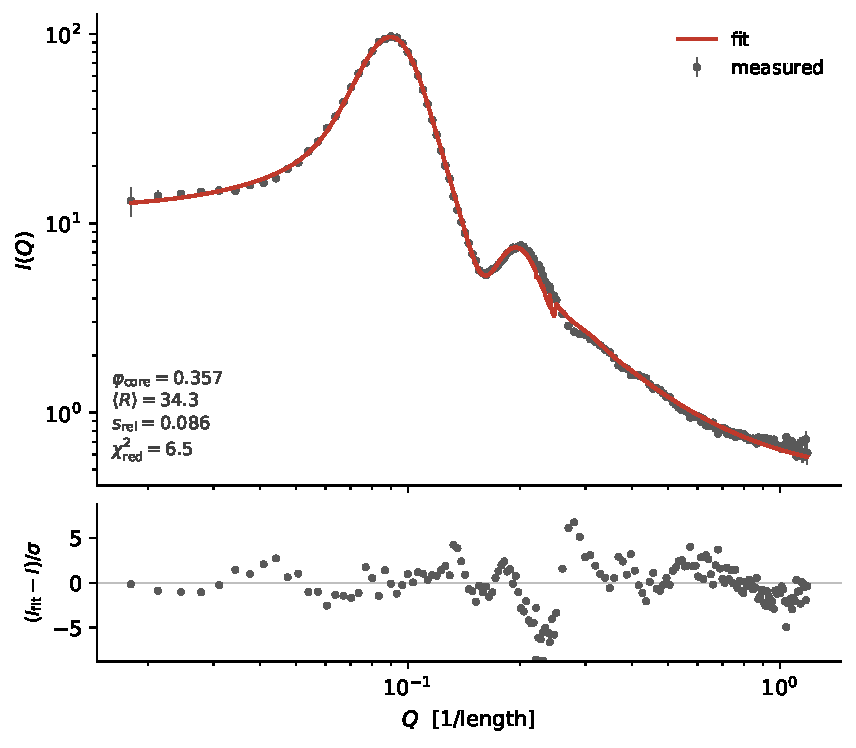
\includegraphics[width=\textwidth]{fig_realdata_fit.pdf}
\caption{The measured curve and the fit of Section~\ref{sec:realfit}. Upper
panel: data with error bars and the fitted model, over two decades in $Q$.
Lower panel: residuals in units of the error bar,
$(I_{\mathrm{fit}}-I)/\sigma$, which is the scale on which the reduced
$\chi^2$ of 6.5 is actually incurred --- on a log-intensity plot the
structure responsible is invisible.
The residuals are not random: they scatter within about $\pm 2\sigma$ at low
and high $Q$ but excur to $-7\sigma$ near $Q \approx 0.22$ to $0.28$, and
change character either side of $Q \approx 0.2$. That is the overlap region
between the two instrument geometries from which this curve was merged by
eye, and also where the form-factor minimum makes the model most sensitive.
The $\chi^2$ is therefore dominated by a localised defect in the data rather
than by the model missing it everywhere, which is what makes the volume
fraction --- fixed by the low-$Q$ level and the peak position --- trustworthy
despite it.
Drawn by \code{tools/fig\_realdata\_fit.py} directly from the saved session,
so the figure and the numbers quoted in the text cannot drift apart.}
\label{fig:realdatafit}
\end{figure}

The distinction is worth labouring, because getting it wrong is both easy
and self-confirming. Reading the solver's $\varphi$ as the particle volume
fraction reports a $10\,\%$ discrepancy --- and the grid-alignment bias of
Section~\ref{sec:verification} has the right sign and roughly the right
magnitude to explain it. That explanation would have been plausible,
tidy and wrong.

\paragraph{Two caveats belong with the number.} The reduced $\chi^2$ is
$6.5$, which is a statement about the data rather than the model: the curve
is merged from two instrument geometries of different resolution, aligned by
eye rather than numerically, and a scale mismatch between the sections is
penalised quadratically where the error bars are smallest. Fitting a
separate scale per section would reduce it and is not implemented. Second, a
ten-start search found six distinct minima, so the agreement holds at the
minimum reported rather than at a unique solution.

The volume fraction is nonetheless the robust quantity here. It is fixed by
the low-$Q$ level and the position of the structure-factor peak, not by the
relative scaling of the two sections, so the defect in the data misses what
is being checked. The parameters that the merge WOULD affect are those
constrained by the overlap region --- the width and the shell --- and should
be read accordingly.

Finally, this fit postdates the defects of Section~\ref{sec:verification}
and of the supplement, each of which affected every fit made before it was
corrected. That ordering is what makes the agreement meaningful rather than
fortunate.

% ---------------------------------------------------------------------
\section{Practical recommendations}

\begin{itemize}\itemsep2pt
\item Three moment-matched size classes suffice for the structure factor, but
the form-factor average needs of order forty; use
$p_F \gtrsim \Q_{\max}\langle\sigma\rangle s$.
\item Resolve the narrowest feature of the potential, not the particle. For a
well of width $\delta$, use $\gtrsim 30\,\sigma/\delta$ points per diameter;
the default of 100 makes a $\delta = 0.02\sigma$ well two grid points wide and
$S(\Q)$ ninety per cent wrong, without warning.
\item A small residual does not mean a correct solve. The closure equations
admit multiple fixed points; screen for $\min S(\Q) \ge 0$.
\item Solver convergence flags cannot be trusted; recompute the residual.
\item Include instrumental resolution when fitting measured data. Omitting it
biases the fitted polydispersity upward while leaving $\chi^2$ acceptable.
\item Report the parameter correlation matrix, not only error bars. In a
representative hard-sphere fit the radius and volume fraction correlate at
$0.75$, so quoting them as independent overstates what the data determines.
\item Near the critical point no closure of this family converges. The
self-consistent Ornstein--Zernike approximation (H\o ye \& Stell) is the
appropriate theory there, at the cost of solving a partial differential
equation over the whole density--temperature plane.
\end{itemize}

% ---------------------------------------------------------------------
\section{Conclusions}

The exact treatment of polydispersity in structure-factor modelling is no
longer expensive enough to justify approximating it by default. Combining
moment-matched discretisation with accelerated multicomponent OZ solvers gives
exact partial structure factors in a fraction of a second, for arbitrary pair
potentials and twenty-four closure relations, and allows the commonly used
decoupling approximations to be assessed against the exact result for the
specific system under study rather than assumed to hold.

% ---------------------------------------------------------------------
\section*{Open items before submission}
\begin{enumerate}\itemsep1pt
\item \S\ref{sec:schemes}: the systematic survey is DONE --- 120 converged
state points across four systems, replacing the four- and nine-point trials
whose conclusions it overturned. Note that section has been rewritten five
times, on 4, 9, 60, 98 and 120 points, and each version supported a different
conclusion; do not tighten its language without adding state points first.
The adhesive row is complete and a second Yukawa parameter set has been
added, so the regime picture no longer rests on a single slice.
\item \textbf{A fit to real measured data: done, and it validates the
volume fraction against an independent measurement.} The dataset is a merged
small-angle scattering curve from a colloidal sample whose volume fraction is
known by other means to be $0.392 \pm 0.005$. Fitted with a log-normal size
distribution, the Verlet closure, a core--shell form factor and resolution
smearing taken from the measured $\mathrm{d}Q$ column, the model returns a
hard-core volume fraction of $0.357$. Counting the shell into the particle
volume --- its thickness is linked to the distribution width here,
$\delta = c\,\mathrm{d}R$ --- and averaging $(R+\delta)^3$ over the fitted
distribution gives $\varphi = 0.388$, agreeing with the measured value to
within $0.8\sigma$.

This is a stronger check than the analytic comparisons elsewhere, and
different in kind. Those test the numerics against another calculation; this
tests the whole chain --- closure, discretisation, polydispersity, resolution
and form factor together --- against a quantity measured by means that know
nothing about any of it.

Two caveats belong with the number. The reduced $\chi^2$ is $6.5$, and that
is a statement about the data rather than the model: the curve is merged from
two instrument geometries of different resolution, aligned by eye rather than
numerically, and a scale mismatch between the sections is penalised
quadratically exactly where the error bars are smallest. Fitting a separate
scale per section would reduce it, and is future work. Second, a ten-start
search found six distinct minima, so the agreement holds at the minimum
reported rather than at a unique solution. The volume fraction is
nonetheless the robust quantity here: it is fixed by the low-$Q$ level and
the peak position rather than by the relative scaling of the two sections,
which is why it survives a merge that visibly costs $\chi^2$.

That this fit POSTDATES the defects listed below matters, since each
affected every fit made before it was corrected: the rank-revealing
linear solve returning zeros at a condition number of $10^{20}$, a fit-flag
reset that silently left only one parameter free, and a Gaussian resolution
kernel used where $\mathrm{d}Q/Q$ reached $0.55$.

\item \textbf{The transform type needs a decision, not just a
description.} Measured against the exact Percus--Yevick compressibility, the
first-order DST-I gives $S(0)$ low by $5.27\,\%$ at $\varphi = 0.40$ against
$0.036\,\%$ for the second-order DST-IV on the same grid --- a factor of 148,
because the hard core falls ON a type-1 node and BETWEEN type-4 nodes. Since
$S(0)$ is the compressibility, this is a systematic bias in exactly the
quantity $\varphi$ controls, and a fit absorbs it by moving $\varphi$.

Type 4 is nonetheless NOT the default, and cannot be for the polydisperse
route at all: it requires every pair core between grid points and the
$\sigma_{ij}$ of a moment-matched quadrature are mutually incommensurate.
Decide whether to default the one-component path to type 4, and state the
polydisperse limitation where a reader will meet it rather than only in the
validation section.

\item \textbf{The RMSA row is now qualified and the claim should be read
again.} ``Exact (9/9)'' held at nine state points where the Hayter--Penfold
rescaling never engaged. Where it does, the rescaled volume fraction still
agrees with the reference to four decimals but the curves agree only to
between $10^{-14}$ and $3\times10^{-5}$, degrading with coupling strength,
and one of nine fails to converge outright. Decide how much of that belongs
in the table and how much in the text.

\item \textbf{The report and this manuscript keep separate bibliographies
for the same papers} --- \code{daguanno1991} against
\code{DAguannoKlein1991}, 36 entries in all. A correction to one does not
reach the other, which is how the Carbajal--Tinoco closure carried a wrong
attribution in two documents at once. All 36 already have counterparts in
\code{ozgui.bib}; unifying them is a rename plus a switch from
\code{thebibliography}, to be done in one pass and matched on TITLES rather
than author surnames, since a surname match is what conflated two papers by
the same author in the first place.
\item The introduction's literature framing: PARTLY DONE. It now places the
work against the analytic solutions, the general-purpose solvers and the
scattering packages, and states the gap the software fills. That framing
rests on the packages actually used during development and validation, which
is not a systematic survey; check in particular whether any package now
combines exact multicomponent solution with arbitrary closures, and expand
the prior polydisperse OZ work beyond \citet{DAguannoKlein1991}.
\item Timings: DONE. Measured with \code{tools/benchmark.py} on a stated
machine and tabulated in \S\ref{sec:timing}. Re-run that script if the
hardware or the solver set changes; it writes JSON incrementally, so a
failure in one block does not discard the others.
\item Author list, acknowledgements, funding, data availability.
\item AI-assistance disclosure: a statement has been DRAFTED (see \S``Use of
AI assistance'' at the end of this document). It still needs checking against
IUCr's own policy, which may prescribe wording or placement, and the author
should confirm that the description of the division of labour matches their
own view of it.
included.
\item Transfer to the IUCr document class.
\end{enumerate}

% ---------------------------------------------------------------------
\begin{figure}[htbp]
\centering
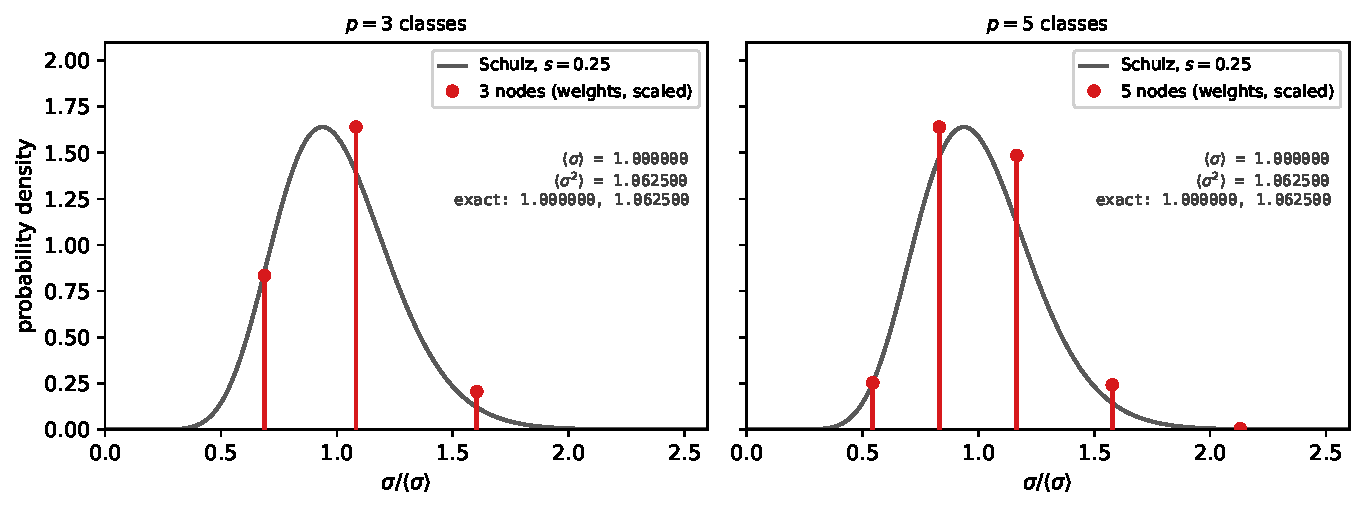
\includegraphics[width=\textwidth]{fig1_discretisation.pdf}
\caption{Moment-matched discretisation of a Schulz distribution of relative
width $s=0.25$ (solid line) into three (left) and five (right) size classes,
shown as the nodes and weights of the generalised Gauss--Laguerre rule. A
$p$-point rule reproduces the first $2p-1$ moments exactly.}
\label{fig:discretisation}
\end{figure}

\begin{figure}[htbp]
\centering
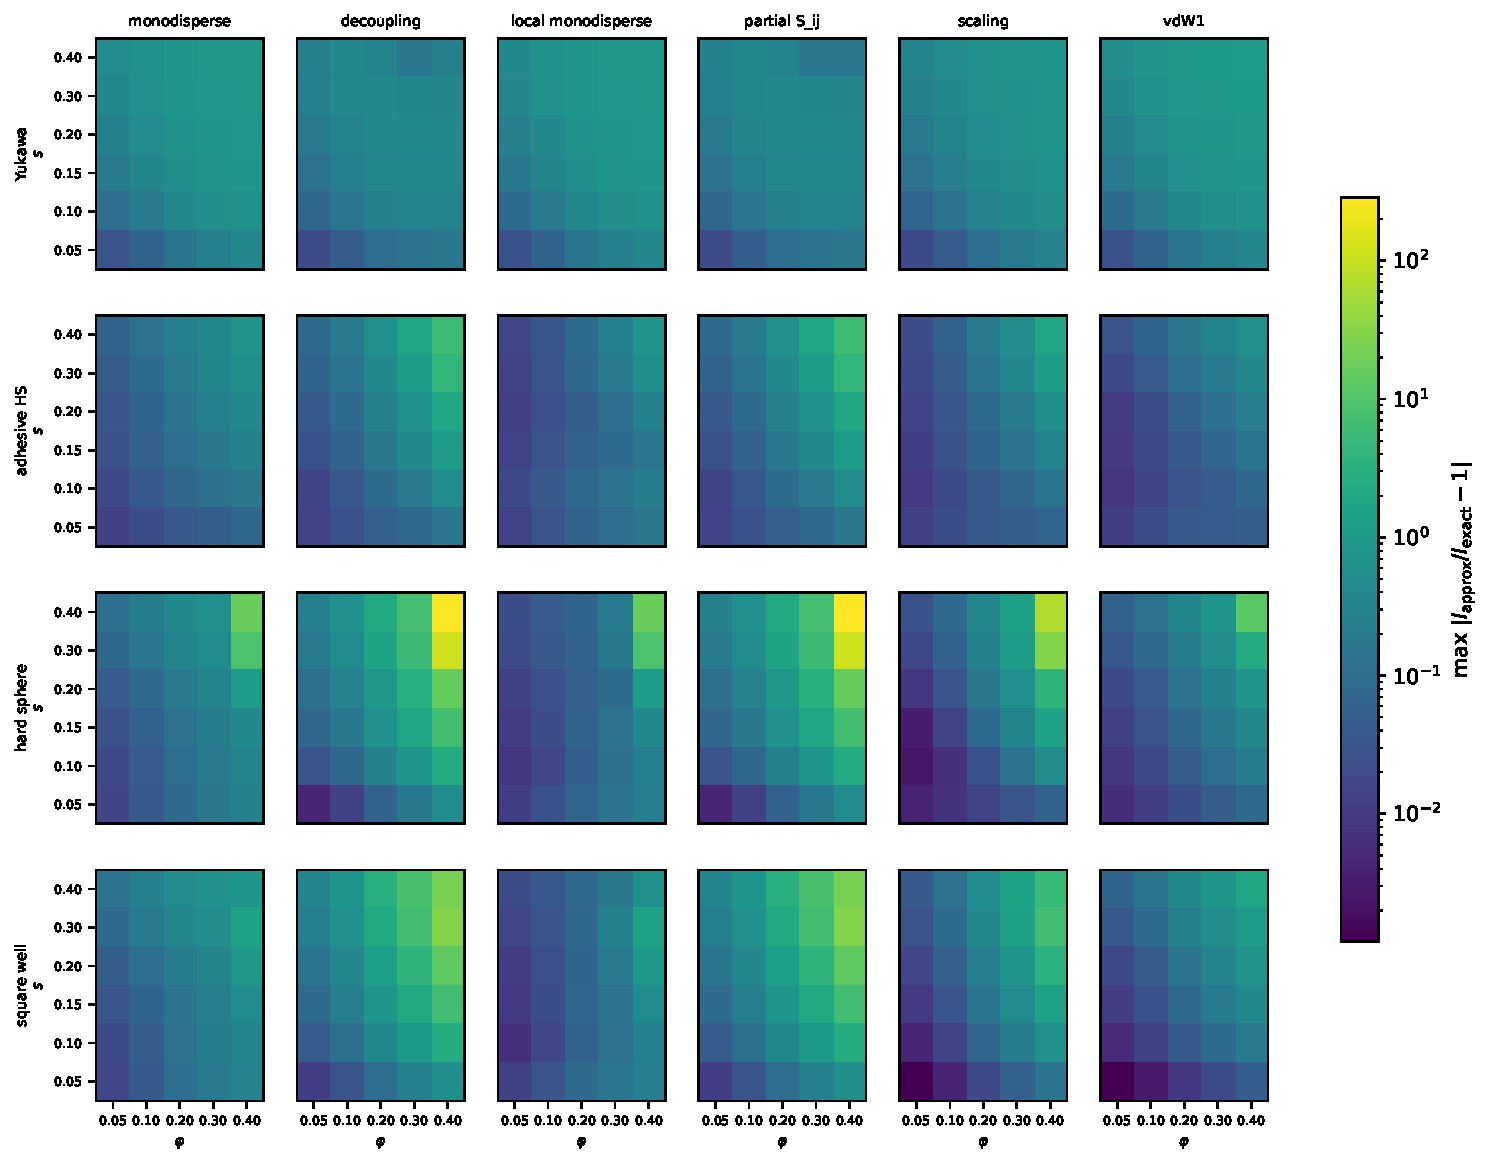
\includegraphics[width=\textwidth]{fig_survey.pdf}
\caption{Maximum relative error of each approximation scheme against the exact
multicomponent result, over the $(s,\varphi)$ plane, for hard spheres (top)
and a square-well fluid (bottom). Sixty state points, all converged. The
colour scale is common to all panels and logarithmic, so the panels are
directly comparable. The decoupling and partial-structure-factor schemes
(second and fourth columns) fail together and most severely at high
polydispersity and high volume fraction, reaching a factor of 286 for hard
spheres at $s = \varphi = 0.40$; the local monodisperse and van der Waals
one-fluid schemes remain usable across most of the plane. Generated by
\code{tools/section53\_survey.py}.}
\label{fig:survey}
\end{figure}

%REMOVED: fig2_scheme_error.pdf.
%
%It showed the relative error of the six approximation schemes for four
%representative systems, and it predated the corrections of
%\S\ref{sec:validation} -- it was computed before the identical-cores defect
%was found and before the narrow-well resolution trap, so at least two of its
%four systems were wrong. Its own caption said so, which is not a state a
%figure should stay in.
%
%fig_survey.pdf supersedes it completely: same comparison, 120 converged
%state points instead of four, on corrected code, with a common logarithmic
%colour scale so the panels are directly comparable. Keeping both would mean
%printing a known-wrong figure next to the one that replaced it.
%
%The file is still in figures/ if the old version is ever wanted for
%comparison. To bring a corrected version back, regenerate from the survey:
%    python tools/section53_survey.py --plot survey.jsonl

\begin{figure}[htbp]
\centering
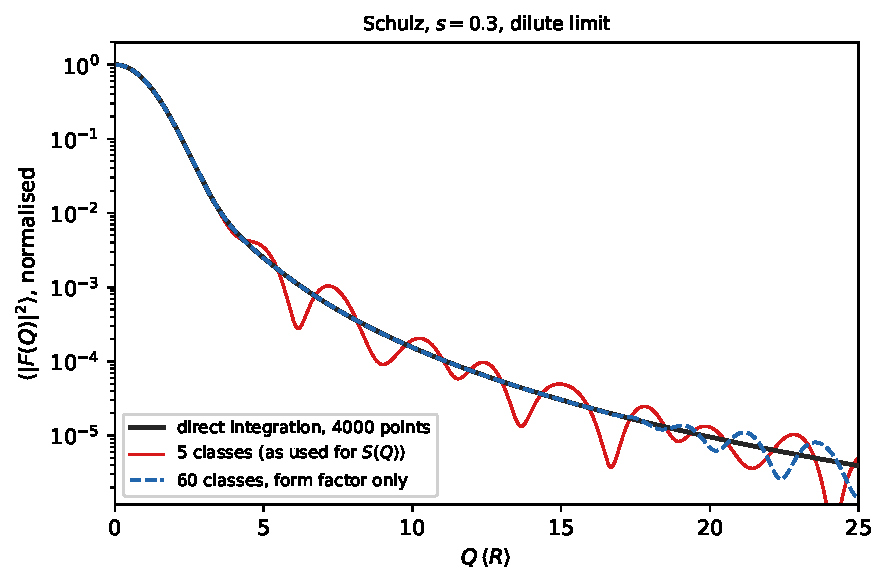
\includegraphics[width=0.6\textwidth]{fig3_oscillation.pdf}
\caption{Spurious form-factor oscillations from an inadequate discretisation of
the form-factor average, for a Schulz distribution of width $s=0.3$ in the
dilute limit. Direct integration with 4000 points (black) is essentially
smooth; evaluating on the same five classes used for the structure factor (red)
superposes five ringing form factors. Sixty classes for the form-factor average
alone (blue, dashed) restores the correct envelope.}
\label{fig:oscillation}
\end{figure}

\begin{figure}[htbp]
\centering
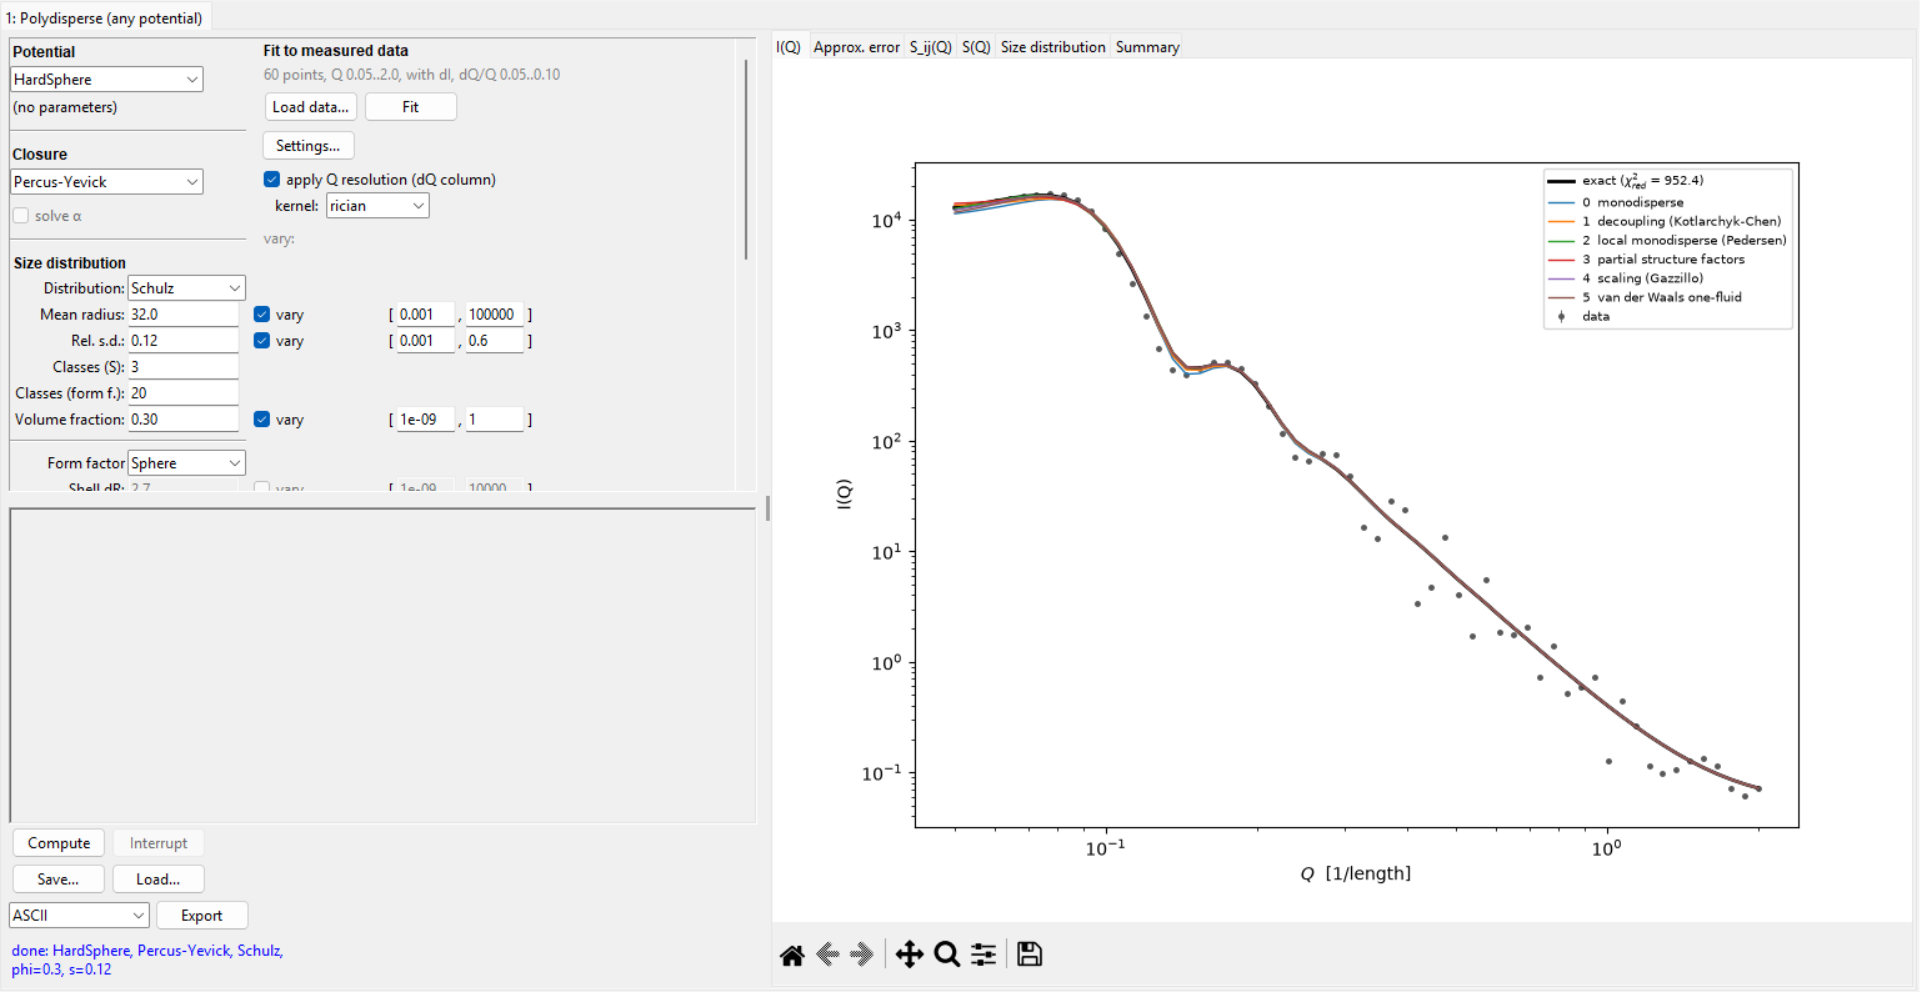
\includegraphics[width=0.85\textwidth]{gui_controls.png}
\caption{The polydisperse interface. Potential and closure parameter fields are
generated by introspection of the corresponding setter; the size-distribution
block carries separate class counts for the structure factor and the
form-factor average (\S\ref{sec:nff}).}
\label{fig:controls}
\end{figure}

\begin{figure}[htbp]
\centering
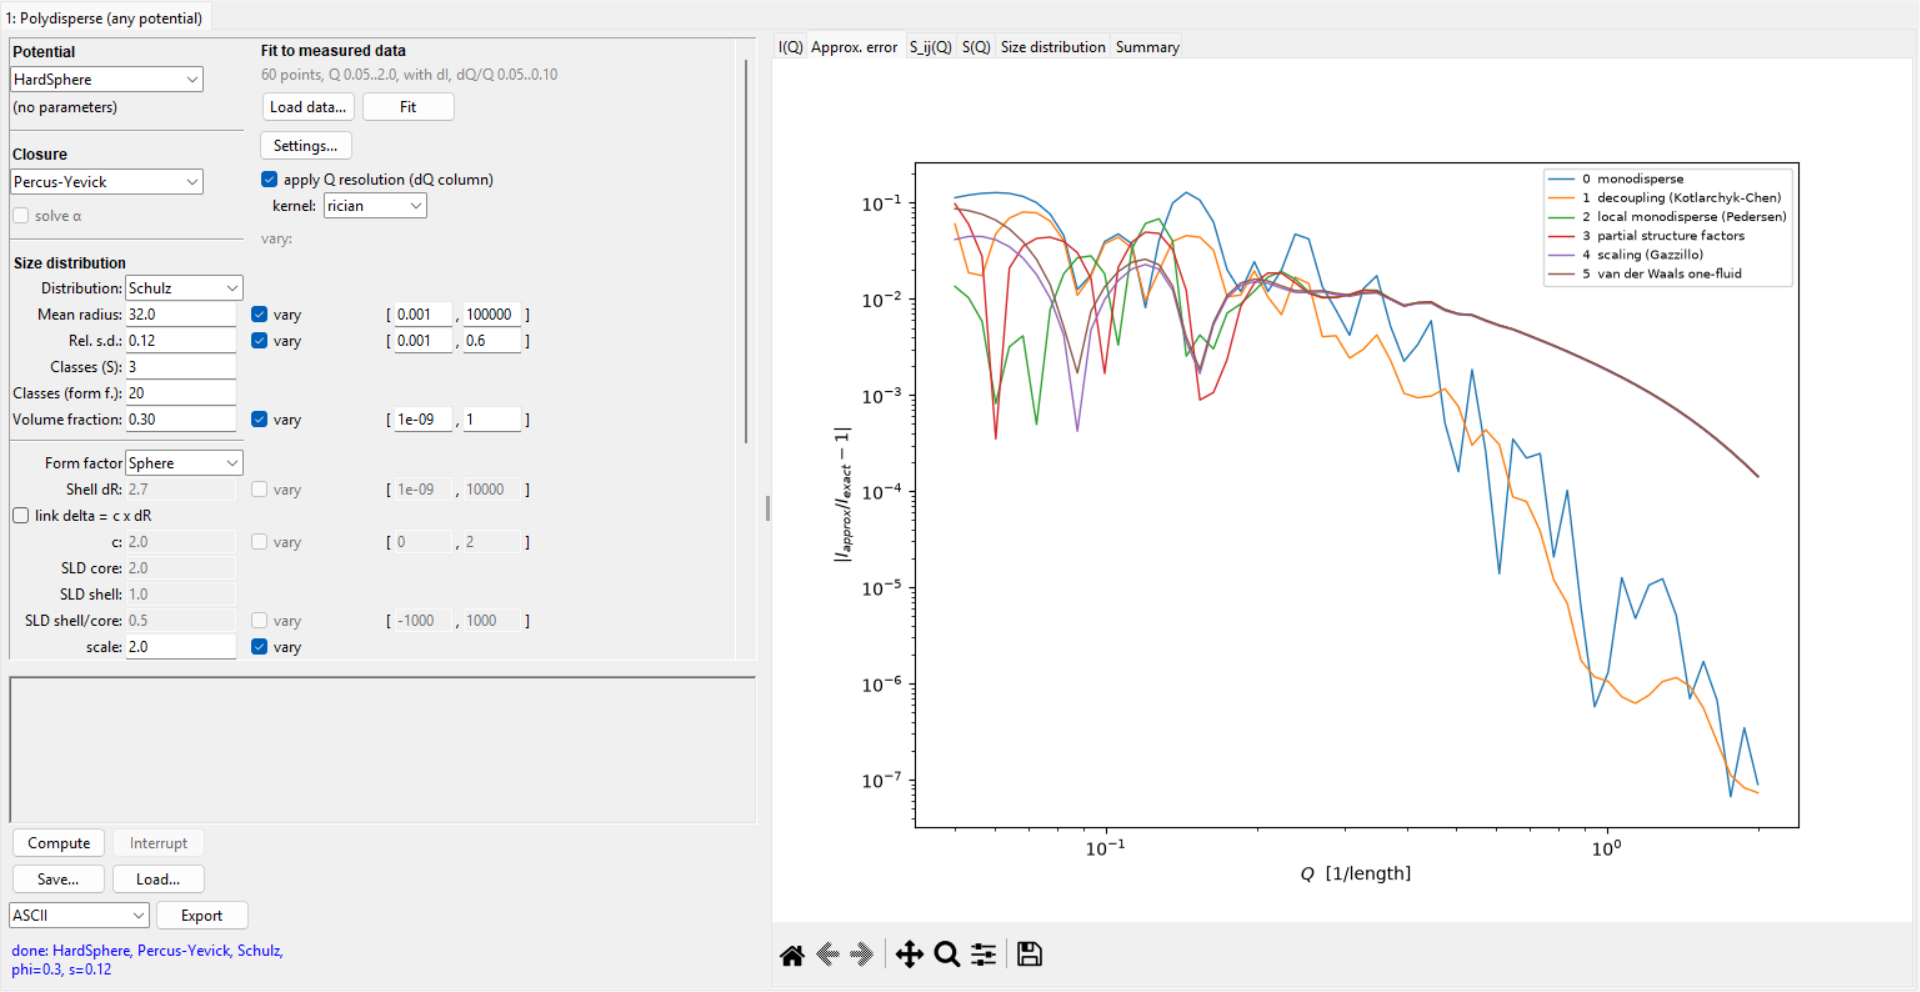
\includegraphics[width=0.85\textwidth]{gui_error.png}
\caption{The approximation-error panel, showing the relative error of all six
schemes against the exact result for the system currently under study. This is
the comparison the software is intended to make routine.}
\label{fig:guierror}
\end{figure}

% ---------------------------------------------------------------------
\section*{Software availability}

The software is distributed with SASfit. [COMPLETE BEFORE SUBMISSION:
repository URL, version tag or DOI, licence.]

\section*{Use of AI assistance}

Parts of the implementation, its test suite and this manuscript were
developed with the assistance of a large language model, used
interactively as a programming and drafting aid throughout. Its
contribution was concentrated in writing and refactoring code, constructing
validation scripts against external reference implementations, and drafting
and revising text. All physical content, the choice of models and closures,
the design of the validation strategy, and every numerical result reported
here were checked by the author; several of the errors described in
\S\ref{sec:validation} were found precisely because results produced with
such assistance were not taken on trust.

We note this not only because disclosure is expected but because it is
methodologically relevant. Software written this way accumulates plausible
but unverified assertions particularly easily --- a convergence flag read as
evidence of a solution, an approximation assumed cheap because it looked
cheap, an identical-cores defect that produced entirely reasonable-looking
structure factors. The emphasis throughout this paper on validating against
independent implementations, and on checking residuals rather than trusting
solver reports, is a direct response to that.

% ---------------------------------------------------------------------
%The bibliography is ../ozgui.bib, shared with the report. Do not add
%entries here -- add them there. build.sh runs bibtex between the pdflatex
%passes; without that pass every citation renders as (?).
%
%\nocite{*} WAS here, to stop the reference list silently shrinking to the
%handful of entries cited when the hand-written list was replaced. It has
%been REMOVED, because ozgui.bib is now shared with the report and holds 67
%entries: \nocite{*} would print all of them, including thirty-five closure
%papers this manuscript never cites. Only cited entries now appear, which is
%the correct behaviour.
%
%Consequence to watch: the printed list is now exactly what the text cites,
%currently about thirteen entries. If a reference that ought to be there has
%vanished, the fix is to CITE it in the text, not to restore \nocite{*}.
%unsrtnat numbers entries in order of first citation, which is the usual
%convention for a numbered list. Use plainnat instead for alphabetical order
%with numbers; both are natbib-compatible.
\bibliographystyle{unsrtnat}
\bibliography{../ozgui}

\end{document}
